\documentclass[twoside]{book}

% Packages required by doxygen
\usepackage{fixltx2e}
\usepackage{calc}
\usepackage{doxygen}
\usepackage[export]{adjustbox} % also loads graphicx
\usepackage{graphicx}
\usepackage[utf8]{inputenc}
\usepackage{makeidx}
\usepackage{multicol}
\usepackage{multirow}
\PassOptionsToPackage{warn}{textcomp}
\usepackage{textcomp}
\usepackage[nointegrals]{wasysym}
\usepackage[table]{xcolor}

% Font selection
\usepackage[T1]{fontenc}
\usepackage[scaled=.90]{helvet}
\usepackage{courier}
\usepackage{amssymb}
\usepackage{sectsty}
\renewcommand{\familydefault}{\sfdefault}
\allsectionsfont{%
  \fontseries{bc}\selectfont%
  \color{darkgray}%
}
\renewcommand{\DoxyLabelFont}{%
  \fontseries{bc}\selectfont%
  \color{darkgray}%
}
\newcommand{\+}{\discretionary{\mbox{\scriptsize$\hookleftarrow$}}{}{}}

% Page & text layout
\usepackage{geometry}
\geometry{%
  a4paper,%
  top=2.5cm,%
  bottom=2.5cm,%
  left=2.5cm,%
  right=2.5cm%
}
\tolerance=750
\hfuzz=15pt
\hbadness=750
\setlength{\emergencystretch}{15pt}
\setlength{\parindent}{0cm}
\setlength{\parskip}{3ex plus 2ex minus 2ex}
\makeatletter
\renewcommand{\paragraph}{%
  \@startsection{paragraph}{4}{0ex}{-1.0ex}{1.0ex}{%
    \normalfont\normalsize\bfseries\SS@parafont%
  }%
}
\renewcommand{\subparagraph}{%
  \@startsection{subparagraph}{5}{0ex}{-1.0ex}{1.0ex}{%
    \normalfont\normalsize\bfseries\SS@subparafont%
  }%
}
\makeatother

% Headers & footers
\usepackage{fancyhdr}
\pagestyle{fancyplain}
\fancyhead[LE]{\fancyplain{}{\bfseries\thepage}}
\fancyhead[CE]{\fancyplain{}{}}
\fancyhead[RE]{\fancyplain{}{\bfseries\leftmark}}
\fancyhead[LO]{\fancyplain{}{\bfseries\rightmark}}
\fancyhead[CO]{\fancyplain{}{}}
\fancyhead[RO]{\fancyplain{}{\bfseries\thepage}}
\fancyfoot[LE]{\fancyplain{}{}}
\fancyfoot[CE]{\fancyplain{}{}}
\fancyfoot[RE]{\fancyplain{}{\bfseries\scriptsize Generated by Doxygen }}
\fancyfoot[LO]{\fancyplain{}{\bfseries\scriptsize Generated by Doxygen }}
\fancyfoot[CO]{\fancyplain{}{}}
\fancyfoot[RO]{\fancyplain{}{}}
\renewcommand{\footrulewidth}{0.4pt}
\renewcommand{\chaptermark}[1]{%
  \markboth{#1}{}%
}
\renewcommand{\sectionmark}[1]{%
  \markright{\thesection\ #1}%
}

% Indices & bibliography
\usepackage{natbib}
\usepackage[titles]{tocloft}
\setcounter{tocdepth}{3}
\setcounter{secnumdepth}{5}
\makeindex

% Hyperlinks (required, but should be loaded last)
\usepackage{ifpdf}
\ifpdf
  \usepackage[pdftex,pagebackref=true]{hyperref}
\else
  \usepackage[ps2pdf,pagebackref=true]{hyperref}
\fi
\hypersetup{%
  colorlinks=true,%
  linkcolor=blue,%
  citecolor=blue,%
  unicode%
}

% Custom commands
\newcommand{\clearemptydoublepage}{%
  \newpage{\pagestyle{empty}\cleardoublepage}%
}

\usepackage{caption}
\captionsetup{labelsep=space,justification=centering,font={bf},singlelinecheck=off,skip=4pt,position=top}

%===== C O N T E N T S =====

\begin{document}

% Titlepage & ToC
\hypersetup{pageanchor=false,
             bookmarksnumbered=true,
             pdfencoding=unicode
            }
\pagenumbering{roman}
\begin{titlepage}
\vspace*{7cm}
\begin{center}%
{\Large I\+F2210\+\_\+\+Tubes1\+\_\+\+Animal\textquotesingle{}s Village \\[1ex]\large v3 }\\
\vspace*{1cm}
{\large Generated by Doxygen 1.8.11}\\
\end{center}
\end{titlepage}
\clearemptydoublepage
\tableofcontents
\clearemptydoublepage
\pagenumbering{arabic}
\hypersetup{pageanchor=true}

%--- Begin generated contents ---
\chapter{Hierarchical Index}
\section{Class Hierarchy}
This inheritance list is sorted roughly, but not completely, alphabetically\+:\begin{DoxyCompactList}
\item \contentsline{section}{Exception\+Object}{\pageref{class_exception_object}}{}
\item \contentsline{section}{I\+O\+Manager}{\pageref{class_i_o_manager}}{}
\begin{DoxyCompactList}
\item \contentsline{section}{Screen}{\pageref{class_screen}}{}
\item \contentsline{section}{Snapshot\+Capturer}{\pageref{class_snapshot_capturer}}{}
\end{DoxyCompactList}
\item \contentsline{section}{Keypress\+Handler}{\pageref{class_keypress_handler}}{}
\item \contentsline{section}{L\+Makhluk}{\pageref{class_l_makhluk}}{}
\item \contentsline{section}{Makhluk}{\pageref{class_makhluk}}{}
\begin{DoxyCompactList}
\item \contentsline{section}{Hewan}{\pageref{class_hewan}}{}
\begin{DoxyCompactList}
\item \contentsline{section}{Polar\+Bear}{\pageref{class_polar_bear}}{}
\item \contentsline{section}{Rabbit}{\pageref{class_rabbit}}{}
\item \contentsline{section}{Sheep}{\pageref{class_sheep}}{}
\item \contentsline{section}{Snake}{\pageref{class_snake}}{}
\item \contentsline{section}{Turtle}{\pageref{class_turtle}}{}
\item \contentsline{section}{Wolf}{\pageref{class_wolf}}{}
\end{DoxyCompactList}
\item \contentsline{section}{Tumbuhan}{\pageref{class_tumbuhan}}{}
\end{DoxyCompactList}
\item \contentsline{section}{Matrix}{\pageref{class_matrix}}{}
\item \contentsline{section}{Point}{\pageref{class_point}}{}
\item \contentsline{section}{Random\+Generator}{\pageref{class_random_generator}}{}
\item \contentsline{section}{World}{\pageref{class_world}}{}
\item \contentsline{section}{World\+Builder}{\pageref{class_world_builder}}{}
\end{DoxyCompactList}

\chapter{Class Index}
\section{Class List}
Here are the classes, structs, unions and interfaces with brief descriptions\+:\begin{DoxyCompactList}
\item\contentsline{section}{\hyperlink{class_exception_object}{Exception\+Object} \\*Kelas untuk membantu menangani exception yang muncul dari kesalahan masukan pengguna }{\pageref{class_exception_object}}{}
\item\contentsline{section}{\hyperlink{class_hewan}{Hewan} \\*Abstract Base Class yang merupakan Kelas Turunan dari \hyperlink{class_makhluk}{Makhluk} }{\pageref{class_hewan}}{}
\item\contentsline{section}{\hyperlink{class_i_o_manager}{I\+O\+Manager} \\*Abstract Base Class yang merupakan kelas dasar Input/\+Output }{\pageref{class_i_o_manager}}{}
\item\contentsline{section}{\hyperlink{class_keypress_handler}{Keypress\+Handler} \\*Handler untuk masukan dari user berupa keypress }{\pageref{class_keypress_handler}}{}
\item\contentsline{section}{\hyperlink{class_l_makhluk}{L\+Makhluk} \\*Representasi A\+DT List of \hyperlink{class_makhluk}{Makhluk} }{\pageref{class_l_makhluk}}{}
\item\contentsline{section}{\hyperlink{class_makhluk}{Makhluk} \\*Representasi dari makhluk di alam semesta }{\pageref{class_makhluk}}{}
\item\contentsline{section}{\hyperlink{class_matrix}{Matrix} \\*Representasi array dua dimensi }{\pageref{class_matrix}}{}
\item\contentsline{section}{\hyperlink{class_point}{Point} \\*Representasi titik dalam koordinat kartesian }{\pageref{class_point}}{}
\item\contentsline{section}{\hyperlink{class_polar_bear}{Polar\+Bear} \\*Kelas turunan dari \hyperlink{class_makhluk}{Makhluk} berupa \hyperlink{class_polar_bear}{Polar\+Bear} }{\pageref{class_polar_bear}}{}
\item\contentsline{section}{\hyperlink{class_rabbit}{Rabbit} \\*Kelas Turunan dari \hyperlink{class_makhluk}{Makhluk} berupa \hyperlink{class_rabbit}{Rabbit} }{\pageref{class_rabbit}}{}
\item\contentsline{section}{\hyperlink{class_random_generator}{Random\+Generator} \\*Mengembalikan random number }{\pageref{class_random_generator}}{}
\item\contentsline{section}{\hyperlink{class_screen}{Screen} \\*Representasi dari layar pengguna }{\pageref{class_screen}}{}
\item\contentsline{section}{\hyperlink{class_sheep}{Sheep} \\*Kelas turunan dari \hyperlink{class_makhluk}{Makhluk} berupa \hyperlink{class_sheep}{Sheep} }{\pageref{class_sheep}}{}
\item\contentsline{section}{\hyperlink{class_snake}{Snake} \\*Kelas Turunan dari \hyperlink{class_makhluk}{Makhluk} berupa \hyperlink{class_snake}{Snake} }{\pageref{class_snake}}{}
\item\contentsline{section}{\hyperlink{class_snapshot_capturer}{Snapshot\+Capturer} \\*Kelas untuk mengambil snapshot state dunia }{\pageref{class_snapshot_capturer}}{}
\item\contentsline{section}{\hyperlink{class_tumbuhan}{Tumbuhan} \\*Kelas Turunan dari \hyperlink{class_makhluk}{Makhluk} berupa \hyperlink{class_tumbuhan}{Tumbuhan} }{\pageref{class_tumbuhan}}{}
\item\contentsline{section}{\hyperlink{class_turtle}{Turtle} \\*Kelas Turunan dari \hyperlink{class_makhluk}{Makhluk} berupa \hyperlink{class_turtle}{Turtle} }{\pageref{class_turtle}}{}
\item\contentsline{section}{\hyperlink{class_wolf}{Wolf} \\*Kelas turunan dari \hyperlink{class_makhluk}{Makhluk} berupa \hyperlink{class_wolf}{Wolf} }{\pageref{class_wolf}}{}
\item\contentsline{section}{\hyperlink{class_world}{World} \\*Representasi dari alam semesta }{\pageref{class_world}}{}
\item\contentsline{section}{\hyperlink{class_world_builder}{World\+Builder} \\*Builder kelas \hyperlink{class_world}{World} }{\pageref{class_world_builder}}{}
\end{DoxyCompactList}

\chapter{Class Documentation}
\hypertarget{class_exception_object}{}\section{Exception\+Object Class Reference}
\label{class_exception_object}\index{Exception\+Object@{Exception\+Object}}


Kelas untuk membantu menangani exception yang muncul dari kesalahan masukan pengguna.  




{\ttfamily \#include $<$Exception\+Object.\+h$>$}

\subsection*{Public Member Functions}
\begin{DoxyCompactItemize}
\item 
\hyperlink{class_exception_object_a25372a2efb503791bd5be72d320b6025}{Exception\+Object} (int)
\begin{DoxyCompactList}\small\item\em Constructor. \end{DoxyCompactList}\item 
void \hyperlink{class_exception_object_a79bec5cf1474c4fab59b09e2829bf4f2}{Display\+Error\+Message} ()
\begin{DoxyCompactList}\small\item\em Prosedur untuk menampilkan pesan kesalahan. \end{DoxyCompactList}\end{DoxyCompactItemize}


\subsection{Detailed Description}
Kelas untuk membantu menangani exception yang muncul dari kesalahan masukan pengguna. 

Kelas \hyperlink{class_exception_object}{Exception\+Object} menyediakan sebuah instance untuk dilempar ke Exception\+Handler apabila masukan pengguna salah \begin{DoxyAuthor}{Author}
Robert Sebastian Herlim 
\end{DoxyAuthor}
\begin{DoxyDate}{Date}
Maret 2016 
\end{DoxyDate}


\subsection{Constructor \& Destructor Documentation}
\index{Exception\+Object@{Exception\+Object}!Exception\+Object@{Exception\+Object}}
\index{Exception\+Object@{Exception\+Object}!Exception\+Object@{Exception\+Object}}
\subsubsection[{\texorpdfstring{Exception\+Object(int)}{ExceptionObject(int)}}]{\setlength{\rightskip}{0pt plus 5cm}Exception\+Object\+::\+Exception\+Object (
\begin{DoxyParamCaption}
\item[{int}]{\+\_\+\+ID}
\end{DoxyParamCaption}
)}\hypertarget{class_exception_object_a25372a2efb503791bd5be72d320b6025}{}\label{class_exception_object_a25372a2efb503791bd5be72d320b6025}


Constructor. 

Menciptakan sebuah instance dari kelas \hyperlink{class_exception_object}{Exception\+Object} dengan id yang di-\/passing melalui parameter 
\begin{DoxyParams}{Parameters}
{\em \+\_\+\+ID} & int id yang merupakan id\+\_\+kesalahan yang dilakukan \\
\hline
\end{DoxyParams}


\subsection{Member Function Documentation}
\index{Exception\+Object@{Exception\+Object}!Display\+Error\+Message@{Display\+Error\+Message}}
\index{Display\+Error\+Message@{Display\+Error\+Message}!Exception\+Object@{Exception\+Object}}
\subsubsection[{\texorpdfstring{Display\+Error\+Message()}{DisplayErrorMessage()}}]{\setlength{\rightskip}{0pt plus 5cm}void Exception\+Object\+::\+Display\+Error\+Message (
\begin{DoxyParamCaption}
{}
\end{DoxyParamCaption}
)}\hypertarget{class_exception_object_a79bec5cf1474c4fab59b09e2829bf4f2}{}\label{class_exception_object_a79bec5cf1474c4fab59b09e2829bf4f2}


Prosedur untuk menampilkan pesan kesalahan. 

Menampilkan pesan kesalahan ke sebuah message box berdasarkan id\+\_\+kesalahan yang disimpan dalam data member 

The documentation for this class was generated from the following files\+:\begin{DoxyCompactItemize}
\item 
C\+:/\+Users/\+Ngiong/\+Documents/\+Git\+Hub/\+Tubes\+Makhluk/v3/header/Exception\+Object.\+h\item 
C\+:/\+Users/\+Ngiong/\+Documents/\+Git\+Hub/\+Tubes\+Makhluk/v3/implementation/Exception\+Object.\+cpp\end{DoxyCompactItemize}

\hypertarget{class_hewan}{}\section{Hewan Class Reference}
\label{class_hewan}\index{Hewan@{Hewan}}


Abstract Base Class yang merupakan Kelas Turunan dari \hyperlink{class_makhluk}{Makhluk}.  




{\ttfamily \#include $<$Hewan.\+h$>$}

Inheritance diagram for Hewan\+:\begin{figure}[H]
\begin{center}
\leavevmode
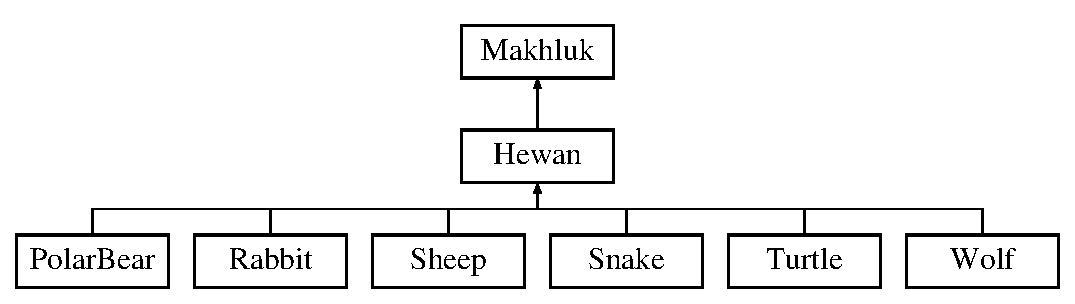
\includegraphics[height=3.000000cm]{class_hewan}
\end{center}
\end{figure}
\subsection*{Public Member Functions}
\begin{DoxyCompactItemize}
\item 
virtual void \hyperlink{class_hewan_aea0228b7a5fc5b15691affeff5ae3099}{Move} (int, int)
\begin{DoxyCompactList}\small\item\em Procedure virtual tidak pure untuk menggerakan objek bertipe turunan kelas \hyperlink{class_hewan}{Hewan}. \end{DoxyCompactList}\item 
virtual int \hyperlink{class_hewan_a90a316426af1d53add7ebf2a23ea9af2}{is\+Vegetarian} ()=0
\begin{DoxyCompactList}\small\item\em Fungsi pure virtual untuk validasi apakah sebuah objek adalah Vegetarian. \end{DoxyCompactList}\item 
virtual void \hyperlink{class_hewan_ab0478d48070dc3c51cda481f678ae40a}{Get\+To\+Food} ()=0
\begin{DoxyCompactList}\small\item\em Procedure virtual pure untuk objek mendapatkan makanannya. \end{DoxyCompactList}\item 
int \hyperlink{class_hewan_a09445ef7de5b3e43b5205ae0857581d5}{get\+Hunger\+Lvl} ()
\begin{DoxyCompactList}\small\item\em Fungsi getter untuk mendapatkan level kelaparan sebuah objek. \end{DoxyCompactList}\item 
int \hyperlink{class_hewan_ab7586f90668c11c1abaf64017f1e557d}{get\+Power} ()
\begin{DoxyCompactList}\small\item\em Fungsi getter untuk mendapatkan nilai power sebuah objek. \end{DoxyCompactList}\item 
int \hyperlink{class_hewan_a9b3d754b6faf3706aabe8dcaec6f1540}{get\+DeltaT} ()
\begin{DoxyCompactList}\small\item\em Fungsi getter untuk mendapatkan deltaT sebuah objek. \end{DoxyCompactList}\item 
void \hyperlink{class_hewan_a07b8d783d4712158dbcad234a1178e81}{set\+Hunger\+Lvl} (int x)
\begin{DoxyCompactList}\small\item\em Procedure setter untuk level kelaparan. \end{DoxyCompactList}\item 
void \hyperlink{class_hewan_a8268bfb533b9becb62e2bd8eee2e7960}{Wandering} ()
\begin{DoxyCompactList}\small\item\em Procedure berjalan random sebuah objek. \end{DoxyCompactList}\item 
void \hyperlink{class_hewan_ad1ba348d0912e3e392e41ae0c197c69b}{Sleep} ()
\begin{DoxyCompactList}\small\item\em Procedure tidur sebuah objek. \end{DoxyCompactList}\item 
\hyperlink{class_makhluk}{Makhluk} $\ast$ \hyperlink{class_hewan_ab604462c6b9c235f9d53d42235acd41b}{Find\+Food} ()
\begin{DoxyCompactList}\small\item\em Fungsi untuk objek menemukan makanannya. \end{DoxyCompactList}\item 
\hyperlink{class_makhluk}{Makhluk} $\ast$ \hyperlink{class_hewan_a7d89c8d0bee799698b986159c67f6bb3}{Find\+Makhluk} (char \+\_\+\+ID)
\begin{DoxyCompactList}\small\item\em Fungsi untuk objek mendapatkan sebuah \hyperlink{class_makhluk}{Makhluk}  Mendapatkan makhluk yang dicari berdasarkan ID pada list\+Makhluk. \end{DoxyCompactList}\item 
int \hyperlink{class_hewan_af4ae28e9179a2438a666b26e1882139d}{should\+Rebounced} (int dx, int dy)
\begin{DoxyCompactList}\small\item\em Fungsi validasi objek untuk Rebounce. \end{DoxyCompactList}\item 
bool \hyperlink{class_hewan_a3798162fd7aa8cfef947abce00c283ef}{is\+Makhlukin\+List} (char \+\_\+\+ID)
\begin{DoxyCompactList}\small\item\em Fungsi validasi apakah sebuah \hyperlink{class_makhluk}{Makhluk} ada di list\+Makhluk. \end{DoxyCompactList}\item 
void \hyperlink{class_hewan_a5420deb2ff65c6cedd5c80f1f3d42d00}{get\+To\+Point} (\hyperlink{class_point}{Point} P)
\begin{DoxyCompactList}\small\item\em Procedure agar objek berpindah ke suatu point. \end{DoxyCompactList}\item 
void \hyperlink{class_hewan_a375987dfe4052f14a6edd19c9b59937a}{move\+Toward\+Point} (\hyperlink{class_point}{Point} P)
\begin{DoxyCompactList}\small\item\em Procedure agar objek melangkah satu langkah mendekat ke suatu \hyperlink{class_point}{Point}. \end{DoxyCompactList}\end{DoxyCompactItemize}
\subsection*{Protected Member Functions}
\begin{DoxyCompactItemize}
\item 
\hyperlink{class_hewan_a5ea6a7a559331a71c86c59eaeb3809db}{Hewan} (char, int)
\begin{DoxyCompactList}\small\item\em Constructor. \end{DoxyCompactList}\end{DoxyCompactItemize}
\subsection*{Protected Attributes}
\begin{DoxyCompactItemize}
\item 
int \hyperlink{class_hewan_ac2181643305f48f23c648b58d5b662b5}{hunger\+Lvl}
\item 
int \hyperlink{class_hewan_a3fbf8081066fe2fb2b7b8cce149910a1}{power}
\item 
int \hyperlink{class_hewan_a7d22294907eb5b03983fdb179b248c18}{deltaT}
\end{DoxyCompactItemize}
\subsection*{Additional Inherited Members}


\subsection{Detailed Description}
Abstract Base Class yang merupakan Kelas Turunan dari \hyperlink{class_makhluk}{Makhluk}. 

Kelas \hyperlink{class_hewan}{Hewan} merupakan kelas yang berfungsi untuk mengimplementasikan behaviour yang yang dimiliki oleh turunan kelas \hyperlink{class_hewan}{Hewan} \begin{DoxyAuthor}{Author}
Atika Azzahra Akbar 
\end{DoxyAuthor}
\begin{DoxyDate}{Date}
Maret 2016 
\end{DoxyDate}


\subsection{Constructor \& Destructor Documentation}
\index{Hewan@{Hewan}!Hewan@{Hewan}}
\index{Hewan@{Hewan}!Hewan@{Hewan}}
\subsubsection[{\texorpdfstring{Hewan(char, int)}{Hewan(char, int)}}]{\setlength{\rightskip}{0pt plus 5cm}Hewan\+::\+Hewan (
\begin{DoxyParamCaption}
\item[{char}]{\+\_\+\+ID, }
\item[{int}]{\+\_\+max\+Age}
\end{DoxyParamCaption}
)\hspace{0.3cm}{\ttfamily [protected]}}\hypertarget{class_hewan_a5ea6a7a559331a71c86c59eaeb3809db}{}\label{class_hewan_a5ea6a7a559331a71c86c59eaeb3809db}


Constructor. 

Constructor \hyperlink{class_hewan}{Hewan} yang akan membentuk objek bertipe \hyperlink{class_hewan}{Hewan} yang dapat dicasting dengan objek bertipe turunan kelas \hyperlink{class_hewan}{Hewan} 
\begin{DoxyParams}{Parameters}
{\em character} & ID \hyperlink{class_makhluk}{Makhluk} \\
\hline
{\em integer} & max\+Age \hyperlink{class_makhluk}{Makhluk} \\
\hline
\end{DoxyParams}


\subsection{Member Function Documentation}
\index{Hewan@{Hewan}!Find\+Food@{Find\+Food}}
\index{Find\+Food@{Find\+Food}!Hewan@{Hewan}}
\subsubsection[{\texorpdfstring{Find\+Food()}{FindFood()}}]{\setlength{\rightskip}{0pt plus 5cm}{\bf Makhluk} $\ast$ Hewan\+::\+Find\+Food (
\begin{DoxyParamCaption}
{}
\end{DoxyParamCaption}
)}\hypertarget{class_hewan_ab604462c6b9c235f9d53d42235acd41b}{}\label{class_hewan_ab604462c6b9c235f9d53d42235acd41b}


Fungsi untuk objek menemukan makanannya. 

Mendapatkan makanan sebuah objek. Jika objek merupakan vegetarian akan dikembalikan objek bertipe tumbuhan dan jika bukan akan dikembalikan makhluk dengan power dibawah power objek tersebut \begin{DoxyReturn}{Returns}
pointer to \hyperlink{class_makhluk}{Makhluk} 
\end{DoxyReturn}
\index{Hewan@{Hewan}!Find\+Makhluk@{Find\+Makhluk}}
\index{Find\+Makhluk@{Find\+Makhluk}!Hewan@{Hewan}}
\subsubsection[{\texorpdfstring{Find\+Makhluk(char \+\_\+\+I\+D)}{FindMakhluk(char _ID)}}]{\setlength{\rightskip}{0pt plus 5cm}{\bf Makhluk} $\ast$ Hewan\+::\+Find\+Makhluk (
\begin{DoxyParamCaption}
\item[{char}]{\+\_\+\+ID}
\end{DoxyParamCaption}
)}\hypertarget{class_hewan_a7d89c8d0bee799698b986159c67f6bb3}{}\label{class_hewan_a7d89c8d0bee799698b986159c67f6bb3}


Fungsi untuk objek mendapatkan sebuah \hyperlink{class_makhluk}{Makhluk}  Mendapatkan makhluk yang dicari berdasarkan ID pada list\+Makhluk. 


\begin{DoxyParams}{Parameters}
{\em char} & ID dari \hyperlink{class_makhluk}{Makhluk} yang ingin dicari \\
\hline
\end{DoxyParams}
\begin{DoxyReturn}{Returns}
pointer to \hyperlink{class_makhluk}{Makhluk} 
\end{DoxyReturn}
\index{Hewan@{Hewan}!get\+DeltaT@{get\+DeltaT}}
\index{get\+DeltaT@{get\+DeltaT}!Hewan@{Hewan}}
\subsubsection[{\texorpdfstring{get\+Delta\+T()}{getDeltaT()}}]{\setlength{\rightskip}{0pt plus 5cm}int Hewan\+::get\+DeltaT (
\begin{DoxyParamCaption}
{}
\end{DoxyParamCaption}
)\hspace{0.3cm}{\ttfamily [inline]}}\hypertarget{class_hewan_a9b3d754b6faf3706aabe8dcaec6f1540}{}\label{class_hewan_a9b3d754b6faf3706aabe8dcaec6f1540}


Fungsi getter untuk mendapatkan deltaT sebuah objek. 

Mengembalikan deltaT sebuah objek bertipe turunan kelas \hyperlink{class_hewan}{Hewan} yang diinisialisasi saat ctor sebuah objek \begin{DoxyReturn}{Returns}
integer 
\end{DoxyReturn}
\index{Hewan@{Hewan}!get\+Hunger\+Lvl@{get\+Hunger\+Lvl}}
\index{get\+Hunger\+Lvl@{get\+Hunger\+Lvl}!Hewan@{Hewan}}
\subsubsection[{\texorpdfstring{get\+Hunger\+Lvl()}{getHungerLvl()}}]{\setlength{\rightskip}{0pt plus 5cm}int Hewan\+::get\+Hunger\+Lvl (
\begin{DoxyParamCaption}
{}
\end{DoxyParamCaption}
)\hspace{0.3cm}{\ttfamily [inline]}}\hypertarget{class_hewan_a09445ef7de5b3e43b5205ae0857581d5}{}\label{class_hewan_a09445ef7de5b3e43b5205ae0857581d5}


Fungsi getter untuk mendapatkan level kelaparan sebuah objek. 

Mengembalikan level kelaparan sebuah objek bertipe turunan kelas \hyperlink{class_hewan}{Hewan} yang diinisialisasi saat ctor sebuah objek \begin{DoxyReturn}{Returns}
integer 
\end{DoxyReturn}
\index{Hewan@{Hewan}!get\+Power@{get\+Power}}
\index{get\+Power@{get\+Power}!Hewan@{Hewan}}
\subsubsection[{\texorpdfstring{get\+Power()}{getPower()}}]{\setlength{\rightskip}{0pt plus 5cm}int Hewan\+::get\+Power (
\begin{DoxyParamCaption}
{}
\end{DoxyParamCaption}
)\hspace{0.3cm}{\ttfamily [inline]}}\hypertarget{class_hewan_ab7586f90668c11c1abaf64017f1e557d}{}\label{class_hewan_ab7586f90668c11c1abaf64017f1e557d}


Fungsi getter untuk mendapatkan nilai power sebuah objek. 

Mengembalikan nilai power sebuah objek bertipe turunan kelas \hyperlink{class_hewan}{Hewan} yang diinisialisasi saat ctor sebuah objek \begin{DoxyReturn}{Returns}
integer 
\end{DoxyReturn}
\index{Hewan@{Hewan}!Get\+To\+Food@{Get\+To\+Food}}
\index{Get\+To\+Food@{Get\+To\+Food}!Hewan@{Hewan}}
\subsubsection[{\texorpdfstring{Get\+To\+Food()=0}{GetToFood()=0}}]{\setlength{\rightskip}{0pt plus 5cm}virtual void Hewan\+::\+Get\+To\+Food (
\begin{DoxyParamCaption}
{}
\end{DoxyParamCaption}
)\hspace{0.3cm}{\ttfamily [pure virtual]}}\hypertarget{class_hewan_ab0478d48070dc3c51cda481f678ae40a}{}\label{class_hewan_ab0478d48070dc3c51cda481f678ae40a}


Procedure virtual pure untuk objek mendapatkan makanannya. 

Fungsi pure virtual Get\+To\+Food dideklarasikan pada setiap turunan kelas \hyperlink{class_hewan}{Hewan} untuk mendapatkan makanannya yang berbeda-\/beda \begin{DoxyReturn}{Returns}
void 
\end{DoxyReturn}


Implemented in \hyperlink{class_turtle_a1f2ab308068556b2621d5acd8eda5413}{Turtle}, \hyperlink{class_rabbit_a98d779a15b5b5b03fb15e62c06d01693}{Rabbit}, \hyperlink{class_snake_a605e8e7245842e44f2882395e28b02fe}{Snake}, \hyperlink{class_polar_bear_a4b2f0d6aab60ceba83a1ced4c305ed3f}{Polar\+Bear}, \hyperlink{class_wolf_a832902ad559bbf8a73bbe16d3378ba86}{Wolf}, and \hyperlink{class_sheep_a134766a3fc3060b5a1dd39aa11df262d}{Sheep}.

\index{Hewan@{Hewan}!get\+To\+Point@{get\+To\+Point}}
\index{get\+To\+Point@{get\+To\+Point}!Hewan@{Hewan}}
\subsubsection[{\texorpdfstring{get\+To\+Point(\+Point P)}{getToPoint(Point P)}}]{\setlength{\rightskip}{0pt plus 5cm}void Hewan\+::get\+To\+Point (
\begin{DoxyParamCaption}
\item[{{\bf Point}}]{P}
\end{DoxyParamCaption}
)}\hypertarget{class_hewan_a5420deb2ff65c6cedd5c80f1f3d42d00}{}\label{class_hewan_a5420deb2ff65c6cedd5c80f1f3d42d00}


Procedure agar objek berpindah ke suatu point. 

Objek akan bergerak ke suatu point yang telah diinput melalui jalan paling dekat 
\begin{DoxyParams}{Parameters}
{\em \hyperlink{class_point}{Point}} & P yang ingin dicapai oleh \hyperlink{class_hewan}{Hewan} \\
\hline
\end{DoxyParams}
\begin{DoxyReturn}{Returns}
void 
\end{DoxyReturn}
\index{Hewan@{Hewan}!is\+Makhlukin\+List@{is\+Makhlukin\+List}}
\index{is\+Makhlukin\+List@{is\+Makhlukin\+List}!Hewan@{Hewan}}
\subsubsection[{\texorpdfstring{is\+Makhlukin\+List(char \+\_\+\+I\+D)}{isMakhlukinList(char _ID)}}]{\setlength{\rightskip}{0pt plus 5cm}bool Hewan\+::is\+Makhlukin\+List (
\begin{DoxyParamCaption}
\item[{char}]{\+\_\+\+ID}
\end{DoxyParamCaption}
)}\hypertarget{class_hewan_a3798162fd7aa8cfef947abce00c283ef}{}\label{class_hewan_a3798162fd7aa8cfef947abce00c283ef}


Fungsi validasi apakah sebuah \hyperlink{class_makhluk}{Makhluk} ada di list\+Makhluk. 

Mendapatkan validasi apakah sebuah \hyperlink{class_makhluk}{Makhluk} ada di list\+Makhluk berdasarkan masukan ID makhluk 
\begin{DoxyParams}{Parameters}
{\em char} & ID dari \hyperlink{class_makhluk}{Makhluk} yang ingin dicari \\
\hline
\end{DoxyParams}
\begin{DoxyReturn}{Returns}
T\+R\+UE bila ditemukan makhluk dengan ID yang diinput 
\end{DoxyReturn}
\index{Hewan@{Hewan}!is\+Vegetarian@{is\+Vegetarian}}
\index{is\+Vegetarian@{is\+Vegetarian}!Hewan@{Hewan}}
\subsubsection[{\texorpdfstring{is\+Vegetarian()=0}{isVegetarian()=0}}]{\setlength{\rightskip}{0pt plus 5cm}virtual int Hewan\+::is\+Vegetarian (
\begin{DoxyParamCaption}
{}
\end{DoxyParamCaption}
)\hspace{0.3cm}{\ttfamily [pure virtual]}}\hypertarget{class_hewan_a90a316426af1d53add7ebf2a23ea9af2}{}\label{class_hewan_a90a316426af1d53add7ebf2a23ea9af2}


Fungsi pure virtual untuk validasi apakah sebuah objek adalah Vegetarian. 

Fungsi pure virtual is\+Vegetarian dideklarasikan pada setiap turunan kelas \hyperlink{class_hewan}{Hewan} \begin{DoxyReturn}{Returns}
integer 
\end{DoxyReturn}


Implemented in \hyperlink{class_snake_a511252859c8eb005b8e4cff200973465}{Snake}, \hyperlink{class_polar_bear_a528b34c3db1dee2cd5c06f6b6d221a14}{Polar\+Bear}, \hyperlink{class_rabbit_a58a0710c593b7bb19b7634d0ec1ad2ab}{Rabbit}, \hyperlink{class_wolf_a59589099b9226c3b85fa9c5fb8e51836}{Wolf}, \hyperlink{class_sheep_a5210b51ab73a9f562111405d6e0ecb46}{Sheep}, and \hyperlink{class_turtle_aaa6ea76ca2e8b21b18ac65ef4b4663d9}{Turtle}.

\index{Hewan@{Hewan}!Move@{Move}}
\index{Move@{Move}!Hewan@{Hewan}}
\subsubsection[{\texorpdfstring{Move(int, int)}{Move(int, int)}}]{\setlength{\rightskip}{0pt plus 5cm}void Hewan\+::\+Move (
\begin{DoxyParamCaption}
\item[{int}]{dx, }
\item[{int}]{dy}
\end{DoxyParamCaption}
)\hspace{0.3cm}{\ttfamily [virtual]}}\hypertarget{class_hewan_aea0228b7a5fc5b15691affeff5ae3099}{}\label{class_hewan_aea0228b7a5fc5b15691affeff5ae3099}


Procedure virtual tidak pure untuk menggerakan objek bertipe turunan kelas \hyperlink{class_hewan}{Hewan}. 

Menggerakan objek bertipe turunan kelas \hyperlink{class_hewan}{Hewan} berdasarkan dua masukan bertipe integer posisi objek akan berubah sebesar masukan tersebut 
\begin{DoxyParams}{Parameters}
{\em integer} & delta x \\
\hline
{\em integer} & delta y \\
\hline
\end{DoxyParams}
\begin{DoxyReturn}{Returns}
void 
\end{DoxyReturn}
\index{Hewan@{Hewan}!move\+Toward\+Point@{move\+Toward\+Point}}
\index{move\+Toward\+Point@{move\+Toward\+Point}!Hewan@{Hewan}}
\subsubsection[{\texorpdfstring{move\+Toward\+Point(\+Point P)}{moveTowardPoint(Point P)}}]{\setlength{\rightskip}{0pt plus 5cm}void Hewan\+::move\+Toward\+Point (
\begin{DoxyParamCaption}
\item[{{\bf Point}}]{P}
\end{DoxyParamCaption}
)}\hypertarget{class_hewan_a375987dfe4052f14a6edd19c9b59937a}{}\label{class_hewan_a375987dfe4052f14a6edd19c9b59937a}


Procedure agar objek melangkah satu langkah mendekat ke suatu \hyperlink{class_point}{Point}. 

Objek akan melangkah 1 langkah ke suatu point yang telah diinput melalui jalan paling dekat 
\begin{DoxyParams}{Parameters}
{\em \hyperlink{class_point}{Point}} & P yang ingin dicapai oleh \hyperlink{class_hewan}{Hewan} \\
\hline
\end{DoxyParams}
\begin{DoxyReturn}{Returns}
void 
\end{DoxyReturn}
\index{Hewan@{Hewan}!set\+Hunger\+Lvl@{set\+Hunger\+Lvl}}
\index{set\+Hunger\+Lvl@{set\+Hunger\+Lvl}!Hewan@{Hewan}}
\subsubsection[{\texorpdfstring{set\+Hunger\+Lvl(int x)}{setHungerLvl(int x)}}]{\setlength{\rightskip}{0pt plus 5cm}void Hewan\+::set\+Hunger\+Lvl (
\begin{DoxyParamCaption}
\item[{int}]{x}
\end{DoxyParamCaption}
)\hspace{0.3cm}{\ttfamily [inline]}}\hypertarget{class_hewan_a07b8d783d4712158dbcad234a1178e81}{}\label{class_hewan_a07b8d783d4712158dbcad234a1178e81}


Procedure setter untuk level kelaparan. 

Procedure untuk menambahkan atau mengurangkan level kelaparan sebuah objek 
\begin{DoxyParams}{Parameters}
{\em integer} & delta hunger\+Lvl \\
\hline
\end{DoxyParams}
\begin{DoxyReturn}{Returns}
void 
\end{DoxyReturn}
\index{Hewan@{Hewan}!should\+Rebounced@{should\+Rebounced}}
\index{should\+Rebounced@{should\+Rebounced}!Hewan@{Hewan}}
\subsubsection[{\texorpdfstring{should\+Rebounced(int dx, int dy)}{shouldRebounced(int dx, int dy)}}]{\setlength{\rightskip}{0pt plus 5cm}int Hewan\+::should\+Rebounced (
\begin{DoxyParamCaption}
\item[{int}]{dx, }
\item[{int}]{dy}
\end{DoxyParamCaption}
)}\hypertarget{class_hewan_af4ae28e9179a2438a666b26e1882139d}{}\label{class_hewan_af4ae28e9179a2438a666b26e1882139d}


Fungsi validasi objek untuk Rebounce. 

Mendapatkan validasi apakah nilai dx dan dy akan mengakibatkan posisi objek lebih dari batas \hyperlink{class_world}{World} 
\begin{DoxyParams}{Parameters}
{\em integer} & delta x \\
\hline
{\em integer} & delta y \\
\hline
\end{DoxyParams}
\begin{DoxyReturn}{Returns}
T\+R\+UE bila dx atau dy akan membuat posisi objek lebih dari batas 
\end{DoxyReturn}
\index{Hewan@{Hewan}!Sleep@{Sleep}}
\index{Sleep@{Sleep}!Hewan@{Hewan}}
\subsubsection[{\texorpdfstring{Sleep()}{Sleep()}}]{\setlength{\rightskip}{0pt plus 5cm}void Hewan\+::\+Sleep (
\begin{DoxyParamCaption}
{}
\end{DoxyParamCaption}
)}\hypertarget{class_hewan_ad1ba348d0912e3e392e41ae0c197c69b}{}\label{class_hewan_ad1ba348d0912e3e392e41ae0c197c69b}


Procedure tidur sebuah objek. 

Behaviour semua objek turunan kelas hewan. Objek akan tertidur selama deltaT di \hyperlink{class_world}{World} \begin{DoxyReturn}{Returns}
void 
\end{DoxyReturn}
\index{Hewan@{Hewan}!Wandering@{Wandering}}
\index{Wandering@{Wandering}!Hewan@{Hewan}}
\subsubsection[{\texorpdfstring{Wandering()}{Wandering()}}]{\setlength{\rightskip}{0pt plus 5cm}void Hewan\+::\+Wandering (
\begin{DoxyParamCaption}
{}
\end{DoxyParamCaption}
)}\hypertarget{class_hewan_a8268bfb533b9becb62e2bd8eee2e7960}{}\label{class_hewan_a8268bfb533b9becb62e2bd8eee2e7960}


Procedure berjalan random sebuah objek. 

Behaviour semua objek turunan kelas hewan. Objek akan berjalan secara random di \hyperlink{class_world}{World} \begin{DoxyReturn}{Returns}
void 
\end{DoxyReturn}


\subsection{Member Data Documentation}
\index{Hewan@{Hewan}!deltaT@{deltaT}}
\index{deltaT@{deltaT}!Hewan@{Hewan}}
\subsubsection[{\texorpdfstring{deltaT}{deltaT}}]{\setlength{\rightskip}{0pt plus 5cm}int Hewan\+::deltaT\hspace{0.3cm}{\ttfamily [protected]}}\hypertarget{class_hewan_a7d22294907eb5b03983fdb179b248c18}{}\label{class_hewan_a7d22294907eb5b03983fdb179b248c18}
deltaT sebuah objek \index{Hewan@{Hewan}!hunger\+Lvl@{hunger\+Lvl}}
\index{hunger\+Lvl@{hunger\+Lvl}!Hewan@{Hewan}}
\subsubsection[{\texorpdfstring{hunger\+Lvl}{hungerLvl}}]{\setlength{\rightskip}{0pt plus 5cm}int Hewan\+::hunger\+Lvl\hspace{0.3cm}{\ttfamily [protected]}}\hypertarget{class_hewan_ac2181643305f48f23c648b58d5b662b5}{}\label{class_hewan_ac2181643305f48f23c648b58d5b662b5}
status level kelaparan sebuah objek \index{Hewan@{Hewan}!power@{power}}
\index{power@{power}!Hewan@{Hewan}}
\subsubsection[{\texorpdfstring{power}{power}}]{\setlength{\rightskip}{0pt plus 5cm}int Hewan\+::power\hspace{0.3cm}{\ttfamily [protected]}}\hypertarget{class_hewan_a3fbf8081066fe2fb2b7b8cce149910a1}{}\label{class_hewan_a3fbf8081066fe2fb2b7b8cce149910a1}
kekuatan sebuah objek 

The documentation for this class was generated from the following files\+:\begin{DoxyCompactItemize}
\item 
C\+:/\+Users/\+Ngiong/\+Documents/\+Git\+Hub/\+Tubes\+Makhluk/v3/header/Hewan.\+h\item 
C\+:/\+Users/\+Ngiong/\+Documents/\+Git\+Hub/\+Tubes\+Makhluk/v3/implementation/Hewan.\+cpp\end{DoxyCompactItemize}

\hypertarget{class_i_o_manager}{}\section{I\+O\+Manager Class Reference}
\label{class_i_o_manager}\index{I\+O\+Manager@{I\+O\+Manager}}


Abstract Base Class yang merupakan kelas dasar Input/\+Output.  




{\ttfamily \#include $<$I\+O\+Manager.\+h$>$}

Inheritance diagram for I\+O\+Manager\+:\begin{figure}[H]
\begin{center}
\leavevmode
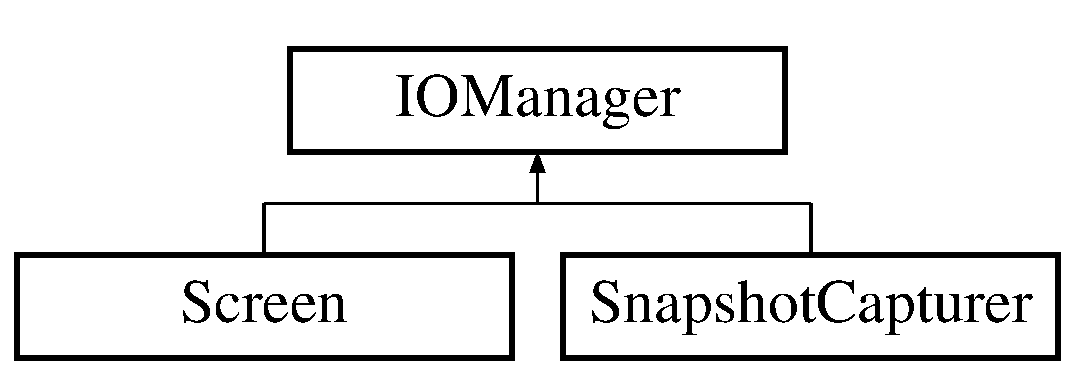
\includegraphics[height=2.000000cm]{class_i_o_manager}
\end{center}
\end{figure}
\subsection*{Public Member Functions}
\begin{DoxyCompactItemize}
\item 
void \hyperlink{class_i_o_manager_a996088d522ece770be55b53ec6fbde24}{Print\+Matrix} (const \hyperlink{class_matrix}{Matrix} \&)
\begin{DoxyCompactList}\small\item\em Mencetak sebuah matriks ke layar. \end{DoxyCompactList}\item 
void \hyperlink{class_i_o_manager_acef10db057340616aba5d0bb13142228}{Print\+World\+Map} ()
\begin{DoxyCompactList}\small\item\em Mencetak dunia beserta isinya. \end{DoxyCompactList}\end{DoxyCompactItemize}


\subsection{Detailed Description}
Abstract Base Class yang merupakan kelas dasar Input/\+Output. 

Kelas \hyperlink{class_i_o_manager}{I\+O\+Manager} bertanggung jawab untuk melakukan operasi-\/operasi Input/\+Output. \begin{DoxyAuthor}{Author}
Robert Sebastian Herlim 
\end{DoxyAuthor}
\begin{DoxyDate}{Date}
Maret 2016 
\end{DoxyDate}


\subsection{Member Function Documentation}
\index{I\+O\+Manager@{I\+O\+Manager}!Print\+Matrix@{Print\+Matrix}}
\index{Print\+Matrix@{Print\+Matrix}!I\+O\+Manager@{I\+O\+Manager}}
\subsubsection[{\texorpdfstring{Print\+Matrix(const Matrix \&)}{PrintMatrix(const Matrix &)}}]{\setlength{\rightskip}{0pt plus 5cm}void I\+O\+Manager\+::\+Print\+Matrix (
\begin{DoxyParamCaption}
\item[{const {\bf Matrix} \&}]{M}
\end{DoxyParamCaption}
)}\hypertarget{class_i_o_manager_a996088d522ece770be55b53ec6fbde24}{}\label{class_i_o_manager_a996088d522ece770be55b53ec6fbde24}


Mencetak sebuah matriks ke layar. 

Mencetak sebuah matriks ke layar \begin{DoxyReturn}{Returns}
void 
\end{DoxyReturn}
\index{I\+O\+Manager@{I\+O\+Manager}!Print\+World\+Map@{Print\+World\+Map}}
\index{Print\+World\+Map@{Print\+World\+Map}!I\+O\+Manager@{I\+O\+Manager}}
\subsubsection[{\texorpdfstring{Print\+World\+Map()}{PrintWorldMap()}}]{\setlength{\rightskip}{0pt plus 5cm}void I\+O\+Manager\+::\+Print\+World\+Map (
\begin{DoxyParamCaption}
{}
\end{DoxyParamCaption}
)}\hypertarget{class_i_o_manager_acef10db057340616aba5d0bb13142228}{}\label{class_i_o_manager_acef10db057340616aba5d0bb13142228}


Mencetak dunia beserta isinya. 

Mencetak sebuah state dunia beserta pada waktu tertentu dengan makhluk-\/makhluk yang ada di dalamnya ke layar \begin{DoxyReturn}{Returns}
void 
\end{DoxyReturn}


The documentation for this class was generated from the following files\+:\begin{DoxyCompactItemize}
\item 
C\+:/\+Users/\+Ngiong/\+Documents/\+Git\+Hub/\+Tubes\+Makhluk/v3/header/I\+O\+Manager.\+h\item 
C\+:/\+Users/\+Ngiong/\+Documents/\+Git\+Hub/\+Tubes\+Makhluk/v3/implementation/I\+O\+Manager.\+cpp\end{DoxyCompactItemize}

\hypertarget{class_keypress_handler}{}\section{Keypress\+Handler Class Reference}
\label{class_keypress_handler}\index{Keypress\+Handler@{Keypress\+Handler}}


Handler untuk masukan dari user berupa keypress.  




{\ttfamily \#include $<$Keypress\+Handler.\+h$>$}

\subsection*{Public Member Functions}
\begin{DoxyCompactItemize}
\item 
char \hyperlink{class_keypress_handler_acafd4a446c38d483d5bcbf758223965b}{get\+Last\+Keypress} ()
\begin{DoxyCompactList}\small\item\em Get Last Keypress. \end{DoxyCompactList}\item 
void \hyperlink{class_keypress_handler_a2a797123df099db8277254a9b864f6e0}{get\+Keypress} ()
\begin{DoxyCompactList}\small\item\em Prosedur untuk menerima keypress. \end{DoxyCompactList}\item 
void \hyperlink{class_keypress_handler_a519d07b7795f7efbea96a5b35ceb90ff}{do\+Action} ()
\begin{DoxyCompactList}\small\item\em Prosedur untuk menjalankan aksi dari keypress. \end{DoxyCompactList}\end{DoxyCompactItemize}
\subsection*{Static Public Member Functions}
\begin{DoxyCompactItemize}
\item 
static \hyperlink{class_keypress_handler}{Keypress\+Handler} $\ast$ \hyperlink{class_keypress_handler_a1c8568970784217a612470d9713bcbeb}{get\+Handler\+Instance} ()
\begin{DoxyCompactList}\small\item\em Get Singleton Instance dari kelas \hyperlink{class_keypress_handler}{Keypress\+Handler}. \end{DoxyCompactList}\item 
static void \hyperlink{class_keypress_handler_adfb5ff6e1aa6d4c3692d6097c2fbbe72}{Handle\+Keypress} ()
\begin{DoxyCompactList}\small\item\em Prosedur untuk menangani keypress. \end{DoxyCompactList}\end{DoxyCompactItemize}


\subsection{Detailed Description}
Handler untuk masukan dari user berupa keypress. 

Kelas \hyperlink{class_keypress_handler}{Keypress\+Handler} merupakan kelas yang berfungsi untuk menangani keypress yang dimasukkan oleh user \begin{DoxyAuthor}{Author}
Robert Sebastian Herlim 
\end{DoxyAuthor}
\begin{DoxyDate}{Date}
Maret 2016 
\end{DoxyDate}


\subsection{Member Function Documentation}
\index{Keypress\+Handler@{Keypress\+Handler}!do\+Action@{do\+Action}}
\index{do\+Action@{do\+Action}!Keypress\+Handler@{Keypress\+Handler}}
\subsubsection[{\texorpdfstring{do\+Action()}{doAction()}}]{\setlength{\rightskip}{0pt plus 5cm}void Keypress\+Handler\+::do\+Action (
\begin{DoxyParamCaption}
{}
\end{DoxyParamCaption}
)}\hypertarget{class_keypress_handler_a519d07b7795f7efbea96a5b35ceb90ff}{}\label{class_keypress_handler_a519d07b7795f7efbea96a5b35ceb90ff}


Prosedur untuk menjalankan aksi dari keypress. 

Melakukan aksi-\/aksi yang sesuai dengan karakter last\+Keypress yang tersimpan dalam instance \hyperlink{class_keypress_handler}{Keypress\+Handler} \begin{DoxyReturn}{Returns}
void 
\end{DoxyReturn}
\index{Keypress\+Handler@{Keypress\+Handler}!get\+Handler\+Instance@{get\+Handler\+Instance}}
\index{get\+Handler\+Instance@{get\+Handler\+Instance}!Keypress\+Handler@{Keypress\+Handler}}
\subsubsection[{\texorpdfstring{get\+Handler\+Instance()}{getHandlerInstance()}}]{\setlength{\rightskip}{0pt plus 5cm}static {\bf Keypress\+Handler}$\ast$ Keypress\+Handler\+::get\+Handler\+Instance (
\begin{DoxyParamCaption}
{}
\end{DoxyParamCaption}
)\hspace{0.3cm}{\ttfamily [inline]}, {\ttfamily [static]}}\hypertarget{class_keypress_handler_a1c8568970784217a612470d9713bcbeb}{}\label{class_keypress_handler_a1c8568970784217a612470d9713bcbeb}


Get Singleton Instance dari kelas \hyperlink{class_keypress_handler}{Keypress\+Handler}. 

Mengembalikan pointer dari objek kelas singleton pada kelas \hyperlink{class_keypress_handler}{Keypress\+Handler} \begin{DoxyReturn}{Returns}
pointer yang menunjuk ke singleton instance pada kelas \hyperlink{class_keypress_handler}{Keypress\+Handler} 
\end{DoxyReturn}
\index{Keypress\+Handler@{Keypress\+Handler}!get\+Keypress@{get\+Keypress}}
\index{get\+Keypress@{get\+Keypress}!Keypress\+Handler@{Keypress\+Handler}}
\subsubsection[{\texorpdfstring{get\+Keypress()}{getKeypress()}}]{\setlength{\rightskip}{0pt plus 5cm}void Keypress\+Handler\+::get\+Keypress (
\begin{DoxyParamCaption}
{}
\end{DoxyParamCaption}
)}\hypertarget{class_keypress_handler_a2a797123df099db8277254a9b864f6e0}{}\label{class_keypress_handler_a2a797123df099db8277254a9b864f6e0}


Prosedur untuk menerima keypress. 

Menunggu pengguna menekan tombol, serta mengubah karakter last\+Keypress yang tersimpan dalam instance \hyperlink{class_keypress_handler}{Keypress\+Handler} \begin{DoxyReturn}{Returns}
void 
\end{DoxyReturn}
\index{Keypress\+Handler@{Keypress\+Handler}!get\+Last\+Keypress@{get\+Last\+Keypress}}
\index{get\+Last\+Keypress@{get\+Last\+Keypress}!Keypress\+Handler@{Keypress\+Handler}}
\subsubsection[{\texorpdfstring{get\+Last\+Keypress()}{getLastKeypress()}}]{\setlength{\rightskip}{0pt plus 5cm}char Keypress\+Handler\+::get\+Last\+Keypress (
\begin{DoxyParamCaption}
{}
\end{DoxyParamCaption}
)\hspace{0.3cm}{\ttfamily [inline]}}\hypertarget{class_keypress_handler_acafd4a446c38d483d5bcbf758223965b}{}\label{class_keypress_handler_acafd4a446c38d483d5bcbf758223965b}


Get Last Keypress. 

Mengembalikan karakter yang terakhir ditekan oleh pengguna yang disimpan dalam instance \hyperlink{class_keypress_handler}{Keypress\+Handler} \begin{DoxyReturn}{Returns}
karakter yang terakhir ditekan pengguna 
\end{DoxyReturn}
\index{Keypress\+Handler@{Keypress\+Handler}!Handle\+Keypress@{Handle\+Keypress}}
\index{Handle\+Keypress@{Handle\+Keypress}!Keypress\+Handler@{Keypress\+Handler}}
\subsubsection[{\texorpdfstring{Handle\+Keypress()}{HandleKeypress()}}]{\setlength{\rightskip}{0pt plus 5cm}void Keypress\+Handler\+::\+Handle\+Keypress (
\begin{DoxyParamCaption}
{}
\end{DoxyParamCaption}
)\hspace{0.3cm}{\ttfamily [static]}}\hypertarget{class_keypress_handler_adfb5ff6e1aa6d4c3692d6097c2fbbe72}{}\label{class_keypress_handler_adfb5ff6e1aa6d4c3692d6097c2fbbe72}


Prosedur untuk menangani keypress. 

Menangani keypress dengan menunggu pengguna menekan tombol, dan melakukan aksi untuk karakter tersebut \begin{DoxyReturn}{Returns}
void 
\end{DoxyReturn}


The documentation for this class was generated from the following files\+:\begin{DoxyCompactItemize}
\item 
C\+:/\+Users/\+Ngiong/\+Documents/\+Git\+Hub/\+Tubes\+Makhluk/header/Keypress\+Handler.\+h\item 
C\+:/\+Users/\+Ngiong/\+Documents/\+Git\+Hub/\+Tubes\+Makhluk/implementation/Keypress\+Handler.\+cpp\end{DoxyCompactItemize}

\hypertarget{class_l_makhluk}{}\section{L\+Makhluk Class Reference}
\label{class_l_makhluk}\index{L\+Makhluk@{L\+Makhluk}}


List of makhluk.  




{\ttfamily \#include $<$L\+Makhluk.\+h$>$}

\subsection*{Public Member Functions}
\begin{DoxyCompactItemize}
\item 
\hyperlink{class_l_makhluk_a93e97387f0cdfa01c31d42832011180c}{L\+Makhluk} ()
\begin{DoxyCompactList}\small\item\em Constructor. \end{DoxyCompactList}\item 
\hyperlink{class_l_makhluk_ab02db38f176572e290cfb444862f96f2}{$\sim$\+L\+Makhluk} ()
\begin{DoxyCompactList}\small\item\em Destructor. \end{DoxyCompactList}\item 
void \hyperlink{class_l_makhluk_ab2d61c43b62e8574b36f486c8907b620}{Add} (\hyperlink{class_makhluk}{Makhluk} $\ast$)
\begin{DoxyCompactList}\small\item\em Menambah element pada list of makhluk. \end{DoxyCompactList}\item 
void \hyperlink{class_l_makhluk_a04f838bb55f2af5c0c3a0068ce21b4ff}{Del} (\hyperlink{class_makhluk}{Makhluk} $\ast$)
\begin{DoxyCompactList}\small\item\em Menghapus element pada list of makhluk. \end{DoxyCompactList}\item 
Elmt\+Makhluk $\ast$ \hyperlink{class_l_makhluk_a0ea8a32be37178cd38e3e2e0ac22d5ee}{get\+First} ()
\begin{DoxyCompactList}\small\item\em Get first element. \end{DoxyCompactList}\item 
void \hyperlink{class_l_makhluk_a4c1e3394813fb95f8850e3f3fe7d9cec}{set\+First} (Elmt\+Makhluk $\ast$\+\_\+first)
\begin{DoxyCompactList}\small\item\em Set first element. \end{DoxyCompactList}\item 
int \hyperlink{class_l_makhluk_a4ce8d0f4664716ac5237c2bd5bf0463e}{is\+Empty} ()
\begin{DoxyCompactList}\small\item\em Fungsi untuk mengecek apakah sebuah list kosong. \end{DoxyCompactList}\item 
Elmt\+Makhluk $\ast$ \hyperlink{class_l_makhluk_ac7bd40c1c06471b82f125000efa92add}{get\+Last} ()
\begin{DoxyCompactList}\small\item\em Get last element. \end{DoxyCompactList}\item 
Elmt\+Makhluk $\ast$ \hyperlink{class_l_makhluk_a11328333ff18d44b56eb3ff917340f64}{find\+Prec\+Makhluk} (\hyperlink{class_makhluk}{Makhluk} $\ast$)
\begin{DoxyCompactList}\small\item\em Mencari element sebelum sebuah makhluk. \end{DoxyCompactList}\item 
Elmt\+Makhluk $\ast$ \hyperlink{class_l_makhluk_a41073415d0c395c915ba47099aba7d69}{find\+Makhluk} (\hyperlink{class_makhluk}{Makhluk} $\ast$)
\begin{DoxyCompactList}\small\item\em Mencari sebuah makhluk. \end{DoxyCompactList}\end{DoxyCompactItemize}


\subsection{Detailed Description}
List of makhluk. 

Menciptakan list of makhluk \begin{DoxyAuthor}{Author}
Micky Yudi Utama 
\end{DoxyAuthor}
\begin{DoxyDate}{Date}
Maret 2016 
\end{DoxyDate}


\subsection{Constructor \& Destructor Documentation}
\index{L\+Makhluk@{L\+Makhluk}!L\+Makhluk@{L\+Makhluk}}
\index{L\+Makhluk@{L\+Makhluk}!L\+Makhluk@{L\+Makhluk}}
\subsubsection[{\texorpdfstring{L\+Makhluk()}{LMakhluk()}}]{\setlength{\rightskip}{0pt plus 5cm}L\+Makhluk\+::\+L\+Makhluk (
\begin{DoxyParamCaption}
{}
\end{DoxyParamCaption}
)}\hypertarget{class_l_makhluk_a93e97387f0cdfa01c31d42832011180c}{}\label{class_l_makhluk_a93e97387f0cdfa01c31d42832011180c}


Constructor. 

Menciptakan sebuah list of makhluk \index{L\+Makhluk@{L\+Makhluk}!````~L\+Makhluk@{$\sim$\+L\+Makhluk}}
\index{````~L\+Makhluk@{$\sim$\+L\+Makhluk}!L\+Makhluk@{L\+Makhluk}}
\subsubsection[{\texorpdfstring{$\sim$\+L\+Makhluk()}{~LMakhluk()}}]{\setlength{\rightskip}{0pt plus 5cm}L\+Makhluk\+::$\sim$\+L\+Makhluk (
\begin{DoxyParamCaption}
{}
\end{DoxyParamCaption}
)}\hypertarget{class_l_makhluk_ab02db38f176572e290cfb444862f96f2}{}\label{class_l_makhluk_ab02db38f176572e290cfb444862f96f2}


Destructor. 

Menghapus list of makhluk 

\subsection{Member Function Documentation}
\index{L\+Makhluk@{L\+Makhluk}!Add@{Add}}
\index{Add@{Add}!L\+Makhluk@{L\+Makhluk}}
\subsubsection[{\texorpdfstring{Add(\+Makhluk $\ast$)}{Add(Makhluk *)}}]{\setlength{\rightskip}{0pt plus 5cm}void L\+Makhluk\+::\+Add (
\begin{DoxyParamCaption}
\item[{{\bf Makhluk} $\ast$}]{M}
\end{DoxyParamCaption}
)}\hypertarget{class_l_makhluk_ab2d61c43b62e8574b36f486c8907b620}{}\label{class_l_makhluk_ab2d61c43b62e8574b36f486c8907b620}


Menambah element pada list of makhluk. 

Menambah element pada bagian belakang list of makhluk 
\begin{DoxyParams}{Parameters}
{\em M} & Makhluk$\ast$ \hyperlink{class_makhluk}{Makhluk} yang akan ditambah ke list \\
\hline
\end{DoxyParams}
\begin{DoxyReturn}{Returns}
void 
\end{DoxyReturn}
\index{L\+Makhluk@{L\+Makhluk}!Del@{Del}}
\index{Del@{Del}!L\+Makhluk@{L\+Makhluk}}
\subsubsection[{\texorpdfstring{Del(\+Makhluk $\ast$)}{Del(Makhluk *)}}]{\setlength{\rightskip}{0pt plus 5cm}void L\+Makhluk\+::\+Del (
\begin{DoxyParamCaption}
\item[{{\bf Makhluk} $\ast$}]{M}
\end{DoxyParamCaption}
)}\hypertarget{class_l_makhluk_a04f838bb55f2af5c0c3a0068ce21b4ff}{}\label{class_l_makhluk_a04f838bb55f2af5c0c3a0068ce21b4ff}


Menghapus element pada list of makhluk. 

Menghapus makhluk M pada list of makhluk 
\begin{DoxyParams}{Parameters}
{\em M} & Makhluk$\ast$ \hyperlink{class_makhluk}{Makhluk} yang akan dihapus dari list \\
\hline
\end{DoxyParams}
\begin{DoxyReturn}{Returns}
void 
\end{DoxyReturn}
\index{L\+Makhluk@{L\+Makhluk}!find\+Makhluk@{find\+Makhluk}}
\index{find\+Makhluk@{find\+Makhluk}!L\+Makhluk@{L\+Makhluk}}
\subsubsection[{\texorpdfstring{find\+Makhluk(\+Makhluk $\ast$)}{findMakhluk(Makhluk *)}}]{\setlength{\rightskip}{0pt plus 5cm}L\+Makhluk\+::\+Elmt\+Makhluk $\ast$ L\+Makhluk\+::find\+Makhluk (
\begin{DoxyParamCaption}
\item[{{\bf Makhluk} $\ast$}]{M}
\end{DoxyParamCaption}
)}\hypertarget{class_l_makhluk_a41073415d0c395c915ba47099aba7d69}{}\label{class_l_makhluk_a41073415d0c395c915ba47099aba7d69}


Mencari sebuah makhluk. 

Mencari sebuah makhluk pada list of makhluk 
\begin{DoxyParams}{Parameters}
{\em M} & Makhluk$\ast$ \hyperlink{class_makhluk}{Makhluk} yang akan dicari \\
\hline
\end{DoxyParams}
\begin{DoxyReturn}{Returns}
\hyperlink{class_makhluk}{Makhluk} 
\end{DoxyReturn}
\index{L\+Makhluk@{L\+Makhluk}!find\+Prec\+Makhluk@{find\+Prec\+Makhluk}}
\index{find\+Prec\+Makhluk@{find\+Prec\+Makhluk}!L\+Makhluk@{L\+Makhluk}}
\subsubsection[{\texorpdfstring{find\+Prec\+Makhluk(\+Makhluk $\ast$)}{findPrecMakhluk(Makhluk *)}}]{\setlength{\rightskip}{0pt plus 5cm}L\+Makhluk\+::\+Elmt\+Makhluk $\ast$ L\+Makhluk\+::find\+Prec\+Makhluk (
\begin{DoxyParamCaption}
\item[{{\bf Makhluk} $\ast$}]{M}
\end{DoxyParamCaption}
)}\hypertarget{class_l_makhluk_a11328333ff18d44b56eb3ff917340f64}{}\label{class_l_makhluk_a11328333ff18d44b56eb3ff917340f64}


Mencari element sebelum sebuah makhluk. 

Mencari element sebelum sebuah makhluk pada list of makhluk 
\begin{DoxyParams}{Parameters}
{\em M} & Makhluk$\ast$ \hyperlink{class_makhluk}{Makhluk} yang akan dicari element sebelumnya \\
\hline
\end{DoxyParams}
\begin{DoxyReturn}{Returns}
Element sebelum makhluk M 
\end{DoxyReturn}
\index{L\+Makhluk@{L\+Makhluk}!get\+First@{get\+First}}
\index{get\+First@{get\+First}!L\+Makhluk@{L\+Makhluk}}
\subsubsection[{\texorpdfstring{get\+First()}{getFirst()}}]{\setlength{\rightskip}{0pt plus 5cm}Elmt\+Makhluk$\ast$ L\+Makhluk\+::get\+First (
\begin{DoxyParamCaption}
{}
\end{DoxyParamCaption}
)\hspace{0.3cm}{\ttfamily [inline]}}\hypertarget{class_l_makhluk_a0ea8a32be37178cd38e3e2e0ac22d5ee}{}\label{class_l_makhluk_a0ea8a32be37178cd38e3e2e0ac22d5ee}


Get first element. 

Mengambil first element dari list of makhluk \begin{DoxyReturn}{Returns}
First element 
\end{DoxyReturn}
\index{L\+Makhluk@{L\+Makhluk}!get\+Last@{get\+Last}}
\index{get\+Last@{get\+Last}!L\+Makhluk@{L\+Makhluk}}
\subsubsection[{\texorpdfstring{get\+Last()}{getLast()}}]{\setlength{\rightskip}{0pt plus 5cm}L\+Makhluk\+::\+Elmt\+Makhluk $\ast$ L\+Makhluk\+::get\+Last (
\begin{DoxyParamCaption}
{}
\end{DoxyParamCaption}
)}\hypertarget{class_l_makhluk_ac7bd40c1c06471b82f125000efa92add}{}\label{class_l_makhluk_ac7bd40c1c06471b82f125000efa92add}


Get last element. 

Mengambul last element dari list of makhluk \begin{DoxyReturn}{Returns}
Last element 
\end{DoxyReturn}
\index{L\+Makhluk@{L\+Makhluk}!is\+Empty@{is\+Empty}}
\index{is\+Empty@{is\+Empty}!L\+Makhluk@{L\+Makhluk}}
\subsubsection[{\texorpdfstring{is\+Empty()}{isEmpty()}}]{\setlength{\rightskip}{0pt plus 5cm}int L\+Makhluk\+::is\+Empty (
\begin{DoxyParamCaption}
{}
\end{DoxyParamCaption}
)\hspace{0.3cm}{\ttfamily [inline]}}\hypertarget{class_l_makhluk_a4ce8d0f4664716ac5237c2bd5bf0463e}{}\label{class_l_makhluk_a4ce8d0f4664716ac5237c2bd5bf0463e}


Fungsi untuk mengecek apakah sebuah list kosong. 

Mengembalikan 0 jika list kosong, 1 jika list tidak kosong \begin{DoxyReturn}{Returns}
Bilangan bulat 0 atau 1 
\end{DoxyReturn}
\index{L\+Makhluk@{L\+Makhluk}!set\+First@{set\+First}}
\index{set\+First@{set\+First}!L\+Makhluk@{L\+Makhluk}}
\subsubsection[{\texorpdfstring{set\+First(\+Elmt\+Makhluk $\ast$\+\_\+first)}{setFirst(ElmtMakhluk *_first)}}]{\setlength{\rightskip}{0pt plus 5cm}void L\+Makhluk\+::set\+First (
\begin{DoxyParamCaption}
\item[{Elmt\+Makhluk $\ast$}]{\+\_\+first}
\end{DoxyParamCaption}
)\hspace{0.3cm}{\ttfamily [inline]}}\hypertarget{class_l_makhluk_a4c1e3394813fb95f8850e3f3fe7d9cec}{}\label{class_l_makhluk_a4c1e3394813fb95f8850e3f3fe7d9cec}


Set first element. 

Mengassign first element list berdasarkan parameter 
\begin{DoxyParams}{Parameters}
{\em \+\_\+first} & Elmt\+Makhluk$\ast$ First element dari list of makhluk \\
\hline
\end{DoxyParams}
\begin{DoxyReturn}{Returns}
void 
\end{DoxyReturn}


The documentation for this class was generated from the following files\+:\begin{DoxyCompactItemize}
\item 
C\+:/\+Users/\+Ngiong/\+Documents/\+Git\+Hub/\+Tubes\+Makhluk/header/L\+Makhluk.\+h\item 
C\+:/\+Users/\+Ngiong/\+Documents/\+Git\+Hub/\+Tubes\+Makhluk/implementation/L\+Makhluk.\+cpp\end{DoxyCompactItemize}

\hypertarget{class_makhluk}{}\section{Makhluk Class Reference}
\label{class_makhluk}\index{Makhluk@{Makhluk}}
Inheritance diagram for Makhluk\+:\begin{figure}[H]
\begin{center}
\leavevmode
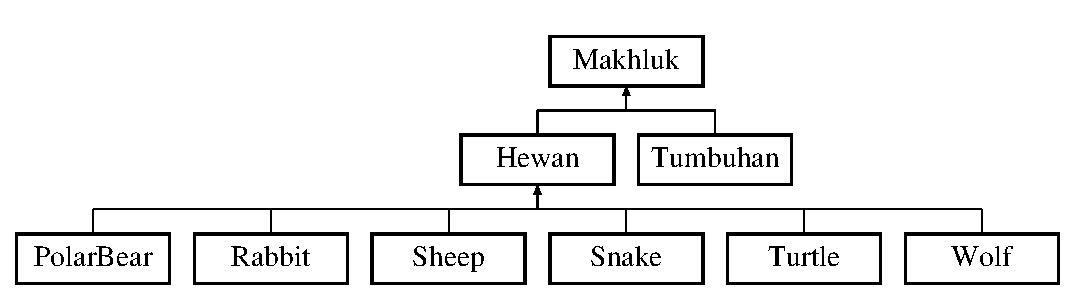
\includegraphics[height=3.000000cm]{class_makhluk}
\end{center}
\end{figure}
\subsection*{Public Member Functions}
\begin{DoxyCompactItemize}
\item 
char {\bfseries get\+ID} () const \hypertarget{class_makhluk_ac1c4f42107c702ba928188fa2530c5f3}{}\label{class_makhluk_ac1c4f42107c702ba928188fa2530c5f3}

\item 
int {\bfseries get\+Age} () const \hypertarget{class_makhluk_aba388ab8fe2eafcda3495d16b7c9e4b7}{}\label{class_makhluk_aba388ab8fe2eafcda3495d16b7c9e4b7}

\item 
int {\bfseries get\+Max\+Age} () const \hypertarget{class_makhluk_ae002b2faad22dc950a3f42bd62ea54d9}{}\label{class_makhluk_ae002b2faad22dc950a3f42bd62ea54d9}

\item 
\hyperlink{class_point}{Point} {\bfseries get\+Position} () const \hypertarget{class_makhluk_a451445ffca2c8c3e45800b7096e65239}{}\label{class_makhluk_a451445ffca2c8c3e45800b7096e65239}

\item 
void {\bfseries set\+Position} (const \hyperlink{class_point}{Point} \&P)\hypertarget{class_makhluk_a7abec2f20a8c601ec6042682264a7f64}{}\label{class_makhluk_a7abec2f20a8c601ec6042682264a7f64}

\item 
virtual void {\bfseries Live} ()=0\hypertarget{class_makhluk_af0cc274cef5058743f6b048a78843bd1}{}\label{class_makhluk_af0cc274cef5058743f6b048a78843bd1}

\item 
int {\bfseries is\+Alive} ()\hypertarget{class_makhluk_a1677bd235210d490951fcd8a5653160d}{}\label{class_makhluk_a1677bd235210d490951fcd8a5653160d}

\item 
void {\bfseries Kill} ()\hypertarget{class_makhluk_a8031caebf761dbc200430c24726ca339}{}\label{class_makhluk_a8031caebf761dbc200430c24726ca339}

\end{DoxyCompactItemize}
\subsection*{Static Public Member Functions}
\begin{DoxyCompactItemize}
\item 
static void {\bfseries Make\+Alive} (\hyperlink{class_makhluk}{Makhluk} $\ast$)\hypertarget{class_makhluk_a46b686a6f1533958650a60e3d7268b99}{}\label{class_makhluk_a46b686a6f1533958650a60e3d7268b99}

\end{DoxyCompactItemize}
\subsection*{Protected Member Functions}
\begin{DoxyCompactItemize}
\item 
{\bfseries Makhluk} (char, int)\hypertarget{class_makhluk_afd36e7fe75e525a38d5cfc8a1e6b48be}{}\label{class_makhluk_afd36e7fe75e525a38d5cfc8a1e6b48be}

\end{DoxyCompactItemize}
\subsection*{Protected Attributes}
\begin{DoxyCompactItemize}
\item 
const char {\bfseries ID}\hypertarget{class_makhluk_a287dd5d101d81990399f00f4a77a36f5}{}\label{class_makhluk_a287dd5d101d81990399f00f4a77a36f5}

\item 
const int {\bfseries max\+Age}\hypertarget{class_makhluk_a50350ef02b62af484c769b8118f8c4ae}{}\label{class_makhluk_a50350ef02b62af484c769b8118f8c4ae}

\item 
int {\bfseries age}\hypertarget{class_makhluk_aacf25b9c59e644e709b730f5239996f6}{}\label{class_makhluk_aacf25b9c59e644e709b730f5239996f6}

\item 
int {\bfseries status}\hypertarget{class_makhluk_aa3eefed357a56f6b86f0080083d91d31}{}\label{class_makhluk_aa3eefed357a56f6b86f0080083d91d31}

\item 
\hyperlink{class_point}{Point} {\bfseries pos}\hypertarget{class_makhluk_a920e46e39a404909a292802669bed0c2}{}\label{class_makhluk_a920e46e39a404909a292802669bed0c2}

\end{DoxyCompactItemize}


The documentation for this class was generated from the following files\+:\begin{DoxyCompactItemize}
\item 
C\+:/\+Users/\+Ngiong/\+Documents/\+Git\+Hub/\+Tubes\+Makhluk/header/Makhluk.\+h\item 
C\+:/\+Users/\+Ngiong/\+Documents/\+Git\+Hub/\+Tubes\+Makhluk/implementation/Makhluk.\+cpp\end{DoxyCompactItemize}

\hypertarget{class_matrix}{}\section{Matrix Class Reference}
\label{class_matrix}\index{Matrix@{Matrix}}


Representasi array dua dimensi.  




{\ttfamily \#include $<$Matrix.\+h$>$}

\subsection*{Public Member Functions}
\begin{DoxyCompactItemize}
\item 
\hyperlink{class_matrix_adfbeb67cc3c43d96c53f881d79f919cb}{Matrix} (int, int)
\begin{DoxyCompactList}\small\item\em Constructor. \end{DoxyCompactList}\item 
\hyperlink{class_matrix_a0b9cfa2302a0273afb1b26e501f93abc}{Matrix} (const \hyperlink{class_matrix}{Matrix} \&)
\begin{DoxyCompactList}\small\item\em Copy Constructor. \end{DoxyCompactList}\item 
\hyperlink{class_matrix_a9b1c3627f573d78a2f08623fdfef990f}{$\sim$\+Matrix} ()
\begin{DoxyCompactList}\small\item\em Destructor. \end{DoxyCompactList}\item 
int \hyperlink{class_matrix_a518609c744a502753d79063d75075312}{get\+N\+Brs} () const 
\begin{DoxyCompactList}\small\item\em Get jumlah baris. \end{DoxyCompactList}\item 
int \hyperlink{class_matrix_a9d540e5e85c41e7852308b1000a04ecd}{get\+N\+Kol} () const 
\begin{DoxyCompactList}\small\item\em Get jumlah kolom. \end{DoxyCompactList}\item 
char \hyperlink{class_matrix_a58e92d242a032a24ebbbfb235093edd9}{get\+Info} (int i, int j) const 
\begin{DoxyCompactList}\small\item\em Get nilai sebuah elemen matriks. \end{DoxyCompactList}\item 
void \hyperlink{class_matrix_adf43d84e79f4d48bdd087c3af5099a0b}{set\+Info} (char c, int i, int j)
\begin{DoxyCompactList}\small\item\em Setter nilai sebuah elemen matriks. \end{DoxyCompactList}\end{DoxyCompactItemize}


\subsection{Detailed Description}
Representasi array dua dimensi. 

Kelas Matriks berisi sejumlah elemen karakter yang akan digunakan untuk menampilkan state dunia pada layar. \begin{DoxyAuthor}{Author}
Robert Sebastian Herlim 
\end{DoxyAuthor}
\begin{DoxyDate}{Date}
Maret 2016 
\end{DoxyDate}


\subsection{Constructor \& Destructor Documentation}
\index{Matrix@{Matrix}!Matrix@{Matrix}}
\index{Matrix@{Matrix}!Matrix@{Matrix}}
\subsubsection[{\texorpdfstring{Matrix(int, int)}{Matrix(int, int)}}]{\setlength{\rightskip}{0pt plus 5cm}Matrix\+::\+Matrix (
\begin{DoxyParamCaption}
\item[{int}]{\+\_\+\+N\+Brs, }
\item[{int}]{\+\_\+\+N\+Kol}
\end{DoxyParamCaption}
)}\hypertarget{class_matrix_adfbeb67cc3c43d96c53f881d79f919cb}{}\label{class_matrix_adfbeb67cc3c43d96c53f881d79f919cb}


Constructor. 

Menciptakan sebuah matriks dengan ukuran yang di-\/pass melalui parameter. Matriks yang tercipta akan terisi karakter \textquotesingle{}\#\textquotesingle{} di bagian tepi matriks sebagai border, dan \textquotesingle{}.\textquotesingle{} pada bagian dalamnya. 
\begin{DoxyParams}{Parameters}
{\em \+\_\+\+N\+Brs} & int jumlah baris \\
\hline
{\em \+\_\+\+N\+Kol} & int jumlah kolom \\
\hline
\end{DoxyParams}
\index{Matrix@{Matrix}!Matrix@{Matrix}}
\index{Matrix@{Matrix}!Matrix@{Matrix}}
\subsubsection[{\texorpdfstring{Matrix(const Matrix \&)}{Matrix(const Matrix &)}}]{\setlength{\rightskip}{0pt plus 5cm}Matrix\+::\+Matrix (
\begin{DoxyParamCaption}
\item[{const {\bf Matrix} \&}]{Mat}
\end{DoxyParamCaption}
)}\hypertarget{class_matrix_a0b9cfa2302a0273afb1b26e501f93abc}{}\label{class_matrix_a0b9cfa2302a0273afb1b26e501f93abc}


Copy Constructor. 

Menciptakan sebuah matriks yang merupakan salinan dari matriks lain. Matriks yang tercipta akan terisi karakter \textquotesingle{}\#\textquotesingle{} di bagian tepi matriks sebagai border, dan \textquotesingle{}.\textquotesingle{} pada bagian dalamnya. 
\begin{DoxyParams}{Parameters}
{\em Mat} & const \hyperlink{class_matrix}{Matrix}\& Matriks yang akan disalin \\
\hline
\end{DoxyParams}
\index{Matrix@{Matrix}!````~Matrix@{$\sim$\+Matrix}}
\index{````~Matrix@{$\sim$\+Matrix}!Matrix@{Matrix}}
\subsubsection[{\texorpdfstring{$\sim$\+Matrix()}{~Matrix()}}]{\setlength{\rightskip}{0pt plus 5cm}Matrix\+::$\sim$\+Matrix (
\begin{DoxyParamCaption}
{}
\end{DoxyParamCaption}
)}\hypertarget{class_matrix_a9b1c3627f573d78a2f08623fdfef990f}{}\label{class_matrix_a9b1c3627f573d78a2f08623fdfef990f}


Destructor. 

Memusnahkan sebuah matriks 

\subsection{Member Function Documentation}
\index{Matrix@{Matrix}!get\+Info@{get\+Info}}
\index{get\+Info@{get\+Info}!Matrix@{Matrix}}
\subsubsection[{\texorpdfstring{get\+Info(int i, int j) const }{getInfo(int i, int j) const }}]{\setlength{\rightskip}{0pt plus 5cm}char Matrix\+::get\+Info (
\begin{DoxyParamCaption}
\item[{int}]{i, }
\item[{int}]{j}
\end{DoxyParamCaption}
) const}\hypertarget{class_matrix_a58e92d242a032a24ebbbfb235093edd9}{}\label{class_matrix_a58e92d242a032a24ebbbfb235093edd9}


Get nilai sebuah elemen matriks. 

Mengambil nilai karakter yang tersimpan pada elemen matriks di baris ke-\/i dan kolom ke-\/j 
\begin{DoxyParams}{Parameters}
{\em i} & int Indeks baris elemen matriks \\
\hline
{\em j} & int Indeks kolom elemen matriks \\
\hline
\end{DoxyParams}
\begin{DoxyReturn}{Returns}
Karakter M\mbox{[}i\mbox{]}\mbox{[}j\mbox{]} 
\end{DoxyReturn}
\index{Matrix@{Matrix}!get\+N\+Brs@{get\+N\+Brs}}
\index{get\+N\+Brs@{get\+N\+Brs}!Matrix@{Matrix}}
\subsubsection[{\texorpdfstring{get\+N\+Brs() const }{getNBrs() const }}]{\setlength{\rightskip}{0pt plus 5cm}int Matrix\+::get\+N\+Brs (
\begin{DoxyParamCaption}
{}
\end{DoxyParamCaption}
) const\hspace{0.3cm}{\ttfamily [inline]}}\hypertarget{class_matrix_a518609c744a502753d79063d75075312}{}\label{class_matrix_a518609c744a502753d79063d75075312}


Get jumlah baris. 

Mengambil nilai N\+Brs, yaitu jumlah baris pada matriks \begin{DoxyReturn}{Returns}
Nilai konstanta N\+Brs 
\end{DoxyReturn}
\index{Matrix@{Matrix}!get\+N\+Kol@{get\+N\+Kol}}
\index{get\+N\+Kol@{get\+N\+Kol}!Matrix@{Matrix}}
\subsubsection[{\texorpdfstring{get\+N\+Kol() const }{getNKol() const }}]{\setlength{\rightskip}{0pt plus 5cm}int Matrix\+::get\+N\+Kol (
\begin{DoxyParamCaption}
{}
\end{DoxyParamCaption}
) const\hspace{0.3cm}{\ttfamily [inline]}}\hypertarget{class_matrix_a9d540e5e85c41e7852308b1000a04ecd}{}\label{class_matrix_a9d540e5e85c41e7852308b1000a04ecd}


Get jumlah kolom. 

Mengambil nilai N\+Kol, yaitu jumlah kolom pada matriks \begin{DoxyReturn}{Returns}
nilai konstanta N\+Kol 
\end{DoxyReturn}
\index{Matrix@{Matrix}!set\+Info@{set\+Info}}
\index{set\+Info@{set\+Info}!Matrix@{Matrix}}
\subsubsection[{\texorpdfstring{set\+Info(char c, int i, int j)}{setInfo(char c, int i, int j)}}]{\setlength{\rightskip}{0pt plus 5cm}void Matrix\+::set\+Info (
\begin{DoxyParamCaption}
\item[{char}]{c, }
\item[{int}]{i, }
\item[{int}]{j}
\end{DoxyParamCaption}
)}\hypertarget{class_matrix_adf43d84e79f4d48bdd087c3af5099a0b}{}\label{class_matrix_adf43d84e79f4d48bdd087c3af5099a0b}


Setter nilai sebuah elemen matriks. 

Melakukan assignment pada elemen matriks yang terletak di baris ke-\/i dan kolom ke-\/j 
\begin{DoxyParams}{Parameters}
{\em c} & char Nilai baru yang akan di-\/assign \\
\hline
{\em i} & int Indeks baris elemen matriks \\
\hline
{\em j} & int Indeks kolom elemen matriks \\
\hline
\end{DoxyParams}
\begin{DoxyReturn}{Returns}
void 
\end{DoxyReturn}


The documentation for this class was generated from the following files\+:\begin{DoxyCompactItemize}
\item 
C\+:/\+Users/\+Ngiong/\+Documents/\+Git\+Hub/\+Tubes\+Makhluk/header/Matrix.\+h\item 
C\+:/\+Users/\+Ngiong/\+Documents/\+Git\+Hub/\+Tubes\+Makhluk/implementation/Matrix.\+cpp\end{DoxyCompactItemize}

\hypertarget{class_point}{}\section{Point Class Reference}
\label{class_point}\index{Point@{Point}}


Representasi titik dalam koordinat kartesian.  




{\ttfamily \#include $<$Point.\+h$>$}

\subsection*{Public Member Functions}
\begin{DoxyCompactItemize}
\item 
\hyperlink{class_point_ad92f2337b839a94ce97dcdb439b4325a}{Point} ()
\begin{DoxyCompactList}\small\item\em Default Constructor. \end{DoxyCompactList}\item 
\hyperlink{class_point_a7e2f39fba71990705aac9ffee1b389b4}{Point} (int, int)
\begin{DoxyCompactList}\small\item\em Constructor. \end{DoxyCompactList}\item 
\hyperlink{class_point_a5b7ec0fb127734c1cd5c6f350a3990fc}{Point} (const \hyperlink{class_point}{Point} \&)
\begin{DoxyCompactList}\small\item\em Copy Constructor. \end{DoxyCompactList}\item 
int \hyperlink{class_point_a0b82a4aa9614c11854abc507d89a70a9}{getX} ()
\begin{DoxyCompactList}\small\item\em Get nilai absis. \end{DoxyCompactList}\item 
int \hyperlink{class_point_a3770f321c49dfe7ca463900fddc2e2bc}{getY} ()
\begin{DoxyCompactList}\small\item\em Get nilai ordinat. \end{DoxyCompactList}\item 
void \hyperlink{class_point_aa1d444024813ee4def15bb8576c351fc}{setX} (int \+\_\+x)
\begin{DoxyCompactList}\small\item\em Setter untuk nilai absis. \end{DoxyCompactList}\item 
void \hyperlink{class_point_aadbaf15691dc524ea45716ef3fa24285}{setY} (int \+\_\+y)
\begin{DoxyCompactList}\small\item\em Setter untuk nilai ordinat. \end{DoxyCompactList}\item 
void \hyperlink{class_point_ac6a31803b1aa63e55101c3e7ce6c2d4c}{increment} (int, int)
\begin{DoxyCompactList}\small\item\em Melakukan translasi point. \end{DoxyCompactList}\end{DoxyCompactItemize}
\subsection*{Static Public Member Functions}
\begin{DoxyCompactItemize}
\item 
static int \hyperlink{class_point_ae137261026b05d581d5afda0d3dbd752}{get\+Distance} (\hyperlink{class_point}{Point} \&, \hyperlink{class_point}{Point} \&)
\begin{DoxyCompactList}\small\item\em Menghitung jarak euclidean dari 2 buah point. \end{DoxyCompactList}\end{DoxyCompactItemize}


\subsection{Detailed Description}
Representasi titik dalam koordinat kartesian. 

Kelas \hyperlink{class_point}{Point} berisi dua buah bilangan bulat untuk merepresentasikan suatu koordinat kartesian \begin{DoxyAuthor}{Author}
Robert Sebastian Herlim 
\end{DoxyAuthor}
\begin{DoxyDate}{Date}
Maret 2016 
\end{DoxyDate}


\subsection{Constructor \& Destructor Documentation}
\index{Point@{Point}!Point@{Point}}
\index{Point@{Point}!Point@{Point}}
\subsubsection[{\texorpdfstring{Point()}{Point()}}]{\setlength{\rightskip}{0pt plus 5cm}Point\+::\+Point (
\begin{DoxyParamCaption}
{}
\end{DoxyParamCaption}
)}\hypertarget{class_point_ad92f2337b839a94ce97dcdb439b4325a}{}\label{class_point_ad92f2337b839a94ce97dcdb439b4325a}


Default Constructor. 

Menciptakan sebuah point dengan koordinat default. \index{Point@{Point}!Point@{Point}}
\index{Point@{Point}!Point@{Point}}
\subsubsection[{\texorpdfstring{Point(int, int)}{Point(int, int)}}]{\setlength{\rightskip}{0pt plus 5cm}Point\+::\+Point (
\begin{DoxyParamCaption}
\item[{int}]{\+\_\+x = {\ttfamily DEFAULT\+\_\+X}, }
\item[{int}]{\+\_\+y = {\ttfamily DEFAULT\+\_\+Y}}
\end{DoxyParamCaption}
)}\hypertarget{class_point_a7e2f39fba71990705aac9ffee1b389b4}{}\label{class_point_a7e2f39fba71990705aac9ffee1b389b4}


Constructor. 

Menciptakan sebuah point dengan koordinat yang di-\/passing melalui parameter. 
\begin{DoxyParams}{Parameters}
{\em \+\_\+x} & int Nilai absis point yang akan diciptakan \\
\hline
{\em \+\_\+y} & int Nilai ordinat point yang akan diciptakan \\
\hline
\end{DoxyParams}
\index{Point@{Point}!Point@{Point}}
\index{Point@{Point}!Point@{Point}}
\subsubsection[{\texorpdfstring{Point(const Point \&)}{Point(const Point &)}}]{\setlength{\rightskip}{0pt plus 5cm}Point\+::\+Point (
\begin{DoxyParamCaption}
\item[{const {\bf Point} \&}]{P}
\end{DoxyParamCaption}
)}\hypertarget{class_point_a5b7ec0fb127734c1cd5c6f350a3990fc}{}\label{class_point_a5b7ec0fb127734c1cd5c6f350a3990fc}


Copy Constructor. 

Menciptakan sebuah point dengan menyalin sebuah point yang sudah tercipta 
\begin{DoxyParams}{Parameters}
{\em P} & const \hyperlink{class_point}{Point}\& \hyperlink{class_point}{Point} yang akan disalin \\
\hline
\end{DoxyParams}


\subsection{Member Function Documentation}
\index{Point@{Point}!get\+Distance@{get\+Distance}}
\index{get\+Distance@{get\+Distance}!Point@{Point}}
\subsubsection[{\texorpdfstring{get\+Distance(\+Point \&, Point \&)}{getDistance(Point &, Point &)}}]{\setlength{\rightskip}{0pt plus 5cm}int Point\+::get\+Distance (
\begin{DoxyParamCaption}
\item[{{\bf Point} \&}]{P1, }
\item[{{\bf Point} \&}]{P2}
\end{DoxyParamCaption}
)\hspace{0.3cm}{\ttfamily [static]}}\hypertarget{class_point_ae137261026b05d581d5afda0d3dbd752}{}\label{class_point_ae137261026b05d581d5afda0d3dbd752}


Menghitung jarak euclidean dari 2 buah point. 

Menghitung jarak euclidean dari 2 buah point yang di-\/passing melalui parameter 
\begin{DoxyParams}{Parameters}
{\em P1} & \hyperlink{class_point}{Point} Titik pertama \\
\hline
{\em P2} & \hyperlink{class_point}{Point} Titik kedua \\
\hline
\end{DoxyParams}
\begin{DoxyReturn}{Returns}
Bilangan bulat yang merupakan jarak euclidean antara titik pertama dan titik kedua 
\end{DoxyReturn}
\index{Point@{Point}!getX@{getX}}
\index{getX@{getX}!Point@{Point}}
\subsubsection[{\texorpdfstring{get\+X()}{getX()}}]{\setlength{\rightskip}{0pt plus 5cm}int Point\+::getX (
\begin{DoxyParamCaption}
{}
\end{DoxyParamCaption}
)\hspace{0.3cm}{\ttfamily [inline]}}\hypertarget{class_point_a0b82a4aa9614c11854abc507d89a70a9}{}\label{class_point_a0b82a4aa9614c11854abc507d89a70a9}


Get nilai absis. 

Mengambil nilai absis dari point \begin{DoxyReturn}{Returns}
nilai absis dari point 
\end{DoxyReturn}
\index{Point@{Point}!getY@{getY}}
\index{getY@{getY}!Point@{Point}}
\subsubsection[{\texorpdfstring{get\+Y()}{getY()}}]{\setlength{\rightskip}{0pt plus 5cm}int Point\+::getY (
\begin{DoxyParamCaption}
{}
\end{DoxyParamCaption}
)\hspace{0.3cm}{\ttfamily [inline]}}\hypertarget{class_point_a3770f321c49dfe7ca463900fddc2e2bc}{}\label{class_point_a3770f321c49dfe7ca463900fddc2e2bc}


Get nilai ordinat. 

Mengambil nilai ordinat dari point \begin{DoxyReturn}{Returns}
nilai ordinat dari point 
\end{DoxyReturn}
\index{Point@{Point}!increment@{increment}}
\index{increment@{increment}!Point@{Point}}
\subsubsection[{\texorpdfstring{increment(int, int)}{increment(int, int)}}]{\setlength{\rightskip}{0pt plus 5cm}void Point\+::increment (
\begin{DoxyParamCaption}
\item[{int}]{dx, }
\item[{int}]{dy}
\end{DoxyParamCaption}
)}\hypertarget{class_point_ac6a31803b1aa63e55101c3e7ce6c2d4c}{}\label{class_point_ac6a31803b1aa63e55101c3e7ce6c2d4c}


Melakukan translasi point. 

Menambahkan nilai absis dan ordinat sebesar dx dan dy 
\begin{DoxyParams}{Parameters}
{\em dx} & int Perubahan nilai absis \\
\hline
{\em dy} & int Perubahan nilai ordinat \\
\hline
\end{DoxyParams}
\begin{DoxyReturn}{Returns}
void 
\end{DoxyReturn}
\index{Point@{Point}!setX@{setX}}
\index{setX@{setX}!Point@{Point}}
\subsubsection[{\texorpdfstring{set\+X(int \+\_\+x)}{setX(int _x)}}]{\setlength{\rightskip}{0pt plus 5cm}void Point\+::setX (
\begin{DoxyParamCaption}
\item[{int}]{\+\_\+x}
\end{DoxyParamCaption}
)\hspace{0.3cm}{\ttfamily [inline]}}\hypertarget{class_point_aa1d444024813ee4def15bb8576c351fc}{}\label{class_point_aa1d444024813ee4def15bb8576c351fc}


Setter untuk nilai absis. 

Melakukan assignment nilai absis dengan sebuah nilai baru 
\begin{DoxyParams}{Parameters}
{\em \+\_\+x} & int Nilai absis baru yang akan di-\/assign \\
\hline
\end{DoxyParams}
\begin{DoxyReturn}{Returns}
void 
\end{DoxyReturn}
\index{Point@{Point}!setY@{setY}}
\index{setY@{setY}!Point@{Point}}
\subsubsection[{\texorpdfstring{set\+Y(int \+\_\+y)}{setY(int _y)}}]{\setlength{\rightskip}{0pt plus 5cm}void Point\+::setY (
\begin{DoxyParamCaption}
\item[{int}]{\+\_\+y}
\end{DoxyParamCaption}
)\hspace{0.3cm}{\ttfamily [inline]}}\hypertarget{class_point_aadbaf15691dc524ea45716ef3fa24285}{}\label{class_point_aadbaf15691dc524ea45716ef3fa24285}


Setter untuk nilai ordinat. 

Melakukan assignment nilai ordinat dengan sebuah nilai baru 
\begin{DoxyParams}{Parameters}
{\em \+\_\+y} & int Nilai ordinat baru yang akan di-\/assign \\
\hline
\end{DoxyParams}
\begin{DoxyReturn}{Returns}
void 
\end{DoxyReturn}


The documentation for this class was generated from the following files\+:\begin{DoxyCompactItemize}
\item 
C\+:/\+Users/\+Ngiong/\+Documents/\+Git\+Hub/\+Tubes\+Makhluk/header/Point.\+h\item 
C\+:/\+Users/\+Ngiong/\+Documents/\+Git\+Hub/\+Tubes\+Makhluk/implementation/Point.\+cpp\end{DoxyCompactItemize}

\hypertarget{class_polar_bear}{}\section{Polar\+Bear Class Reference}
\label{class_polar_bear}\index{Polar\+Bear@{Polar\+Bear}}


Kelas turunan dari makhluk berupa \hyperlink{class_polar_bear}{Polar\+Bear}.  




{\ttfamily \#include $<$Polar\+Bear.\+h$>$}

Inheritance diagram for Polar\+Bear\+:\begin{figure}[H]
\begin{center}
\leavevmode
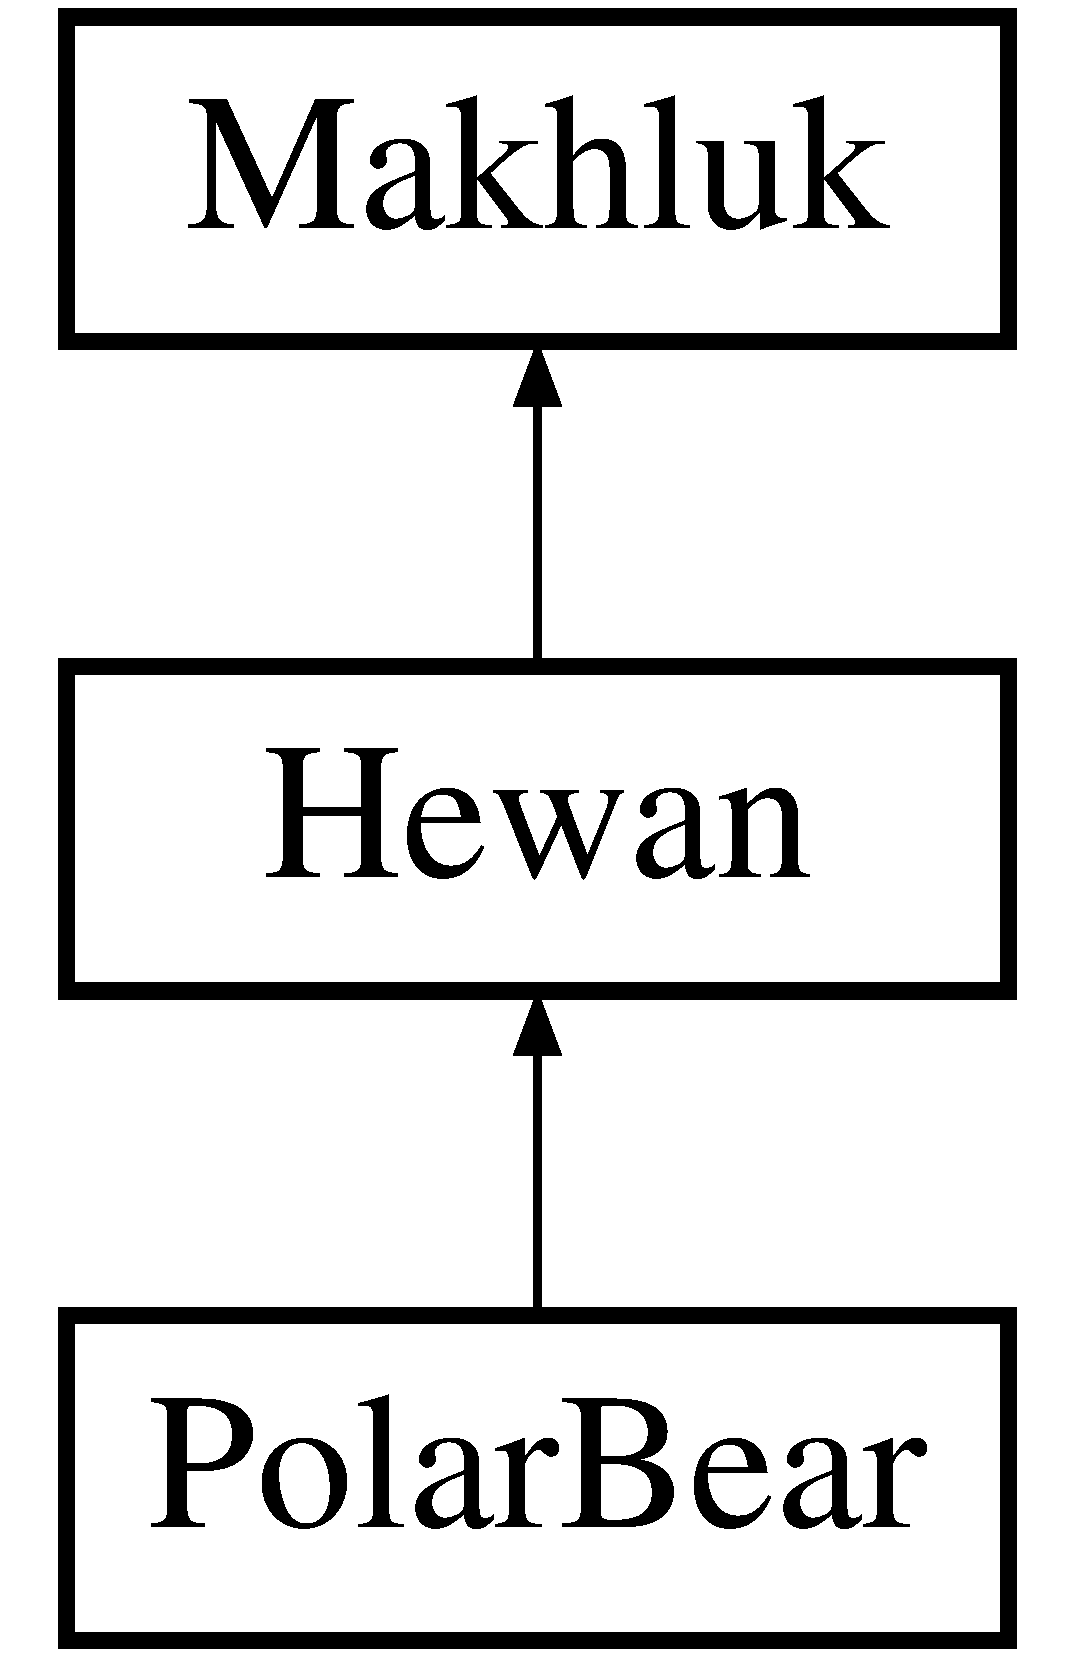
\includegraphics[height=3.000000cm]{class_polar_bear}
\end{center}
\end{figure}
\subsection*{Public Member Functions}
\begin{DoxyCompactItemize}
\item 
\hyperlink{class_polar_bear_ad6a4789bb79ea33f3f97e9e5e1b05810}{Polar\+Bear} (const \hyperlink{class_point}{Point} \&)
\begin{DoxyCompactList}\small\item\em Constructor. \end{DoxyCompactList}\item 
int \hyperlink{class_polar_bear_a528b34c3db1dee2cd5c06f6b6d221a14}{is\+Vegetarian} ()
\begin{DoxyCompactList}\small\item\em Fungsi untuk menentukan apakah \hyperlink{class_polar_bear}{Polar\+Bear} vegetarian. \end{DoxyCompactList}\item 
int \hyperlink{class_polar_bear_a636383dd8f5c357f205642a8b0354a55}{get\+DeltaT} ()
\begin{DoxyCompactList}\small\item\em Getter DeltaT \hyperlink{class_polar_bear}{Polar\+Bear}. \end{DoxyCompactList}\item 
void \hyperlink{class_polar_bear_a4b2f0d6aab60ceba83a1ced4c305ed3f}{Get\+To\+Food} ()
\begin{DoxyCompactList}\small\item\em Prosedur aksi \hyperlink{class_polar_bear}{Polar\+Bear} untuk mendapatkan makanan. \end{DoxyCompactList}\item 
void \hyperlink{class_polar_bear_aecb4f132a925275d4e730b58fc79158b}{Live} ()
\begin{DoxyCompactList}\small\item\em Prosedur hidup \hyperlink{class_polar_bear}{Polar\+Bear}. \end{DoxyCompactList}\end{DoxyCompactItemize}
\subsection*{Additional Inherited Members}


\subsection{Detailed Description}
Kelas turunan dari makhluk berupa \hyperlink{class_polar_bear}{Polar\+Bear}. 

Kelas \hyperlink{class_polar_bear}{Polar\+Bear} merupakan kelas yang berfungsi untuk mengatur behaviour dan kehidupan dari objek \hyperlink{class_polar_bear}{Polar\+Bear} \begin{DoxyAuthor}{Author}
Micky Yudi Utama 
\end{DoxyAuthor}
\begin{DoxyDate}{Date}
Maret 2016 
\end{DoxyDate}


\subsection{Constructor \& Destructor Documentation}
\index{Polar\+Bear@{Polar\+Bear}!Polar\+Bear@{Polar\+Bear}}
\index{Polar\+Bear@{Polar\+Bear}!Polar\+Bear@{Polar\+Bear}}
\subsubsection[{\texorpdfstring{Polar\+Bear(const Point \&)}{PolarBear(const Point &)}}]{\setlength{\rightskip}{0pt plus 5cm}Polar\+Bear\+::\+Polar\+Bear (
\begin{DoxyParamCaption}
\item[{const {\bf Point} \&}]{P}
\end{DoxyParamCaption}
)}\hypertarget{class_polar_bear_ad6a4789bb79ea33f3f97e9e5e1b05810}{}\label{class_polar_bear_ad6a4789bb79ea33f3f97e9e5e1b05810}


Constructor. 

Menciptakan objek \hyperlink{class_polar_bear}{Polar\+Bear} dengan posisi P 
\begin{DoxyParams}{Parameters}
{\em P} & const \hyperlink{class_point}{Point}\& Posisi objek \hyperlink{class_polar_bear}{Polar\+Bear} \\
\hline
\end{DoxyParams}


\subsection{Member Function Documentation}
\index{Polar\+Bear@{Polar\+Bear}!get\+DeltaT@{get\+DeltaT}}
\index{get\+DeltaT@{get\+DeltaT}!Polar\+Bear@{Polar\+Bear}}
\subsubsection[{\texorpdfstring{get\+Delta\+T()}{getDeltaT()}}]{\setlength{\rightskip}{0pt plus 5cm}int Polar\+Bear\+::get\+DeltaT (
\begin{DoxyParamCaption}
{}
\end{DoxyParamCaption}
)\hspace{0.3cm}{\ttfamily [inline]}}\hypertarget{class_polar_bear_a636383dd8f5c357f205642a8b0354a55}{}\label{class_polar_bear_a636383dd8f5c357f205642a8b0354a55}


Getter DeltaT \hyperlink{class_polar_bear}{Polar\+Bear}. 

Fungsi untuk memperoleh DeltaT makhluk \hyperlink{class_polar_bear}{Polar\+Bear} \begin{DoxyReturn}{Returns}
Bilangan bulat berupa DeltaT \hyperlink{class_polar_bear}{Polar\+Bear} 
\end{DoxyReturn}
\index{Polar\+Bear@{Polar\+Bear}!Get\+To\+Food@{Get\+To\+Food}}
\index{Get\+To\+Food@{Get\+To\+Food}!Polar\+Bear@{Polar\+Bear}}
\subsubsection[{\texorpdfstring{Get\+To\+Food()}{GetToFood()}}]{\setlength{\rightskip}{0pt plus 5cm}void Polar\+Bear\+::\+Get\+To\+Food (
\begin{DoxyParamCaption}
{}
\end{DoxyParamCaption}
)\hspace{0.3cm}{\ttfamily [virtual]}}\hypertarget{class_polar_bear_a4b2f0d6aab60ceba83a1ced4c305ed3f}{}\label{class_polar_bear_a4b2f0d6aab60ceba83a1ced4c305ed3f}


Prosedur aksi \hyperlink{class_polar_bear}{Polar\+Bear} untuk mendapatkan makanan. 

Prosedur aksi \hyperlink{class_polar_bear}{Polar\+Bear} untuk pergi ke makanannya \begin{DoxyReturn}{Returns}
void 
\end{DoxyReturn}


Implements \hyperlink{class_hewan_ab0478d48070dc3c51cda481f678ae40a}{Hewan}.

\index{Polar\+Bear@{Polar\+Bear}!is\+Vegetarian@{is\+Vegetarian}}
\index{is\+Vegetarian@{is\+Vegetarian}!Polar\+Bear@{Polar\+Bear}}
\subsubsection[{\texorpdfstring{is\+Vegetarian()}{isVegetarian()}}]{\setlength{\rightskip}{0pt plus 5cm}int Polar\+Bear\+::is\+Vegetarian (
\begin{DoxyParamCaption}
{}
\end{DoxyParamCaption}
)\hspace{0.3cm}{\ttfamily [inline]}, {\ttfamily [virtual]}}\hypertarget{class_polar_bear_a528b34c3db1dee2cd5c06f6b6d221a14}{}\label{class_polar_bear_a528b34c3db1dee2cd5c06f6b6d221a14}


Fungsi untuk menentukan apakah \hyperlink{class_polar_bear}{Polar\+Bear} vegetarian. 

Fungsi akan selalu mengembalikan bilangan bulat 0 karena \hyperlink{class_polar_bear}{Polar\+Bear} bukan vegetarian \begin{DoxyReturn}{Returns}
Bilangan bulat 0 
\end{DoxyReturn}


Implements \hyperlink{class_hewan_a90a316426af1d53add7ebf2a23ea9af2}{Hewan}.

\index{Polar\+Bear@{Polar\+Bear}!Live@{Live}}
\index{Live@{Live}!Polar\+Bear@{Polar\+Bear}}
\subsubsection[{\texorpdfstring{Live()}{Live()}}]{\setlength{\rightskip}{0pt plus 5cm}void Polar\+Bear\+::\+Live (
\begin{DoxyParamCaption}
{}
\end{DoxyParamCaption}
)\hspace{0.3cm}{\ttfamily [virtual]}}\hypertarget{class_polar_bear_aecb4f132a925275d4e730b58fc79158b}{}\label{class_polar_bear_aecb4f132a925275d4e730b58fc79158b}


Prosedur hidup \hyperlink{class_polar_bear}{Polar\+Bear}. 

Prosedur untuk menentukan apa yang akan dilakukan oleh \hyperlink{class_polar_bear}{Polar\+Bear} ketika masih hidup \begin{DoxyReturn}{Returns}
void 
\end{DoxyReturn}


Implements \hyperlink{class_makhluk}{Makhluk}.



The documentation for this class was generated from the following files\+:\begin{DoxyCompactItemize}
\item 
C\+:/\+Users/\+Ngiong/\+Documents/\+Git\+Hub/\+Tubes\+Makhluk/header/Polar\+Bear.\+h\item 
C\+:/\+Users/\+Ngiong/\+Documents/\+Git\+Hub/\+Tubes\+Makhluk/implementation/Polar\+Bear.\+cpp\end{DoxyCompactItemize}

\hypertarget{class_rabbit}{}\section{Rabbit Class Reference}
\label{class_rabbit}\index{Rabbit@{Rabbit}}


Kelas Turunan dari \hyperlink{class_makhluk}{Makhluk} berupa \hyperlink{class_rabbit}{Rabbit}.  




{\ttfamily \#include $<$Rabbit.\+h$>$}

Inheritance diagram for Rabbit\+:\begin{figure}[H]
\begin{center}
\leavevmode
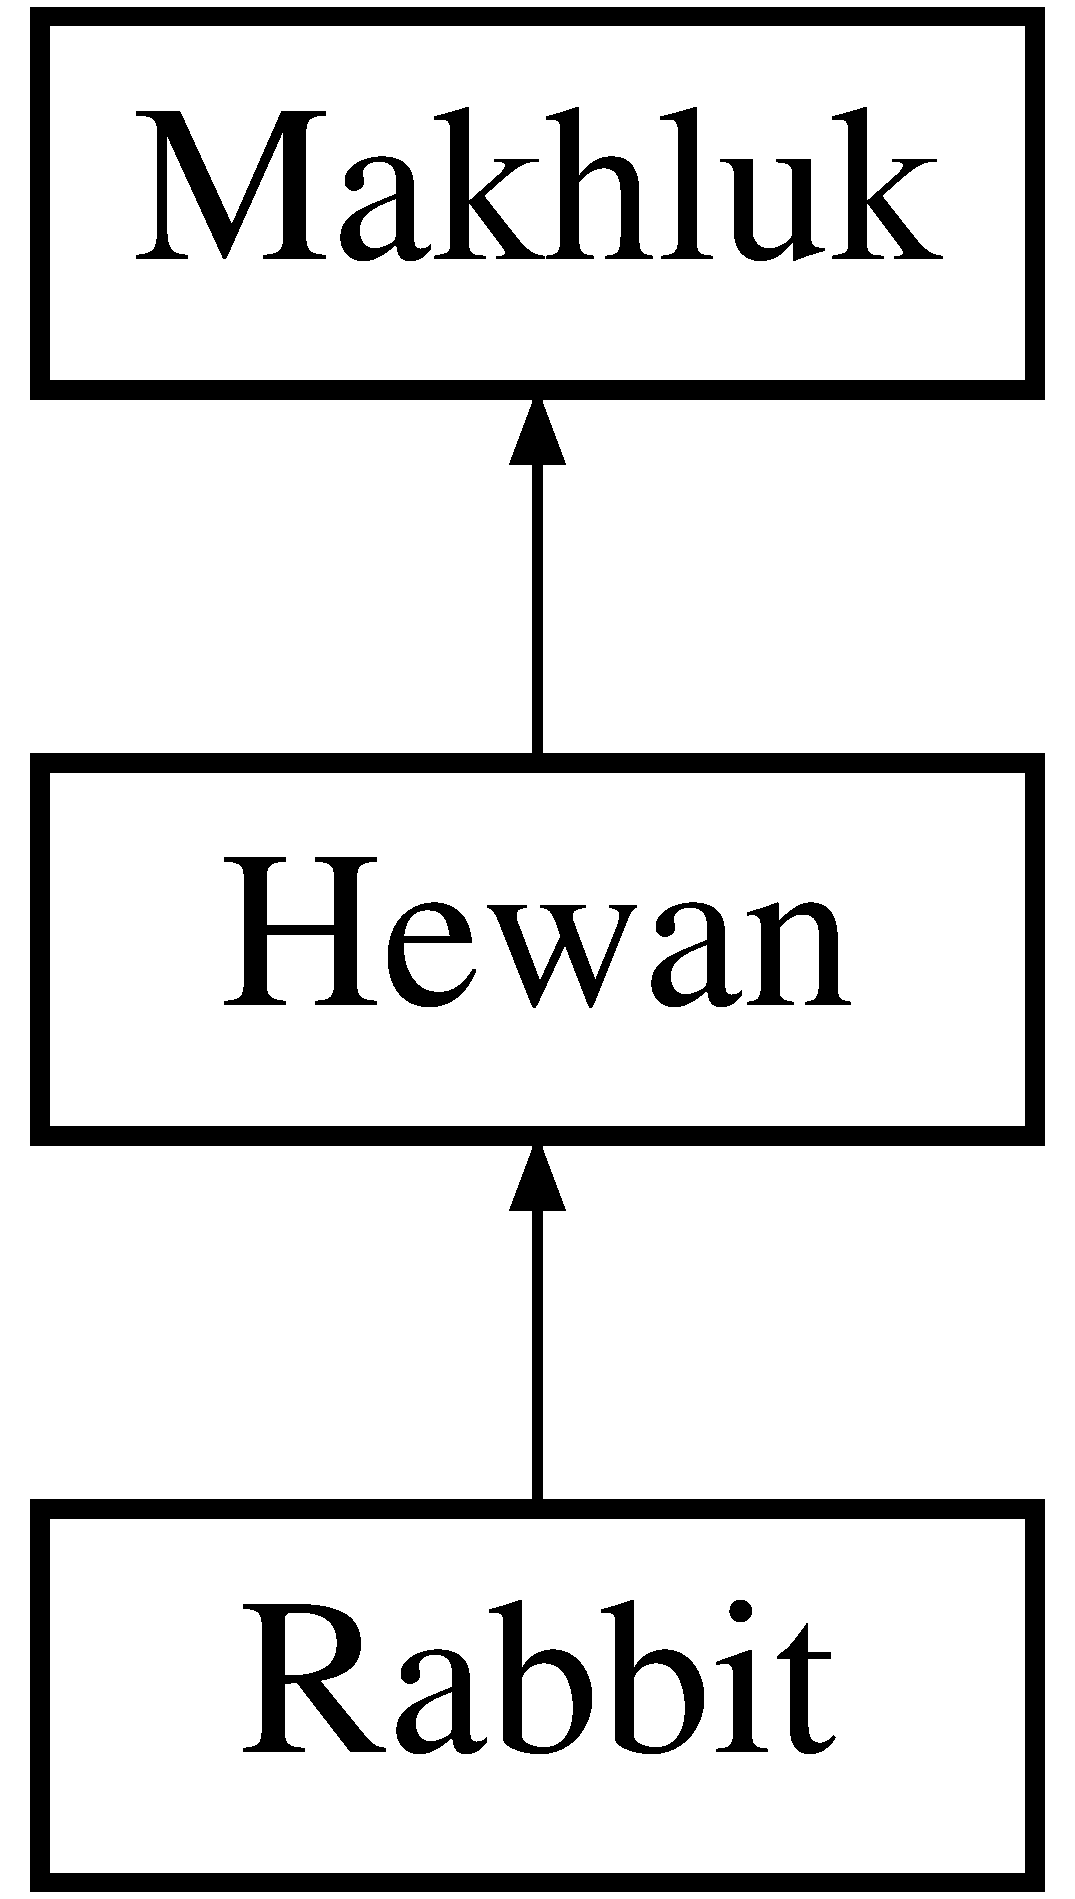
\includegraphics[height=3.000000cm]{class_rabbit}
\end{center}
\end{figure}
\subsection*{Public Member Functions}
\begin{DoxyCompactItemize}
\item 
\hyperlink{class_rabbit_ae7852b68a9ea0d4604a26a4a230dc44b}{Rabbit} (const \hyperlink{class_point}{Point} \&)
\begin{DoxyCompactList}\small\item\em Constructor dari objek bertipe \hyperlink{class_rabbit}{Rabbit}. \end{DoxyCompactList}\item 
int \hyperlink{class_rabbit_a58a0710c593b7bb19b7634d0ec1ad2ab}{is\+Vegetarian} ()
\begin{DoxyCompactList}\small\item\em Validasi apakah \hyperlink{class_rabbit}{Rabbit} merupakan Vegetarian. \end{DoxyCompactList}\item 
int \hyperlink{class_rabbit_ab0f37919999e5d906180426800210f67}{get\+DeltaT} ()
\begin{DoxyCompactList}\small\item\em Getter DeltaT \hyperlink{class_rabbit}{Rabbit}. \end{DoxyCompactList}\item 
void \hyperlink{class_rabbit_a94083faa62033470efbd9dd89afdb5a3}{Race} ()
\begin{DoxyCompactList}\small\item\em Procedure aksi untuk \hyperlink{class_rabbit}{Rabbit} melakukan Race dengan objek \hyperlink{class_turtle}{Turtle}. \end{DoxyCompactList}\item 
void \hyperlink{class_rabbit_a98d779a15b5b5b03fb15e62c06d01693}{Get\+To\+Food} ()
\begin{DoxyCompactList}\small\item\em Procedure aksi untuk \hyperlink{class_rabbit}{Rabbit} mendapatkan makanan. \end{DoxyCompactList}\item 
void \hyperlink{class_rabbit_ab9d8cfbbcf7b3e77e5e8996f2a2c662f}{Wandering\+Hop} ()
\begin{DoxyCompactList}\small\item\em Procedure aksi untuk \hyperlink{class_rabbit}{Rabbit} untuk berjalan di \hyperlink{class_world}{World} secara random dengan meloncat. \end{DoxyCompactList}\item 
void \hyperlink{class_rabbit_a6152392444f1d705cf6c0b1be36dca7a}{Live} ()
\begin{DoxyCompactList}\small\item\em Procedure aksi utama yang mengatur hidup \hyperlink{class_rabbit}{Rabbit} sampai mati. \end{DoxyCompactList}\end{DoxyCompactItemize}
\subsection*{Additional Inherited Members}


\subsection{Detailed Description}
Kelas Turunan dari \hyperlink{class_makhluk}{Makhluk} berupa \hyperlink{class_rabbit}{Rabbit}. 

Kelas \hyperlink{class_rabbit}{Rabbit} merupakan kelas yang berfungsi untuk mengatur behaviour dan kehidupan dari objek \hyperlink{class_rabbit}{Rabbit} \begin{DoxyAuthor}{Author}
Atika Azzahra Akbar 
\end{DoxyAuthor}
\begin{DoxyDate}{Date}
Maret 2016 
\end{DoxyDate}


\subsection{Constructor \& Destructor Documentation}
\index{Rabbit@{Rabbit}!Rabbit@{Rabbit}}
\index{Rabbit@{Rabbit}!Rabbit@{Rabbit}}
\subsubsection[{\texorpdfstring{Rabbit(const Point \&)}{Rabbit(const Point &)}}]{\setlength{\rightskip}{0pt plus 5cm}Rabbit\+::\+Rabbit (
\begin{DoxyParamCaption}
\item[{const {\bf Point} \&}]{P}
\end{DoxyParamCaption}
)}\hypertarget{class_rabbit_ae7852b68a9ea0d4604a26a4a230dc44b}{}\label{class_rabbit_ae7852b68a9ea0d4604a26a4a230dc44b}


Constructor dari objek bertipe \hyperlink{class_rabbit}{Rabbit}. 

Constructor \hyperlink{class_rabbit}{Rabbit} yang akan membentuk objek bertipe \hyperlink{class_rabbit}{Rabbit} dengan masukan variable reference \hyperlink{class_point}{Point} sebagai posisi awal objek \begin{DoxyReturn}{Returns}
Objek bertipe \hyperlink{class_rabbit}{Rabbit} 
\end{DoxyReturn}


\subsection{Member Function Documentation}
\index{Rabbit@{Rabbit}!get\+DeltaT@{get\+DeltaT}}
\index{get\+DeltaT@{get\+DeltaT}!Rabbit@{Rabbit}}
\subsubsection[{\texorpdfstring{get\+Delta\+T()}{getDeltaT()}}]{\setlength{\rightskip}{0pt plus 5cm}int Rabbit\+::get\+DeltaT (
\begin{DoxyParamCaption}
{}
\end{DoxyParamCaption}
)\hspace{0.3cm}{\ttfamily [inline]}}\hypertarget{class_rabbit_ab0f37919999e5d906180426800210f67}{}\label{class_rabbit_ab0f37919999e5d906180426800210f67}


Getter DeltaT \hyperlink{class_rabbit}{Rabbit}. 

Fungsi getter yang akan mengambilkan nilai deltaT dari \hyperlink{class_rabbit}{Rabbit} yang merupakan member dari kelas hewan yang diinisialisasi saat ctor \begin{DoxyReturn}{Returns}
Integer DeltaT \hyperlink{class_rabbit}{Rabbit} 
\end{DoxyReturn}
\index{Rabbit@{Rabbit}!Get\+To\+Food@{Get\+To\+Food}}
\index{Get\+To\+Food@{Get\+To\+Food}!Rabbit@{Rabbit}}
\subsubsection[{\texorpdfstring{Get\+To\+Food()}{GetToFood()}}]{\setlength{\rightskip}{0pt plus 5cm}void Rabbit\+::\+Get\+To\+Food (
\begin{DoxyParamCaption}
{}
\end{DoxyParamCaption}
)\hspace{0.3cm}{\ttfamily [virtual]}}\hypertarget{class_rabbit_a98d779a15b5b5b03fb15e62c06d01693}{}\label{class_rabbit_a98d779a15b5b5b03fb15e62c06d01693}


Procedure aksi untuk \hyperlink{class_rabbit}{Rabbit} mendapatkan makanan. 

Procedure aksi Get\+To\+Food membuat \hyperlink{class_rabbit}{Rabbit} pergi ke point dimana makanannya berasa dan memakannya \begin{DoxyReturn}{Returns}
void 
\end{DoxyReturn}


Implements \hyperlink{class_hewan_ab0478d48070dc3c51cda481f678ae40a}{Hewan}.

\index{Rabbit@{Rabbit}!is\+Vegetarian@{is\+Vegetarian}}
\index{is\+Vegetarian@{is\+Vegetarian}!Rabbit@{Rabbit}}
\subsubsection[{\texorpdfstring{is\+Vegetarian()}{isVegetarian()}}]{\setlength{\rightskip}{0pt plus 5cm}int Rabbit\+::is\+Vegetarian (
\begin{DoxyParamCaption}
{}
\end{DoxyParamCaption}
)\hspace{0.3cm}{\ttfamily [inline]}, {\ttfamily [virtual]}}\hypertarget{class_rabbit_a58a0710c593b7bb19b7634d0ec1ad2ab}{}\label{class_rabbit_a58a0710c593b7bb19b7634d0ec1ad2ab}


Validasi apakah \hyperlink{class_rabbit}{Rabbit} merupakan Vegetarian. 

Validasi akan selalu mengembalikan integer bernilai 1 sebagai validasi bahwa \hyperlink{class_rabbit}{Rabbit} merupakan binatang vegetarian \begin{DoxyReturn}{Returns}
integer bernilai 1 
\end{DoxyReturn}


Implements \hyperlink{class_hewan_a90a316426af1d53add7ebf2a23ea9af2}{Hewan}.

\index{Rabbit@{Rabbit}!Live@{Live}}
\index{Live@{Live}!Rabbit@{Rabbit}}
\subsubsection[{\texorpdfstring{Live()}{Live()}}]{\setlength{\rightskip}{0pt plus 5cm}void Rabbit\+::\+Live (
\begin{DoxyParamCaption}
{}
\end{DoxyParamCaption}
)\hspace{0.3cm}{\ttfamily [virtual]}}\hypertarget{class_rabbit_a6152392444f1d705cf6c0b1be36dca7a}{}\label{class_rabbit_a6152392444f1d705cf6c0b1be36dca7a}


Procedure aksi utama yang mengatur hidup \hyperlink{class_rabbit}{Rabbit} sampai mati. 

Procedure aksi utama akan memilih aktivitas kehidupan yang akan dilakukan oleh \hyperlink{class_rabbit}{Rabbit} selama hidupnya \begin{DoxyReturn}{Returns}
void 
\end{DoxyReturn}


Implements \hyperlink{class_makhluk}{Makhluk}.

\index{Rabbit@{Rabbit}!Race@{Race}}
\index{Race@{Race}!Rabbit@{Rabbit}}
\subsubsection[{\texorpdfstring{Race()}{Race()}}]{\setlength{\rightskip}{0pt plus 5cm}void Rabbit\+::\+Race (
\begin{DoxyParamCaption}
{}
\end{DoxyParamCaption}
)}\hypertarget{class_rabbit_a94083faa62033470efbd9dd89afdb5a3}{}\label{class_rabbit_a94083faa62033470efbd9dd89afdb5a3}


Procedure aksi untuk \hyperlink{class_rabbit}{Rabbit} melakukan Race dengan objek \hyperlink{class_turtle}{Turtle}. 

Procedure aksi Race ini akan memberikan ajakan race untuk objek \hyperlink{class_turtle}{Turtle}, pergi ke point start, dan melakukan race bersama \hyperlink{class_turtle}{Turtle} ke finish point \begin{DoxyReturn}{Returns}
void 
\end{DoxyReturn}
\index{Rabbit@{Rabbit}!Wandering\+Hop@{Wandering\+Hop}}
\index{Wandering\+Hop@{Wandering\+Hop}!Rabbit@{Rabbit}}
\subsubsection[{\texorpdfstring{Wandering\+Hop()}{WanderingHop()}}]{\setlength{\rightskip}{0pt plus 5cm}void Rabbit\+::\+Wandering\+Hop (
\begin{DoxyParamCaption}
{}
\end{DoxyParamCaption}
)}\hypertarget{class_rabbit_ab9d8cfbbcf7b3e77e5e8996f2a2c662f}{}\label{class_rabbit_ab9d8cfbbcf7b3e77e5e8996f2a2c662f}


Procedure aksi untuk \hyperlink{class_rabbit}{Rabbit} untuk berjalan di \hyperlink{class_world}{World} secara random dengan meloncat. 

Procedure aksi ini merupakan procedure implementasi behaviour khusus \hyperlink{class_rabbit}{Rabbit} dimana \hyperlink{class_rabbit}{Rabbit} meloncati dua sel sekali berjalan secara random di \hyperlink{class_world}{World} \begin{DoxyReturn}{Returns}
void 
\end{DoxyReturn}


The documentation for this class was generated from the following files\+:\begin{DoxyCompactItemize}
\item 
C\+:/\+Users/\+Ngiong/\+Documents/\+Git\+Hub/\+Tubes\+Makhluk/header/Rabbit.\+h\item 
C\+:/\+Users/\+Ngiong/\+Documents/\+Git\+Hub/\+Tubes\+Makhluk/implementation/Rabbit.\+cpp\end{DoxyCompactItemize}

\hypertarget{class_random_generator}{}\section{Random\+Generator Class Reference}
\label{class_random_generator}\index{Random\+Generator@{Random\+Generator}}


Mengembalikan random number.  




{\ttfamily \#include $<$Random\+Generator.\+h$>$}

\subsection*{Public Member Functions}
\begin{DoxyCompactItemize}
\item 
int \hyperlink{class_random_generator_a7bdfd5b421ffaa1de622804fee51c3eb}{get\+Next\+Int} (int)
\begin{DoxyCompactList}\small\item\em Fungsi untuk mengacak bilangan bulat berdasarkan batasan. \end{DoxyCompactList}\item 
int \hyperlink{class_random_generator_ab230d076577cb8a5719b866ad2d23460}{get\+Next\+Int\+Between} (int, int)
\begin{DoxyCompactList}\small\item\em Fungsi untuk mengacak bilangan bulat berdasarkan batasan. \end{DoxyCompactList}\item 
\hyperlink{class_point}{Point} \hyperlink{class_random_generator_a4c6407b76023eed6f10e58996c0fdcae}{get\+Next\+Point} (int, int)
\begin{DoxyCompactList}\small\item\em Fungsi untuk mengacak point berdasarkan batasan. \end{DoxyCompactList}\item 
\hyperlink{class_point}{Point} \hyperlink{class_random_generator_a69f7d43d8f1ce21306612eb939e4f347}{get\+Next\+Point\+PB} (int, int)
\begin{DoxyCompactList}\small\item\em Fungsi untuk mengacak point berdasarkan batasan. \end{DoxyCompactList}\item 
void \hyperlink{class_random_generator_a8e8c1e6e1f4cc57c2bd463cf26903110}{lock\+Random} ()
\begin{DoxyCompactList}\small\item\em Mutex. \end{DoxyCompactList}\item 
void \hyperlink{class_random_generator_affa68e83ee3598b50cf9de4fd093fe6a}{unlock\+Random} ()
\begin{DoxyCompactList}\small\item\em Mutex. \end{DoxyCompactList}\end{DoxyCompactItemize}
\subsection*{Static Public Member Functions}
\begin{DoxyCompactItemize}
\item 
static \hyperlink{class_random_generator}{Random\+Generator} $\ast$ \hyperlink{class_random_generator_abc2ce3ecccf8a36af2ab362effd7e5a1}{get\+Instance} ()
\begin{DoxyCompactList}\small\item\em Get singleton instance dari kelas \hyperlink{class_random_generator}{Random\+Generator}. \end{DoxyCompactList}\end{DoxyCompactItemize}


\subsection{Detailed Description}
Mengembalikan random number. 

Kelas \hyperlink{class_random_generator}{Random\+Generator} mengembalikan sebuah random number berdasarkan batasan yang diberikan \begin{DoxyAuthor}{Author}
Micky Yudi Utama 
\end{DoxyAuthor}
\begin{DoxyDate}{Date}
Maret 2016 
\end{DoxyDate}


\subsection{Member Function Documentation}
\index{Random\+Generator@{Random\+Generator}!get\+Instance@{get\+Instance}}
\index{get\+Instance@{get\+Instance}!Random\+Generator@{Random\+Generator}}
\subsubsection[{\texorpdfstring{get\+Instance()}{getInstance()}}]{\setlength{\rightskip}{0pt plus 5cm}static {\bf Random\+Generator}$\ast$ Random\+Generator\+::get\+Instance (
\begin{DoxyParamCaption}
{}
\end{DoxyParamCaption}
)\hspace{0.3cm}{\ttfamily [inline]}, {\ttfamily [static]}}\hypertarget{class_random_generator_abc2ce3ecccf8a36af2ab362effd7e5a1}{}\label{class_random_generator_abc2ce3ecccf8a36af2ab362effd7e5a1}


Get singleton instance dari kelas \hyperlink{class_random_generator}{Random\+Generator}. 

Mengembalikan pointer dari objek kelas singleton pada kelas \hyperlink{class_random_generator}{Random\+Generator} \begin{DoxyReturn}{Returns}
Pointer yang menunjuk ke singleton instance pada kelas \hyperlink{class_random_generator}{Random\+Generator} 
\end{DoxyReturn}
\index{Random\+Generator@{Random\+Generator}!get\+Next\+Int@{get\+Next\+Int}}
\index{get\+Next\+Int@{get\+Next\+Int}!Random\+Generator@{Random\+Generator}}
\subsubsection[{\texorpdfstring{get\+Next\+Int(int)}{getNextInt(int)}}]{\setlength{\rightskip}{0pt plus 5cm}int Random\+Generator\+::get\+Next\+Int (
\begin{DoxyParamCaption}
\item[{int}]{a}
\end{DoxyParamCaption}
)}\hypertarget{class_random_generator_a7bdfd5b421ffaa1de622804fee51c3eb}{}\label{class_random_generator_a7bdfd5b421ffaa1de622804fee51c3eb}


Fungsi untuk mengacak bilangan bulat berdasarkan batasan. 

Melakukan pengacakan bilangan bulat dengan batasan (0...a-\/1) 
\begin{DoxyParams}{Parameters}
{\em a} & int Batas atas hasil acak \\
\hline
\end{DoxyParams}
\begin{DoxyReturn}{Returns}
Bilangan bulat acak dari (0...a-\/1) 
\end{DoxyReturn}
\index{Random\+Generator@{Random\+Generator}!get\+Next\+Int\+Between@{get\+Next\+Int\+Between}}
\index{get\+Next\+Int\+Between@{get\+Next\+Int\+Between}!Random\+Generator@{Random\+Generator}}
\subsubsection[{\texorpdfstring{get\+Next\+Int\+Between(int, int)}{getNextIntBetween(int, int)}}]{\setlength{\rightskip}{0pt plus 5cm}int Random\+Generator\+::get\+Next\+Int\+Between (
\begin{DoxyParamCaption}
\item[{int}]{a, }
\item[{int}]{b}
\end{DoxyParamCaption}
)}\hypertarget{class_random_generator_ab230d076577cb8a5719b866ad2d23460}{}\label{class_random_generator_ab230d076577cb8a5719b866ad2d23460}


Fungsi untuk mengacak bilangan bulat berdasarkan batasan. 

Melakukan pengacakan bilangan bulat dengan batasan (a...b) 
\begin{DoxyParams}{Parameters}
{\em a} & int Batas bawah hasil acak \\
\hline
{\em b} & int Batas atas hasil acak \\
\hline
\end{DoxyParams}
\begin{DoxyReturn}{Returns}
Bilangan bulat acak dari (a...b) 
\end{DoxyReturn}
\index{Random\+Generator@{Random\+Generator}!get\+Next\+Point@{get\+Next\+Point}}
\index{get\+Next\+Point@{get\+Next\+Point}!Random\+Generator@{Random\+Generator}}
\subsubsection[{\texorpdfstring{get\+Next\+Point(int, int)}{getNextPoint(int, int)}}]{\setlength{\rightskip}{0pt plus 5cm}{\bf Point} Random\+Generator\+::get\+Next\+Point (
\begin{DoxyParamCaption}
\item[{int}]{N\+Brs, }
\item[{int}]{N\+Kol}
\end{DoxyParamCaption}
)}\hypertarget{class_random_generator_a4c6407b76023eed6f10e58996c0fdcae}{}\label{class_random_generator_a4c6407b76023eed6f10e58996c0fdcae}


Fungsi untuk mengacak point berdasarkan batasan. 

Melakukan pengacakan point dengan batasan (1...Nbrs-\/2), (1...N\+Kol-\/2) 
\begin{DoxyParams}{Parameters}
{\em N\+Brs} & int Jumlah baris \\
\hline
{\em N\+Kol} & int Jumlah kolom \\
\hline
\end{DoxyParams}
\begin{DoxyReturn}{Returns}
\hyperlink{class_point}{Point} acak dari (1...Nbrs-\/2), (1...N\+Kol-\/2) 
\end{DoxyReturn}
\index{Random\+Generator@{Random\+Generator}!get\+Next\+Point\+PB@{get\+Next\+Point\+PB}}
\index{get\+Next\+Point\+PB@{get\+Next\+Point\+PB}!Random\+Generator@{Random\+Generator}}
\subsubsection[{\texorpdfstring{get\+Next\+Point\+P\+B(int, int)}{getNextPointPB(int, int)}}]{\setlength{\rightskip}{0pt plus 5cm}{\bf Point} Random\+Generator\+::get\+Next\+Point\+PB (
\begin{DoxyParamCaption}
\item[{int}]{N\+Brs, }
\item[{int}]{N\+Kol}
\end{DoxyParamCaption}
)}\hypertarget{class_random_generator_a69f7d43d8f1ce21306612eb939e4f347}{}\label{class_random_generator_a69f7d43d8f1ce21306612eb939e4f347}


Fungsi untuk mengacak point berdasarkan batasan. 

Melakukan pengacakan point dengan batasan (N\+Brs-\/(N\+Brs/5)-\/2...Nbrs-\/2), (1...N\+Kol-\/2) 
\begin{DoxyParams}{Parameters}
{\em N\+Brs} & int Jumlah baris \\
\hline
{\em N\+Kol} & int Jumlah kolom \\
\hline
\end{DoxyParams}
\begin{DoxyReturn}{Returns}
\hyperlink{class_point}{Point} acak dari (N\+Brs-\/(N\+Brs/5)-\/2...Nbrs-\/2), (1...N\+Kol-\/2) 
\end{DoxyReturn}
\index{Random\+Generator@{Random\+Generator}!lock\+Random@{lock\+Random}}
\index{lock\+Random@{lock\+Random}!Random\+Generator@{Random\+Generator}}
\subsubsection[{\texorpdfstring{lock\+Random()}{lockRandom()}}]{\setlength{\rightskip}{0pt plus 5cm}void Random\+Generator\+::lock\+Random (
\begin{DoxyParamCaption}
{}
\end{DoxyParamCaption}
)}\hypertarget{class_random_generator_a8e8c1e6e1f4cc57c2bd463cf26903110}{}\label{class_random_generator_a8e8c1e6e1f4cc57c2bd463cf26903110}


Mutex. 

Mengunci akses untuk menggunakan random \begin{DoxyReturn}{Returns}
void 
\end{DoxyReturn}
\index{Random\+Generator@{Random\+Generator}!unlock\+Random@{unlock\+Random}}
\index{unlock\+Random@{unlock\+Random}!Random\+Generator@{Random\+Generator}}
\subsubsection[{\texorpdfstring{unlock\+Random()}{unlockRandom()}}]{\setlength{\rightskip}{0pt plus 5cm}void Random\+Generator\+::unlock\+Random (
\begin{DoxyParamCaption}
{}
\end{DoxyParamCaption}
)}\hypertarget{class_random_generator_affa68e83ee3598b50cf9de4fd093fe6a}{}\label{class_random_generator_affa68e83ee3598b50cf9de4fd093fe6a}


Mutex. 

Membuka akses untuk menggunakan random \begin{DoxyReturn}{Returns}
void 
\end{DoxyReturn}


The documentation for this class was generated from the following files\+:\begin{DoxyCompactItemize}
\item 
C\+:/\+Users/\+Ngiong/\+Documents/\+Git\+Hub/\+Tubes\+Makhluk/v3/header/Random\+Generator.\+h\item 
C\+:/\+Users/\+Ngiong/\+Documents/\+Git\+Hub/\+Tubes\+Makhluk/v3/implementation/Random\+Generator.\+cpp\end{DoxyCompactItemize}

\hypertarget{class_screen}{}\section{Screen Class Reference}
\label{class_screen}\index{Screen@{Screen}}


Representasi dari layar pengguna.  




{\ttfamily \#include $<$Screen.\+h$>$}

\subsection*{Public Member Functions}
\begin{DoxyCompactItemize}
\item 
void \hyperlink{class_screen_aebdf6e729abb754cb4c6a2b65ff44d84}{Print\+Matrix} (const \hyperlink{class_matrix}{Matrix} \&)
\begin{DoxyCompactList}\small\item\em Mencetak sebuah matriks ke layar. \end{DoxyCompactList}\item 
void \hyperlink{class_screen_ae87ec3a6c85d019370bf5a73d38e4f7e}{Print\+World\+Map} ()
\begin{DoxyCompactList}\small\item\em Mencetak dunia beserta isinya. \end{DoxyCompactList}\end{DoxyCompactItemize}
\subsection*{Static Public Member Functions}
\begin{DoxyCompactItemize}
\item 
static \hyperlink{class_screen}{Screen} $\ast$ \hyperlink{class_screen_a6600999f98834ff40a2a42d291867db2}{get\+Screen\+Instance} ()
\begin{DoxyCompactList}\small\item\em Get Singleton Instance dari kelas \hyperlink{class_screen}{Screen}. \end{DoxyCompactList}\item 
static void \hyperlink{class_screen_a116d9815de49d2a74bc3c558e4322130}{Show\+World} (int)
\begin{DoxyCompactList}\small\item\em Mencetak dunia beserta isinya secara berkala. \end{DoxyCompactList}\end{DoxyCompactItemize}


\subsection{Detailed Description}
Representasi dari layar pengguna. 

Kelas \hyperlink{class_screen}{Screen} merepresentasikan layar pengguna dan bertanggung jawab untuk melakukan operasi-\/operasi Input-\/\+Output. \begin{DoxyAuthor}{Author}
Robert Sebastian Herlim 
\end{DoxyAuthor}
\begin{DoxyDate}{Date}
Maret 2016 
\end{DoxyDate}


\subsection{Member Function Documentation}
\index{Screen@{Screen}!get\+Screen\+Instance@{get\+Screen\+Instance}}
\index{get\+Screen\+Instance@{get\+Screen\+Instance}!Screen@{Screen}}
\subsubsection[{\texorpdfstring{get\+Screen\+Instance()}{getScreenInstance()}}]{\setlength{\rightskip}{0pt plus 5cm}static {\bf Screen}$\ast$ Screen\+::get\+Screen\+Instance (
\begin{DoxyParamCaption}
{}
\end{DoxyParamCaption}
)\hspace{0.3cm}{\ttfamily [inline]}, {\ttfamily [static]}}\hypertarget{class_screen_a6600999f98834ff40a2a42d291867db2}{}\label{class_screen_a6600999f98834ff40a2a42d291867db2}


Get Singleton Instance dari kelas \hyperlink{class_screen}{Screen}. 

Mengembalikan pointer dari objek singleton pada kelas \hyperlink{class_screen}{Screen} \begin{DoxyReturn}{Returns}
pointer yang menunjuk ke singleton instance pada kelas \hyperlink{class_screen}{Screen} 
\end{DoxyReturn}
\index{Screen@{Screen}!Print\+Matrix@{Print\+Matrix}}
\index{Print\+Matrix@{Print\+Matrix}!Screen@{Screen}}
\subsubsection[{\texorpdfstring{Print\+Matrix(const Matrix \&)}{PrintMatrix(const Matrix &)}}]{\setlength{\rightskip}{0pt plus 5cm}void Screen\+::\+Print\+Matrix (
\begin{DoxyParamCaption}
\item[{const {\bf Matrix} \&}]{M}
\end{DoxyParamCaption}
)}\hypertarget{class_screen_aebdf6e729abb754cb4c6a2b65ff44d84}{}\label{class_screen_aebdf6e729abb754cb4c6a2b65ff44d84}


Mencetak sebuah matriks ke layar. 

Mencetak sebuah matriks ke layar \begin{DoxyReturn}{Returns}
void 
\end{DoxyReturn}
\index{Screen@{Screen}!Print\+World\+Map@{Print\+World\+Map}}
\index{Print\+World\+Map@{Print\+World\+Map}!Screen@{Screen}}
\subsubsection[{\texorpdfstring{Print\+World\+Map()}{PrintWorldMap()}}]{\setlength{\rightskip}{0pt plus 5cm}void Screen\+::\+Print\+World\+Map (
\begin{DoxyParamCaption}
{}
\end{DoxyParamCaption}
)}\hypertarget{class_screen_ae87ec3a6c85d019370bf5a73d38e4f7e}{}\label{class_screen_ae87ec3a6c85d019370bf5a73d38e4f7e}


Mencetak dunia beserta isinya. 

Mencetak sebuah state dunia beserta pada waktu tertentu dengan makhluk-\/makhluk yang ada di dalamnya ke layar \begin{DoxyReturn}{Returns}
void 
\end{DoxyReturn}
\index{Screen@{Screen}!Show\+World@{Show\+World}}
\index{Show\+World@{Show\+World}!Screen@{Screen}}
\subsubsection[{\texorpdfstring{Show\+World(int)}{ShowWorld(int)}}]{\setlength{\rightskip}{0pt plus 5cm}void Screen\+::\+Show\+World (
\begin{DoxyParamCaption}
\item[{int}]{deltaT}
\end{DoxyParamCaption}
)\hspace{0.3cm}{\ttfamily [static]}}\hypertarget{class_screen_a116d9815de49d2a74bc3c558e4322130}{}\label{class_screen_a116d9815de49d2a74bc3c558e4322130}


Mencetak dunia beserta isinya secara berkala. 

Mencetak state dunia beserta dengan isi-\/isinya ke layar secara berkala dengan interval waktu tertentu 
\begin{DoxyParams}{Parameters}
{\em deltaT} & int interval waktu (dalam ms) antar pencetakan state dunia ke layar \\
\hline
\end{DoxyParams}
\begin{DoxyReturn}{Returns}
void 
\end{DoxyReturn}


The documentation for this class was generated from the following files\+:\begin{DoxyCompactItemize}
\item 
C\+:/\+Users/\+Ngiong/\+Documents/\+Git\+Hub/\+Tubes\+Makhluk/header/Screen.\+h\item 
C\+:/\+Users/\+Ngiong/\+Documents/\+Git\+Hub/\+Tubes\+Makhluk/implementation/Screen.\+cpp\end{DoxyCompactItemize}

\hypertarget{class_sheep}{}\section{Sheep Class Reference}
\label{class_sheep}\index{Sheep@{Sheep}}


Kelas turunan dari makhluk berupa \hyperlink{class_sheep}{Sheep}.  




{\ttfamily \#include $<$Sheep.\+h$>$}

Inheritance diagram for Sheep\+:\begin{figure}[H]
\begin{center}
\leavevmode
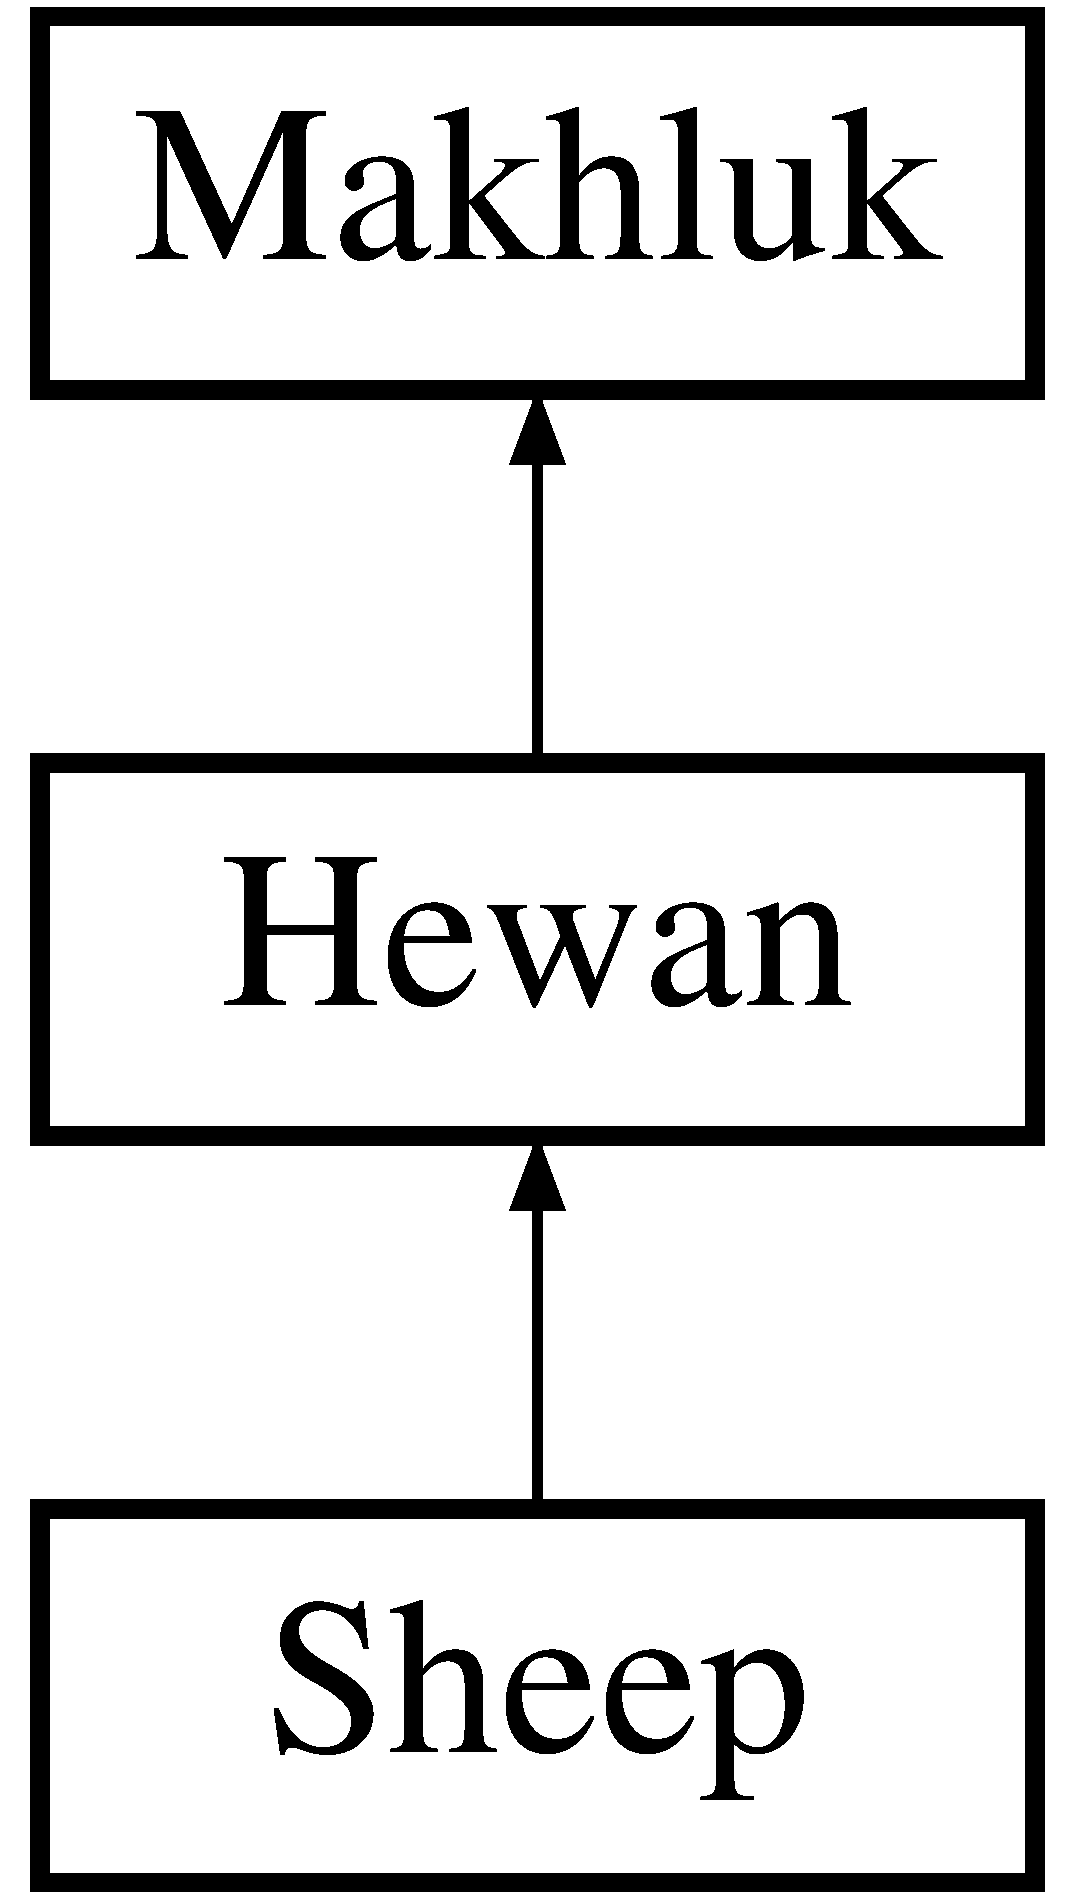
\includegraphics[height=3.000000cm]{class_sheep}
\end{center}
\end{figure}
\subsection*{Public Member Functions}
\begin{DoxyCompactItemize}
\item 
\hyperlink{class_sheep_a4b3c6eac247be02dfbc9628d594cd04d}{Sheep} (const \hyperlink{class_point}{Point} \&)
\begin{DoxyCompactList}\small\item\em Constructor. \end{DoxyCompactList}\item 
int \hyperlink{class_sheep_a5210b51ab73a9f562111405d6e0ecb46}{is\+Vegetarian} ()
\begin{DoxyCompactList}\small\item\em Fungsi untuk menentukan apakah \hyperlink{class_sheep}{Sheep} vegetarian. \end{DoxyCompactList}\item 
int \hyperlink{class_sheep_ab308d0c603fd3405d5acd5717497a47b}{get\+DeltaT} ()
\begin{DoxyCompactList}\small\item\em Getter DeltaT \hyperlink{class_wolf}{Wolf}. \end{DoxyCompactList}\item 
void \hyperlink{class_sheep_a134766a3fc3060b5a1dd39aa11df262d}{Get\+To\+Food} ()
\begin{DoxyCompactList}\small\item\em Prosedur aksi \hyperlink{class_sheep}{Sheep} untuk mendapatkan makanan. \end{DoxyCompactList}\item 
void \hyperlink{class_sheep_a3a808c6656a9d932f5ec4043c301727b}{Live} ()
\begin{DoxyCompactList}\small\item\em Prosedur hidup \hyperlink{class_sheep}{Sheep}. \end{DoxyCompactList}\end{DoxyCompactItemize}
\subsection*{Additional Inherited Members}


\subsection{Detailed Description}
Kelas turunan dari makhluk berupa \hyperlink{class_sheep}{Sheep}. 

Kelas \hyperlink{class_sheep}{Sheep} merupakan kelas yang berfungsi untuk mengatur behaviour dan kehidupan dari objek \hyperlink{class_sheep}{Sheep} \begin{DoxyAuthor}{Author}
Micky Yudi Utama 
\end{DoxyAuthor}
\begin{DoxyDate}{Date}
Maret 2016 
\end{DoxyDate}


\subsection{Constructor \& Destructor Documentation}
\index{Sheep@{Sheep}!Sheep@{Sheep}}
\index{Sheep@{Sheep}!Sheep@{Sheep}}
\subsubsection[{\texorpdfstring{Sheep(const Point \&)}{Sheep(const Point &)}}]{\setlength{\rightskip}{0pt plus 5cm}Sheep\+::\+Sheep (
\begin{DoxyParamCaption}
\item[{const {\bf Point} \&}]{P}
\end{DoxyParamCaption}
)}\hypertarget{class_sheep_a4b3c6eac247be02dfbc9628d594cd04d}{}\label{class_sheep_a4b3c6eac247be02dfbc9628d594cd04d}


Constructor. 

Menciptakan objek \hyperlink{class_sheep}{Sheep} dengan posisi P 
\begin{DoxyParams}{Parameters}
{\em P} & const \hyperlink{class_point}{Point}\& Posisi objek \hyperlink{class_wolf}{Wolf} \\
\hline
\end{DoxyParams}


\subsection{Member Function Documentation}
\index{Sheep@{Sheep}!get\+DeltaT@{get\+DeltaT}}
\index{get\+DeltaT@{get\+DeltaT}!Sheep@{Sheep}}
\subsubsection[{\texorpdfstring{get\+Delta\+T()}{getDeltaT()}}]{\setlength{\rightskip}{0pt plus 5cm}int Sheep\+::get\+DeltaT (
\begin{DoxyParamCaption}
{}
\end{DoxyParamCaption}
)\hspace{0.3cm}{\ttfamily [inline]}}\hypertarget{class_sheep_ab308d0c603fd3405d5acd5717497a47b}{}\label{class_sheep_ab308d0c603fd3405d5acd5717497a47b}


Getter DeltaT \hyperlink{class_wolf}{Wolf}. 

Fungsi untuk memperoleh DeltaT makhluk \hyperlink{class_wolf}{Wolf} \begin{DoxyReturn}{Returns}
Bilangan bulat berupa DeltaT \hyperlink{class_wolf}{Wolf} 
\end{DoxyReturn}
\index{Sheep@{Sheep}!Get\+To\+Food@{Get\+To\+Food}}
\index{Get\+To\+Food@{Get\+To\+Food}!Sheep@{Sheep}}
\subsubsection[{\texorpdfstring{Get\+To\+Food()}{GetToFood()}}]{\setlength{\rightskip}{0pt plus 5cm}void Sheep\+::\+Get\+To\+Food (
\begin{DoxyParamCaption}
{}
\end{DoxyParamCaption}
)\hspace{0.3cm}{\ttfamily [virtual]}}\hypertarget{class_sheep_a134766a3fc3060b5a1dd39aa11df262d}{}\label{class_sheep_a134766a3fc3060b5a1dd39aa11df262d}


Prosedur aksi \hyperlink{class_sheep}{Sheep} untuk mendapatkan makanan. 

Prosedur aksi \hyperlink{class_sheep}{Sheep} untuk pergi ke makanannya \begin{DoxyReturn}{Returns}
void 
\end{DoxyReturn}


Implements \hyperlink{class_hewan_ab0478d48070dc3c51cda481f678ae40a}{Hewan}.

\index{Sheep@{Sheep}!is\+Vegetarian@{is\+Vegetarian}}
\index{is\+Vegetarian@{is\+Vegetarian}!Sheep@{Sheep}}
\subsubsection[{\texorpdfstring{is\+Vegetarian()}{isVegetarian()}}]{\setlength{\rightskip}{0pt plus 5cm}int Sheep\+::is\+Vegetarian (
\begin{DoxyParamCaption}
{}
\end{DoxyParamCaption}
)\hspace{0.3cm}{\ttfamily [inline]}, {\ttfamily [virtual]}}\hypertarget{class_sheep_a5210b51ab73a9f562111405d6e0ecb46}{}\label{class_sheep_a5210b51ab73a9f562111405d6e0ecb46}


Fungsi untuk menentukan apakah \hyperlink{class_sheep}{Sheep} vegetarian. 

Fungsi akan selalu mengembalikan bilangan bulat 1 karena \hyperlink{class_sheep}{Sheep} vegetarian \begin{DoxyReturn}{Returns}
Bilangan bulat 1 
\end{DoxyReturn}


Implements \hyperlink{class_hewan_a90a316426af1d53add7ebf2a23ea9af2}{Hewan}.

\index{Sheep@{Sheep}!Live@{Live}}
\index{Live@{Live}!Sheep@{Sheep}}
\subsubsection[{\texorpdfstring{Live()}{Live()}}]{\setlength{\rightskip}{0pt plus 5cm}void Sheep\+::\+Live (
\begin{DoxyParamCaption}
{}
\end{DoxyParamCaption}
)\hspace{0.3cm}{\ttfamily [virtual]}}\hypertarget{class_sheep_a3a808c6656a9d932f5ec4043c301727b}{}\label{class_sheep_a3a808c6656a9d932f5ec4043c301727b}


Prosedur hidup \hyperlink{class_sheep}{Sheep}. 

Prosedur untuk menentukan apa yang akan dilakukan oleh \hyperlink{class_sheep}{Sheep} ketika masih hidup \begin{DoxyReturn}{Returns}
void 
\end{DoxyReturn}


Implements \hyperlink{class_makhluk}{Makhluk}.



The documentation for this class was generated from the following files\+:\begin{DoxyCompactItemize}
\item 
C\+:/\+Users/\+Ngiong/\+Documents/\+Git\+Hub/\+Tubes\+Makhluk/header/Sheep.\+h\item 
C\+:/\+Users/\+Ngiong/\+Documents/\+Git\+Hub/\+Tubes\+Makhluk/implementation/Sheep.\+cpp\end{DoxyCompactItemize}

\hypertarget{class_snake}{}\section{Snake Class Reference}
\label{class_snake}\index{Snake@{Snake}}
Inheritance diagram for Snake\+:\begin{figure}[H]
\begin{center}
\leavevmode
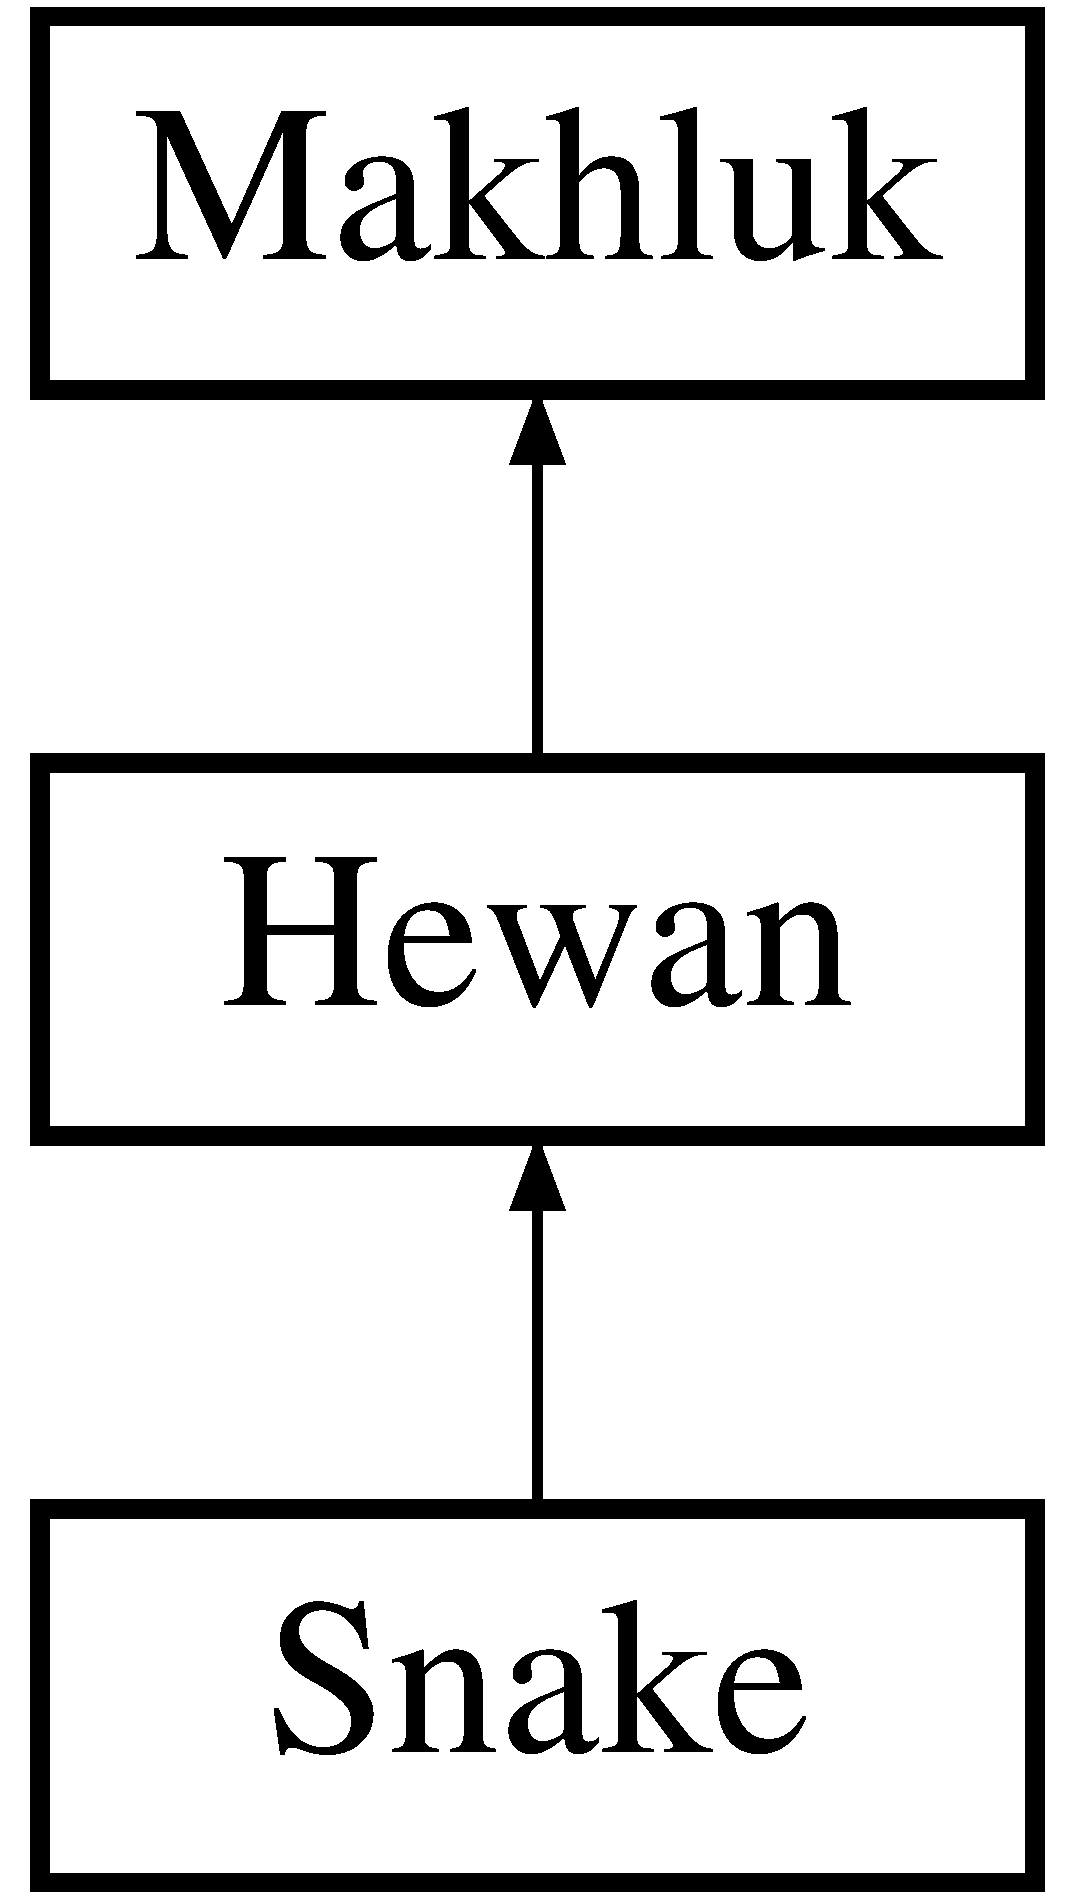
\includegraphics[height=3.000000cm]{class_snake}
\end{center}
\end{figure}
\subsection*{Public Member Functions}
\begin{DoxyCompactItemize}
\item 
{\bfseries Snake} (const \hyperlink{class_point}{Point} \&)\hypertarget{class_snake_a1c1bfb186b5b74d5b8b2bee282e7273e}{}\label{class_snake_a1c1bfb186b5b74d5b8b2bee282e7273e}

\item 
int {\bfseries get\+DeltaT} ()\hypertarget{class_snake_a16c276bca5b03aed618976aeb79d0bdb}{}\label{class_snake_a16c276bca5b03aed618976aeb79d0bdb}

\item 
int \hyperlink{class_snake_a511252859c8eb005b8e4cff200973465}{is\+Vegetarian} ()
\begin{DoxyCompactList}\small\item\em Fungsi pure virtual untuk validasi apakah sebuah objek adalah Vegetarian. \end{DoxyCompactList}\item 
void \hyperlink{class_snake_a605e8e7245842e44f2882395e28b02fe}{Get\+To\+Food} ()
\begin{DoxyCompactList}\small\item\em Procedure virtual pure untuk objek mendapatkan makanannya. \end{DoxyCompactList}\item 
void {\bfseries Zig\+Zag} ()\hypertarget{class_snake_a3921ed0d6fc728f3e1f920d7d2a67184}{}\label{class_snake_a3921ed0d6fc728f3e1f920d7d2a67184}

\item 
void {\bfseries Live} ()\hypertarget{class_snake_a2c340a6cb7f298c2ea7dd1be2c7805fc}{}\label{class_snake_a2c340a6cb7f298c2ea7dd1be2c7805fc}

\end{DoxyCompactItemize}
\subsection*{Additional Inherited Members}


\subsection{Member Function Documentation}
\index{Snake@{Snake}!Get\+To\+Food@{Get\+To\+Food}}
\index{Get\+To\+Food@{Get\+To\+Food}!Snake@{Snake}}
\subsubsection[{\texorpdfstring{Get\+To\+Food()}{GetToFood()}}]{\setlength{\rightskip}{0pt plus 5cm}void Snake\+::\+Get\+To\+Food (
\begin{DoxyParamCaption}
{}
\end{DoxyParamCaption}
)\hspace{0.3cm}{\ttfamily [virtual]}}\hypertarget{class_snake_a605e8e7245842e44f2882395e28b02fe}{}\label{class_snake_a605e8e7245842e44f2882395e28b02fe}


Procedure virtual pure untuk objek mendapatkan makanannya. 

Fungsi pure virtual Get\+To\+Food dideklarasikan pada setiap turunan kelas \hyperlink{class_hewan}{Hewan} untuk mendapatkan makanannya yang berbeda-\/beda \begin{DoxyReturn}{Returns}
void 
\end{DoxyReturn}


Implements \hyperlink{class_hewan_ab0478d48070dc3c51cda481f678ae40a}{Hewan}.

\index{Snake@{Snake}!is\+Vegetarian@{is\+Vegetarian}}
\index{is\+Vegetarian@{is\+Vegetarian}!Snake@{Snake}}
\subsubsection[{\texorpdfstring{is\+Vegetarian()}{isVegetarian()}}]{\setlength{\rightskip}{0pt plus 5cm}int Snake\+::is\+Vegetarian (
\begin{DoxyParamCaption}
{}
\end{DoxyParamCaption}
)\hspace{0.3cm}{\ttfamily [inline]}, {\ttfamily [virtual]}}\hypertarget{class_snake_a511252859c8eb005b8e4cff200973465}{}\label{class_snake_a511252859c8eb005b8e4cff200973465}


Fungsi pure virtual untuk validasi apakah sebuah objek adalah Vegetarian. 

Fungsi pure virtual is\+Vegetarian dideklarasikan pada setiap turunan kelas \hyperlink{class_hewan}{Hewan} \begin{DoxyReturn}{Returns}
int 
\end{DoxyReturn}


Implements \hyperlink{class_hewan_a90a316426af1d53add7ebf2a23ea9af2}{Hewan}.



The documentation for this class was generated from the following files\+:\begin{DoxyCompactItemize}
\item 
C\+:/\+Users/\+Ngiong/\+Documents/\+Git\+Hub/\+Tubes\+Makhluk/header/Snake.\+h\item 
C\+:/\+Users/\+Ngiong/\+Documents/\+Git\+Hub/\+Tubes\+Makhluk/implementation/Snake.\+cpp\end{DoxyCompactItemize}

\hypertarget{class_snapshot_capturer}{}\section{Snapshot\+Capturer Class Reference}
\label{class_snapshot_capturer}\index{Snapshot\+Capturer@{Snapshot\+Capturer}}


Kelas untuk mengambil snapshot state dunia.  




{\ttfamily \#include $<$Snapshot\+Capturer.\+h$>$}

Inheritance diagram for Snapshot\+Capturer\+:\begin{figure}[H]
\begin{center}
\leavevmode
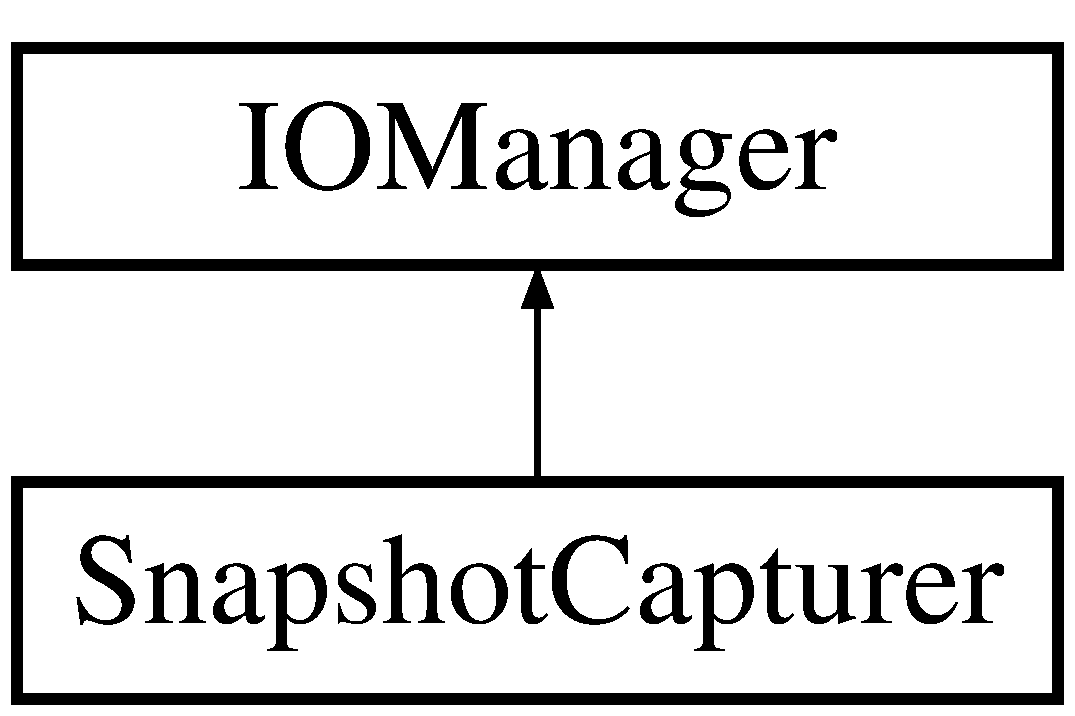
\includegraphics[height=2.000000cm]{class_snapshot_capturer}
\end{center}
\end{figure}
\subsection*{Public Member Functions}
\begin{DoxyCompactItemize}
\item 
void \hyperlink{class_snapshot_capturer_a905be74885968e52e8df43f138260ede}{save\+Old\+Buf} ()
\begin{DoxyCompactList}\small\item\em Menyimpan buffer cout. \end{DoxyCompactList}\item 
void \hyperlink{class_snapshot_capturer_aae816fa4d192adc4eae98fc0fda46db1}{reset\+Cout\+Buf} ()
\begin{DoxyCompactList}\small\item\em Reset buffer cout ke standard output. \end{DoxyCompactList}\item 
void \hyperlink{class_snapshot_capturer_a17c1677e94e0cb1e5a17febbb146c4bc}{capture\+Snapshot} ()
\begin{DoxyCompactList}\small\item\em Mengambil sebuah snapshot state dunia. \end{DoxyCompactList}\end{DoxyCompactItemize}
\subsection*{Static Public Member Functions}
\begin{DoxyCompactItemize}
\item 
static \hyperlink{class_snapshot_capturer}{Snapshot\+Capturer} $\ast$ \hyperlink{class_snapshot_capturer_a7c0367a7b01b5fdebefaa0d83520ffbd}{get\+Capturer\+Instance} ()
\begin{DoxyCompactList}\small\item\em Get Singleton Instance dari kelas \hyperlink{class_snapshot_capturer}{Snapshot\+Capturer}. \end{DoxyCompactList}\end{DoxyCompactItemize}


\subsection{Detailed Description}
Kelas untuk mengambil snapshot state dunia. 

Kelas \hyperlink{class_snapshot_capturer}{Snapshot\+Capturer} bertanggung jawab dalam pengambilan snapshot state dunia dan menyimpan hasil pengambilan snapshot ke sebuah file \begin{DoxyAuthor}{Author}
Robert Sebastian Herlim 
\end{DoxyAuthor}
\begin{DoxyDate}{Date}
Maret 2016 
\end{DoxyDate}


\subsection{Member Function Documentation}
\index{Snapshot\+Capturer@{Snapshot\+Capturer}!capture\+Snapshot@{capture\+Snapshot}}
\index{capture\+Snapshot@{capture\+Snapshot}!Snapshot\+Capturer@{Snapshot\+Capturer}}
\subsubsection[{\texorpdfstring{capture\+Snapshot()}{captureSnapshot()}}]{\setlength{\rightskip}{0pt plus 5cm}void Snapshot\+Capturer\+::capture\+Snapshot (
\begin{DoxyParamCaption}
{}
\end{DoxyParamCaption}
)}\hypertarget{class_snapshot_capturer_a17c1677e94e0cb1e5a17febbb146c4bc}{}\label{class_snapshot_capturer_a17c1677e94e0cb1e5a17febbb146c4bc}


Mengambil sebuah snapshot state dunia. 

Mengambil snapshot state dunia pada saat tertentu dan menuliskan hasil snapshot ke directory file yang tersimpan dalam instance \hyperlink{class_snapshot_capturer}{Snapshot\+Capturer} \begin{DoxyReturn}{Returns}
void 
\end{DoxyReturn}
\index{Snapshot\+Capturer@{Snapshot\+Capturer}!get\+Capturer\+Instance@{get\+Capturer\+Instance}}
\index{get\+Capturer\+Instance@{get\+Capturer\+Instance}!Snapshot\+Capturer@{Snapshot\+Capturer}}
\subsubsection[{\texorpdfstring{get\+Capturer\+Instance()}{getCapturerInstance()}}]{\setlength{\rightskip}{0pt plus 5cm}static {\bf Snapshot\+Capturer}$\ast$ Snapshot\+Capturer\+::get\+Capturer\+Instance (
\begin{DoxyParamCaption}
{}
\end{DoxyParamCaption}
)\hspace{0.3cm}{\ttfamily [inline]}, {\ttfamily [static]}}\hypertarget{class_snapshot_capturer_a7c0367a7b01b5fdebefaa0d83520ffbd}{}\label{class_snapshot_capturer_a7c0367a7b01b5fdebefaa0d83520ffbd}


Get Singleton Instance dari kelas \hyperlink{class_snapshot_capturer}{Snapshot\+Capturer}. 

Mengembalikan pointer dari objek singleton pada kelas \hyperlink{class_snapshot_capturer}{Snapshot\+Capturer} \begin{DoxyReturn}{Returns}
pointer yang menunjuk ke singleton instance pada kelas \hyperlink{class_snapshot_capturer}{Snapshot\+Capturer} 
\end{DoxyReturn}
\index{Snapshot\+Capturer@{Snapshot\+Capturer}!reset\+Cout\+Buf@{reset\+Cout\+Buf}}
\index{reset\+Cout\+Buf@{reset\+Cout\+Buf}!Snapshot\+Capturer@{Snapshot\+Capturer}}
\subsubsection[{\texorpdfstring{reset\+Cout\+Buf()}{resetCoutBuf()}}]{\setlength{\rightskip}{0pt plus 5cm}void Snapshot\+Capturer\+::reset\+Cout\+Buf (
\begin{DoxyParamCaption}
{}
\end{DoxyParamCaption}
)\hspace{0.3cm}{\ttfamily [inline]}}\hypertarget{class_snapshot_capturer_aae816fa4d192adc4eae98fc0fda46db1}{}\label{class_snapshot_capturer_aae816fa4d192adc4eae98fc0fda46db1}


Reset buffer cout ke standard output. 

Mengembalikan buffer cout ke standard output \begin{DoxyReturn}{Returns}
void 
\end{DoxyReturn}
\index{Snapshot\+Capturer@{Snapshot\+Capturer}!save\+Old\+Buf@{save\+Old\+Buf}}
\index{save\+Old\+Buf@{save\+Old\+Buf}!Snapshot\+Capturer@{Snapshot\+Capturer}}
\subsubsection[{\texorpdfstring{save\+Old\+Buf()}{saveOldBuf()}}]{\setlength{\rightskip}{0pt plus 5cm}void Snapshot\+Capturer\+::save\+Old\+Buf (
\begin{DoxyParamCaption}
{}
\end{DoxyParamCaption}
)\hspace{0.3cm}{\ttfamily [inline]}}\hypertarget{class_snapshot_capturer_a905be74885968e52e8df43f138260ede}{}\label{class_snapshot_capturer_a905be74885968e52e8df43f138260ede}


Menyimpan buffer cout. 

Menyimpan buffer cout sekarang ke dalam coutbuf yang tersimpan dalam instance \hyperlink{class_snapshot_capturer}{Snapshot\+Capturer} \begin{DoxyReturn}{Returns}
void 
\end{DoxyReturn}


The documentation for this class was generated from the following files\+:\begin{DoxyCompactItemize}
\item 
C\+:/\+Users/\+Ngiong/\+Documents/\+Git\+Hub/\+Tubes\+Makhluk/v3/header/Snapshot\+Capturer.\+h\item 
C\+:/\+Users/\+Ngiong/\+Documents/\+Git\+Hub/\+Tubes\+Makhluk/v3/implementation/Snapshot\+Capturer.\+cpp\end{DoxyCompactItemize}

\hypertarget{class_tumbuhan}{}\section{Tumbuhan Class Reference}
\label{class_tumbuhan}\index{Tumbuhan@{Tumbuhan}}


Kelas Turunan dari \hyperlink{class_makhluk}{Makhluk} berupa \hyperlink{class_tumbuhan}{Tumbuhan}.  




{\ttfamily \#include $<$Tumbuhan.\+h$>$}

Inheritance diagram for Tumbuhan\+:\begin{figure}[H]
\begin{center}
\leavevmode
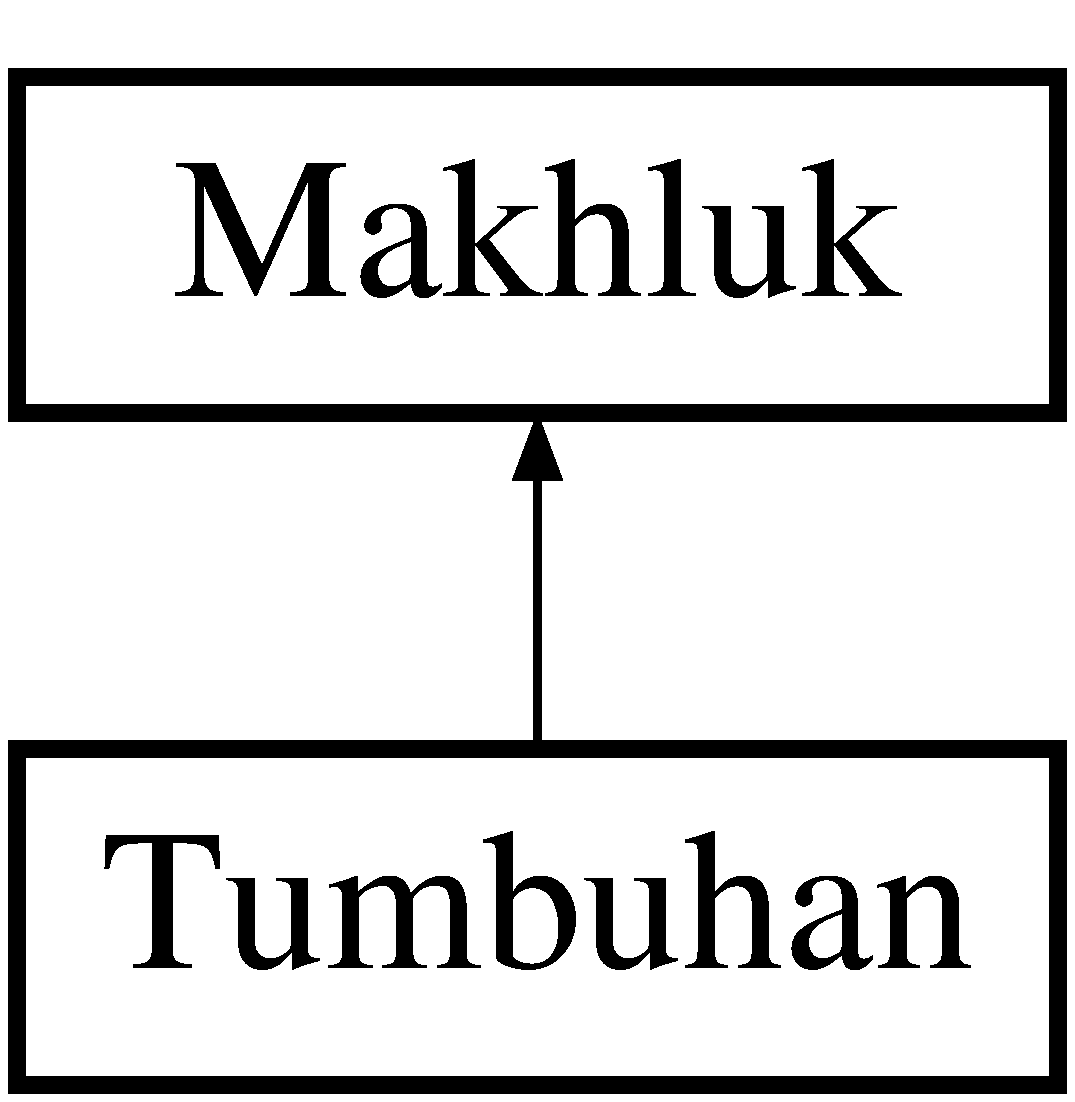
\includegraphics[height=2.000000cm]{class_tumbuhan}
\end{center}
\end{figure}
\subsection*{Public Member Functions}
\begin{DoxyCompactItemize}
\item 
\hyperlink{class_tumbuhan_a3095d94b67888eff7573c5e22620e550}{Tumbuhan} (const \hyperlink{class_point}{Point} \&P)
\begin{DoxyCompactList}\small\item\em Constructor dari objek bertipe \hyperlink{class_tumbuhan}{Tumbuhan}. \end{DoxyCompactList}\item 
void \hyperlink{class_tumbuhan_a18c42e3e111ea943eba9b4dee00ee96b}{Live} ()
\begin{DoxyCompactList}\small\item\em Procedure aksi utama yang mengatur hidup \hyperlink{class_tumbuhan}{Tumbuhan} sampai mati. \end{DoxyCompactList}\item 
void {\bfseries Age\+Increment} ()\hypertarget{class_tumbuhan_a99a110ee2eb38b98e9268565ba796373}{}\label{class_tumbuhan_a99a110ee2eb38b98e9268565ba796373}

\end{DoxyCompactItemize}
\subsection*{Additional Inherited Members}


\subsection{Detailed Description}
Kelas Turunan dari \hyperlink{class_makhluk}{Makhluk} berupa \hyperlink{class_tumbuhan}{Tumbuhan}. 

Kelas \hyperlink{class_tumbuhan}{Tumbuhan} merupakan kelas yang berfungsi untuk mengatur behaviour dan kehidupan dari objek \hyperlink{class_tumbuhan}{Tumbuhan} \begin{DoxyAuthor}{Author}
Elvina Riama K. Situmorang 
\end{DoxyAuthor}
\begin{DoxyDate}{Date}
Maret 2016 
\end{DoxyDate}


\subsection{Constructor \& Destructor Documentation}
\index{Tumbuhan@{Tumbuhan}!Tumbuhan@{Tumbuhan}}
\index{Tumbuhan@{Tumbuhan}!Tumbuhan@{Tumbuhan}}
\subsubsection[{\texorpdfstring{Tumbuhan(const Point \&\+P)}{Tumbuhan(const Point &P)}}]{\setlength{\rightskip}{0pt plus 5cm}Tumbuhan\+::\+Tumbuhan (
\begin{DoxyParamCaption}
\item[{const {\bf Point} \&}]{P}
\end{DoxyParamCaption}
)}\hypertarget{class_tumbuhan_a3095d94b67888eff7573c5e22620e550}{}\label{class_tumbuhan_a3095d94b67888eff7573c5e22620e550}


Constructor dari objek bertipe \hyperlink{class_tumbuhan}{Tumbuhan}. 

Constructor \hyperlink{class_tumbuhan}{Tumbuhan} yang akan membentuk objek bertipe \hyperlink{class_tumbuhan}{Tumbuhan} dengan masukan variable reference \hyperlink{class_point}{Point} sebagai posisi awal objek 
\begin{DoxyParams}{Parameters}
{\em P} & \hyperlink{class_point}{Point} posisi objek akan terbentuk \\
\hline
\end{DoxyParams}
\begin{DoxyReturn}{Returns}
Objek bertipe \hyperlink{class_tumbuhan}{Tumbuhan} 
\end{DoxyReturn}


\subsection{Member Function Documentation}
\index{Tumbuhan@{Tumbuhan}!Live@{Live}}
\index{Live@{Live}!Tumbuhan@{Tumbuhan}}
\subsubsection[{\texorpdfstring{Live()}{Live()}}]{\setlength{\rightskip}{0pt plus 5cm}void Tumbuhan\+::\+Live (
\begin{DoxyParamCaption}
{}
\end{DoxyParamCaption}
)\hspace{0.3cm}{\ttfamily [virtual]}}\hypertarget{class_tumbuhan_a18c42e3e111ea943eba9b4dee00ee96b}{}\label{class_tumbuhan_a18c42e3e111ea943eba9b4dee00ee96b}


Procedure aksi utama yang mengatur hidup \hyperlink{class_tumbuhan}{Tumbuhan} sampai mati. 

Procedure aksi utama akan memilih aktivitas kehidupan yang akan dilakukan oleh \hyperlink{class_tumbuhan}{Tumbuhan} selama hidupnya \begin{DoxyReturn}{Returns}
void 
\end{DoxyReturn}


Implements \hyperlink{class_makhluk}{Makhluk}.



The documentation for this class was generated from the following files\+:\begin{DoxyCompactItemize}
\item 
C\+:/\+Users/\+Ngiong/\+Documents/\+Git\+Hub/\+Tubes\+Makhluk/header/Tumbuhan.\+h\item 
C\+:/\+Users/\+Ngiong/\+Documents/\+Git\+Hub/\+Tubes\+Makhluk/implementation/Tumbuhan.\+cpp\end{DoxyCompactItemize}

\hypertarget{class_turtle}{}\section{Turtle Class Reference}
\label{class_turtle}\index{Turtle@{Turtle}}


Kelas Turunan dari \hyperlink{class_makhluk}{Makhluk} berupa \hyperlink{class_rabbit}{Rabbit}.  




{\ttfamily \#include $<$Turtle.\+h$>$}

Inheritance diagram for Turtle\+:\begin{figure}[H]
\begin{center}
\leavevmode
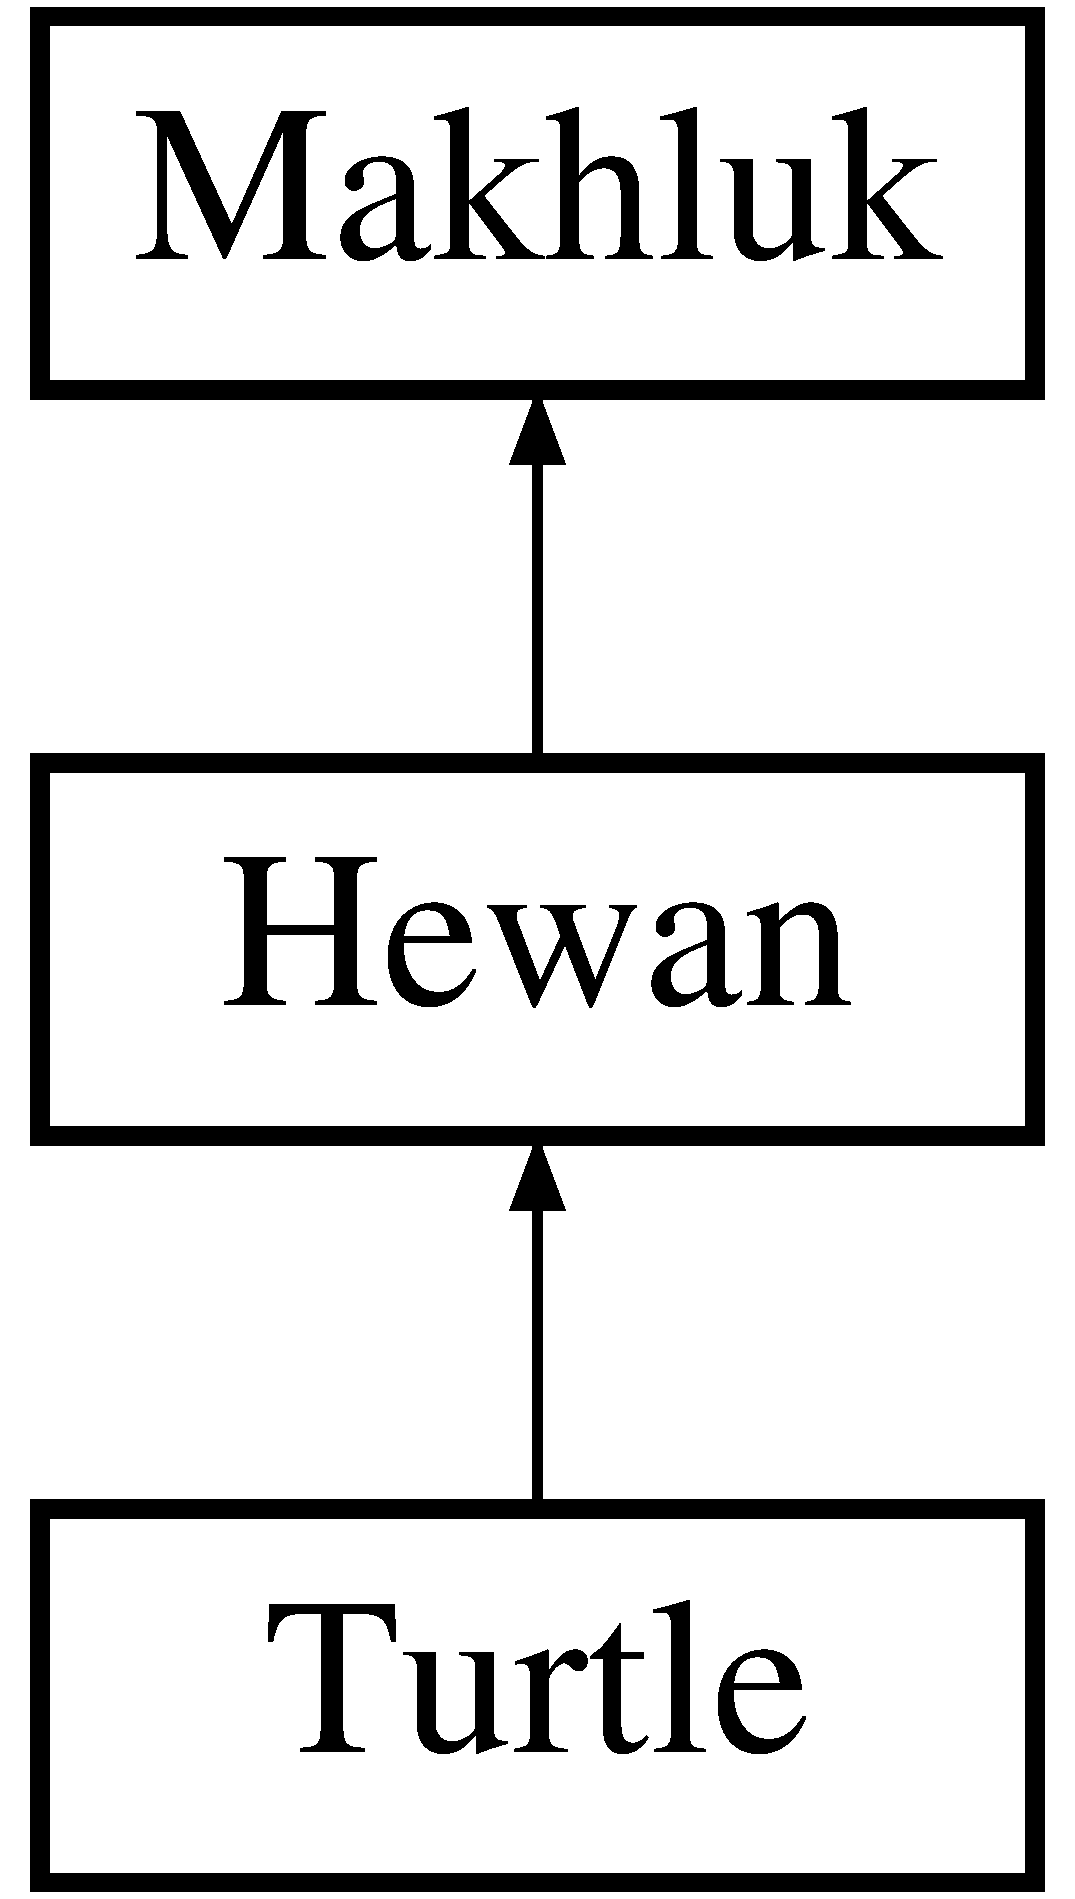
\includegraphics[height=3.000000cm]{class_turtle}
\end{center}
\end{figure}
\subsection*{Public Member Functions}
\begin{DoxyCompactItemize}
\item 
\hyperlink{class_turtle_a1347c5bcaee6ede82a488394cad3cf00}{Turtle} (const \hyperlink{class_point}{Point} \&)
\begin{DoxyCompactList}\small\item\em Constructor dari objek bertipe Turle. \end{DoxyCompactList}\item 
int \hyperlink{class_turtle_aaa6ea76ca2e8b21b18ac65ef4b4663d9}{is\+Vegetarian} ()
\begin{DoxyCompactList}\small\item\em Validasi apakah \hyperlink{class_turtle}{Turtle} merupakan Vegetarian. \end{DoxyCompactList}\item 
int \hyperlink{class_turtle_abeb5244ae5dc51006d3e1d0ca7c048c1}{getis\+Challange} ()
\begin{DoxyCompactList}\small\item\em Getter is\+Challange milik \hyperlink{class_turtle}{Turtle}. \end{DoxyCompactList}\item 
void {\bfseries set\+Is\+Challange} (int a)\hypertarget{class_turtle_a01eb5b88af5f7cc0550ee836be552a37}{}\label{class_turtle_a01eb5b88af5f7cc0550ee836be552a37}

\item 
int \hyperlink{class_turtle_a707d466a9d8ce18d27367b49403249d7}{get\+DeltaT} ()
\begin{DoxyCompactList}\small\item\em Getter DeltaT \hyperlink{class_turtle}{Turtle}. \end{DoxyCompactList}\item 
void \hyperlink{class_turtle_acf11aca3cdcf6aeebac4aac8c2ec416f}{Race} ()
\begin{DoxyCompactList}\small\item\em Procedure aksi untuk \hyperlink{class_turtle}{Turtle} melakukan Race dengan objek \hyperlink{class_rabbit}{Rabbit}. \end{DoxyCompactList}\item 
void \hyperlink{class_turtle_a1f2ab308068556b2621d5acd8eda5413}{Get\+To\+Food} ()
\begin{DoxyCompactList}\small\item\em Procedure aksi untuk \hyperlink{class_rabbit}{Rabbit} mendapatkan makanan. \end{DoxyCompactList}\item 
void \hyperlink{class_turtle_abac9610f1eb0b0894b91cd86173bc257}{Live} ()
\begin{DoxyCompactList}\small\item\em Procedure aksi utama yang mengatur hidup \hyperlink{class_turtle}{Turtle} sampai mati. \end{DoxyCompactList}\end{DoxyCompactItemize}
\subsection*{Static Public Member Functions}
\begin{DoxyCompactItemize}
\item 
static int \hyperlink{class_turtle_ab78b7107247a700a39a443ca4891c1fb}{is\+Any\+Turtle\+Racing} ()
\begin{DoxyCompactList}\small\item\em Validasi apakah ada objek \hyperlink{class_turtle}{Turtle} yang sedang melakukan Race bertipe static function. \end{DoxyCompactList}\end{DoxyCompactItemize}
\subsection*{Additional Inherited Members}


\subsection{Detailed Description}
Kelas Turunan dari \hyperlink{class_makhluk}{Makhluk} berupa \hyperlink{class_rabbit}{Rabbit}. 

Kelas \hyperlink{class_rabbit}{Rabbit} merupakan kelas yang berfungsi untuk mengatur behaviour dan kehidupan dari objek \hyperlink{class_rabbit}{Rabbit} \begin{DoxyAuthor}{Author}
Atika Azzahra Akbar 
\end{DoxyAuthor}
\begin{DoxyDate}{Date}
Maret 2016 
\end{DoxyDate}


\subsection{Constructor \& Destructor Documentation}
\index{Turtle@{Turtle}!Turtle@{Turtle}}
\index{Turtle@{Turtle}!Turtle@{Turtle}}
\subsubsection[{\texorpdfstring{Turtle(const Point \&)}{Turtle(const Point &)}}]{\setlength{\rightskip}{0pt plus 5cm}Turtle\+::\+Turtle (
\begin{DoxyParamCaption}
\item[{const {\bf Point} \&}]{P}
\end{DoxyParamCaption}
)}\hypertarget{class_turtle_a1347c5bcaee6ede82a488394cad3cf00}{}\label{class_turtle_a1347c5bcaee6ede82a488394cad3cf00}


Constructor dari objek bertipe Turle. 

Constructor \hyperlink{class_turtle}{Turtle} yang akan membentuk objek bertipe \hyperlink{class_turtle}{Turtle} dengan masukan variable reference \hyperlink{class_point}{Point} sebagai posisi awal objek \begin{DoxyReturn}{Returns}
Objek bertipe \hyperlink{class_turtle}{Turtle} 
\end{DoxyReturn}


\subsection{Member Function Documentation}
\index{Turtle@{Turtle}!get\+DeltaT@{get\+DeltaT}}
\index{get\+DeltaT@{get\+DeltaT}!Turtle@{Turtle}}
\subsubsection[{\texorpdfstring{get\+Delta\+T()}{getDeltaT()}}]{\setlength{\rightskip}{0pt plus 5cm}int Turtle\+::get\+DeltaT (
\begin{DoxyParamCaption}
{}
\end{DoxyParamCaption}
)\hspace{0.3cm}{\ttfamily [inline]}}\hypertarget{class_turtle_a707d466a9d8ce18d27367b49403249d7}{}\label{class_turtle_a707d466a9d8ce18d27367b49403249d7}


Getter DeltaT \hyperlink{class_turtle}{Turtle}. 

Fungsi getter yang akan mengambilkan nilai deltaT dari \hyperlink{class_turtle}{Turtle} yang merupakan member dari kelas hewan yang diinisialisasi saat ctor \begin{DoxyReturn}{Returns}
Integer DeltaT \hyperlink{class_turtle}{Turtle} 
\end{DoxyReturn}
\index{Turtle@{Turtle}!getis\+Challange@{getis\+Challange}}
\index{getis\+Challange@{getis\+Challange}!Turtle@{Turtle}}
\subsubsection[{\texorpdfstring{getis\+Challange()}{getisChallange()}}]{\setlength{\rightskip}{0pt plus 5cm}int Turtle\+::getis\+Challange (
\begin{DoxyParamCaption}
{}
\end{DoxyParamCaption}
)\hspace{0.3cm}{\ttfamily [inline]}}\hypertarget{class_turtle_abeb5244ae5dc51006d3e1d0ca7c048c1}{}\label{class_turtle_abeb5244ae5dc51006d3e1d0ca7c048c1}


Getter is\+Challange milik \hyperlink{class_turtle}{Turtle}. 

Fungsi getter yang akan mengambilkan nilai is\+Challange dari \hyperlink{class_turtle}{Turtle}. Bernilai 0 jika tidak ada yang mengajak untuk race dan bernilai 1 jika ada \hyperlink{class_rabbit}{Rabbit} yang mengajak \begin{DoxyReturn}{Returns}
Integer 
\end{DoxyReturn}
\index{Turtle@{Turtle}!Get\+To\+Food@{Get\+To\+Food}}
\index{Get\+To\+Food@{Get\+To\+Food}!Turtle@{Turtle}}
\subsubsection[{\texorpdfstring{Get\+To\+Food()}{GetToFood()}}]{\setlength{\rightskip}{0pt plus 5cm}void Turtle\+::\+Get\+To\+Food (
\begin{DoxyParamCaption}
{}
\end{DoxyParamCaption}
)\hspace{0.3cm}{\ttfamily [virtual]}}\hypertarget{class_turtle_a1f2ab308068556b2621d5acd8eda5413}{}\label{class_turtle_a1f2ab308068556b2621d5acd8eda5413}


Procedure aksi untuk \hyperlink{class_rabbit}{Rabbit} mendapatkan makanan. 

Procedure aksi Get\+To\+Food membuat \hyperlink{class_rabbit}{Rabbit} pergi ke point dimana makanannya berasa dan memakannya \begin{DoxyReturn}{Returns}
void 
\end{DoxyReturn}


Implements \hyperlink{class_hewan_ab0478d48070dc3c51cda481f678ae40a}{Hewan}.

\index{Turtle@{Turtle}!is\+Any\+Turtle\+Racing@{is\+Any\+Turtle\+Racing}}
\index{is\+Any\+Turtle\+Racing@{is\+Any\+Turtle\+Racing}!Turtle@{Turtle}}
\subsubsection[{\texorpdfstring{is\+Any\+Turtle\+Racing()}{isAnyTurtleRacing()}}]{\setlength{\rightskip}{0pt plus 5cm}int Turtle\+::is\+Any\+Turtle\+Racing (
\begin{DoxyParamCaption}
{}
\end{DoxyParamCaption}
)\hspace{0.3cm}{\ttfamily [static]}}\hypertarget{class_turtle_ab78b7107247a700a39a443ca4891c1fb}{}\label{class_turtle_ab78b7107247a700a39a443ca4891c1fb}


Validasi apakah ada objek \hyperlink{class_turtle}{Turtle} yang sedang melakukan Race bertipe static function. 

Validasi akan melakukan pencarian \hyperlink{class_makhluk}{Makhluk} \hyperlink{class_turtle}{Turtle} pada list\+Makhluk yang nilai is\+Challange adalah 1 \begin{DoxyReturn}{Returns}
integer 
\end{DoxyReturn}
\index{Turtle@{Turtle}!is\+Vegetarian@{is\+Vegetarian}}
\index{is\+Vegetarian@{is\+Vegetarian}!Turtle@{Turtle}}
\subsubsection[{\texorpdfstring{is\+Vegetarian()}{isVegetarian()}}]{\setlength{\rightskip}{0pt plus 5cm}int Turtle\+::is\+Vegetarian (
\begin{DoxyParamCaption}
{}
\end{DoxyParamCaption}
)\hspace{0.3cm}{\ttfamily [inline]}, {\ttfamily [virtual]}}\hypertarget{class_turtle_aaa6ea76ca2e8b21b18ac65ef4b4663d9}{}\label{class_turtle_aaa6ea76ca2e8b21b18ac65ef4b4663d9}


Validasi apakah \hyperlink{class_turtle}{Turtle} merupakan Vegetarian. 

Validasi akan selalu mengembalikan integer bernilai 1 sebagai validasi bahwa \hyperlink{class_turtle}{Turtle} merupakan binatang vegetarian \begin{DoxyReturn}{Returns}
integer bernilai 1 
\end{DoxyReturn}


Implements \hyperlink{class_hewan_a90a316426af1d53add7ebf2a23ea9af2}{Hewan}.

\index{Turtle@{Turtle}!Live@{Live}}
\index{Live@{Live}!Turtle@{Turtle}}
\subsubsection[{\texorpdfstring{Live()}{Live()}}]{\setlength{\rightskip}{0pt plus 5cm}void Turtle\+::\+Live (
\begin{DoxyParamCaption}
{}
\end{DoxyParamCaption}
)\hspace{0.3cm}{\ttfamily [virtual]}}\hypertarget{class_turtle_abac9610f1eb0b0894b91cd86173bc257}{}\label{class_turtle_abac9610f1eb0b0894b91cd86173bc257}


Procedure aksi utama yang mengatur hidup \hyperlink{class_turtle}{Turtle} sampai mati. 

Procedure aksi utama akan memilih aktivitas kehidupan yang akan dilakukan oleh \hyperlink{class_turtle}{Turtle} selama hidupnya \begin{DoxyReturn}{Returns}
void 
\end{DoxyReturn}


Implements \hyperlink{class_makhluk}{Makhluk}.

\index{Turtle@{Turtle}!Race@{Race}}
\index{Race@{Race}!Turtle@{Turtle}}
\subsubsection[{\texorpdfstring{Race()}{Race()}}]{\setlength{\rightskip}{0pt plus 5cm}void Turtle\+::\+Race (
\begin{DoxyParamCaption}
{}
\end{DoxyParamCaption}
)}\hypertarget{class_turtle_acf11aca3cdcf6aeebac4aac8c2ec416f}{}\label{class_turtle_acf11aca3cdcf6aeebac4aac8c2ec416f}


Procedure aksi untuk \hyperlink{class_turtle}{Turtle} melakukan Race dengan objek \hyperlink{class_rabbit}{Rabbit}. 

Procedure aksi Race ini akan melakukan validasi apakah ada objek \hyperlink{class_rabbit}{Rabbit} yang mengajak race. Jika ada maka \hyperlink{class_turtle}{Turtle} pergi ke point start, dan melakukan race bersama \hyperlink{class_rabbit}{Rabbit} ke finish point \begin{DoxyReturn}{Returns}
void 
\end{DoxyReturn}


The documentation for this class was generated from the following files\+:\begin{DoxyCompactItemize}
\item 
C\+:/\+Users/\+Ngiong/\+Documents/\+Git\+Hub/\+Tubes\+Makhluk/header/Turtle.\+h\item 
C\+:/\+Users/\+Ngiong/\+Documents/\+Git\+Hub/\+Tubes\+Makhluk/implementation/Turtle.\+cpp\end{DoxyCompactItemize}

\hypertarget{class_wolf}{}\section{Wolf Class Reference}
\label{class_wolf}\index{Wolf@{Wolf}}


Kelas turunan dari makhluk berupa \hyperlink{class_wolf}{Wolf}.  




{\ttfamily \#include $<$Wolf.\+h$>$}

Inheritance diagram for Wolf\+:\begin{figure}[H]
\begin{center}
\leavevmode
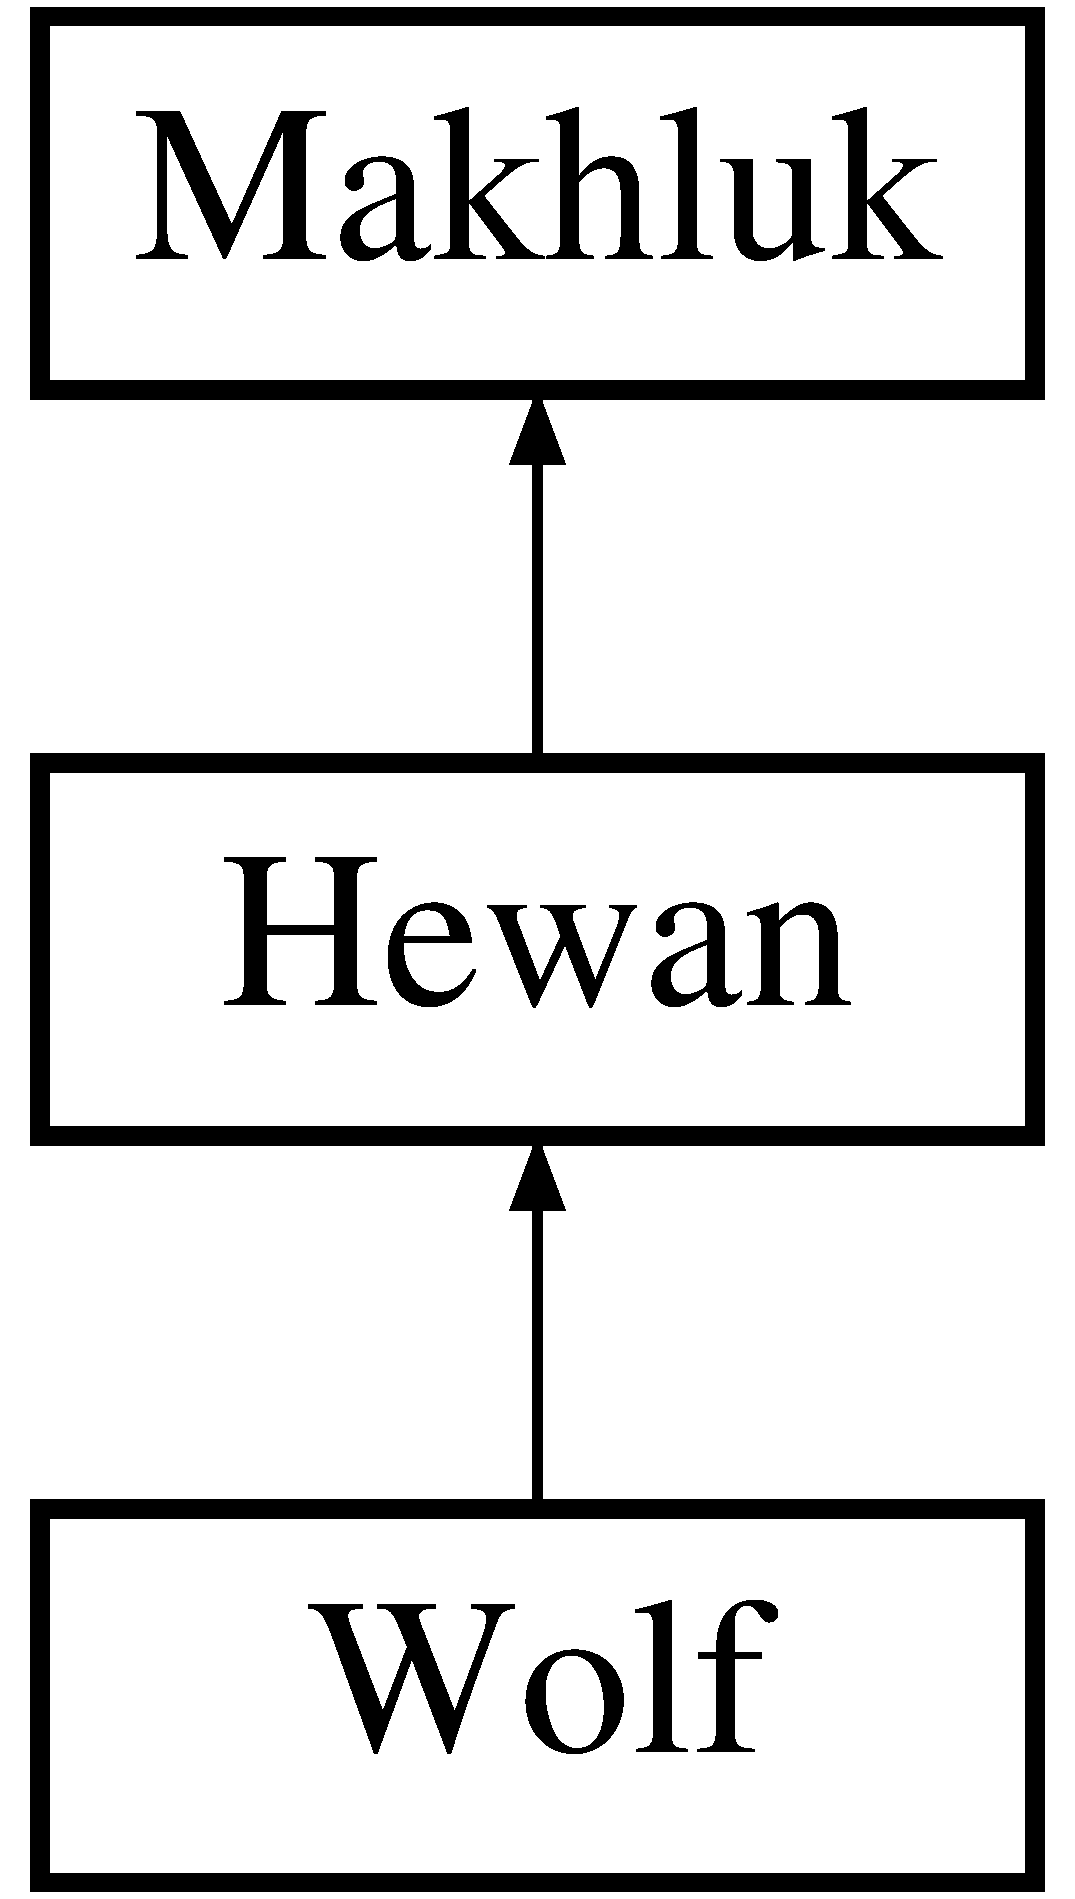
\includegraphics[height=3.000000cm]{class_wolf}
\end{center}
\end{figure}
\subsection*{Public Member Functions}
\begin{DoxyCompactItemize}
\item 
\hyperlink{class_wolf_adb38a4364ecc382ae56e26a2e3f9d7c2}{Wolf} (const \hyperlink{class_point}{Point} \&)
\begin{DoxyCompactList}\small\item\em Constructor. \end{DoxyCompactList}\item 
int \hyperlink{class_wolf_a59589099b9226c3b85fa9c5fb8e51836}{is\+Vegetarian} ()
\begin{DoxyCompactList}\small\item\em Fungsi untuk menentukan apakah \hyperlink{class_wolf}{Wolf} vegetarian. \end{DoxyCompactList}\item 
int \hyperlink{class_wolf_aaab51ccea5bdd26c25ad61e7cb8991a6}{get\+DeltaT} ()
\begin{DoxyCompactList}\small\item\em Getter DeltaT \hyperlink{class_wolf}{Wolf}. \end{DoxyCompactList}\item 
void \hyperlink{class_wolf_a832902ad559bbf8a73bbe16d3378ba86}{Get\+To\+Food} ()
\begin{DoxyCompactList}\small\item\em Prosedur aksi \hyperlink{class_wolf}{Wolf} untuk mendapatkan makanan. \end{DoxyCompactList}\item 
void \hyperlink{class_wolf_a5902349f953664a4d53cc3ddea4b19f3}{Live} ()
\begin{DoxyCompactList}\small\item\em Prosedur hidup \hyperlink{class_wolf}{Wolf}. \end{DoxyCompactList}\end{DoxyCompactItemize}
\subsection*{Additional Inherited Members}


\subsection{Detailed Description}
Kelas turunan dari makhluk berupa \hyperlink{class_wolf}{Wolf}. 

Kelas \hyperlink{class_wolf}{Wolf} merupakan kelas yang berfungsi untuk mengatur behaviour dan kehidupan dari objek \hyperlink{class_wolf}{Wolf} \begin{DoxyAuthor}{Author}
Micky Yudi Utama 
\end{DoxyAuthor}
\begin{DoxyDate}{Date}
Maret 2016 
\end{DoxyDate}


\subsection{Constructor \& Destructor Documentation}
\index{Wolf@{Wolf}!Wolf@{Wolf}}
\index{Wolf@{Wolf}!Wolf@{Wolf}}
\subsubsection[{\texorpdfstring{Wolf(const Point \&)}{Wolf(const Point &)}}]{\setlength{\rightskip}{0pt plus 5cm}Wolf\+::\+Wolf (
\begin{DoxyParamCaption}
\item[{const {\bf Point} \&}]{P}
\end{DoxyParamCaption}
)}\hypertarget{class_wolf_adb38a4364ecc382ae56e26a2e3f9d7c2}{}\label{class_wolf_adb38a4364ecc382ae56e26a2e3f9d7c2}


Constructor. 

Menciptakan objek \hyperlink{class_wolf}{Wolf} dengan posisi P 
\begin{DoxyParams}{Parameters}
{\em P} & const \hyperlink{class_point}{Point}\& Posisi objek \hyperlink{class_wolf}{Wolf} \\
\hline
\end{DoxyParams}


\subsection{Member Function Documentation}
\index{Wolf@{Wolf}!get\+DeltaT@{get\+DeltaT}}
\index{get\+DeltaT@{get\+DeltaT}!Wolf@{Wolf}}
\subsubsection[{\texorpdfstring{get\+Delta\+T()}{getDeltaT()}}]{\setlength{\rightskip}{0pt plus 5cm}int Wolf\+::get\+DeltaT (
\begin{DoxyParamCaption}
{}
\end{DoxyParamCaption}
)\hspace{0.3cm}{\ttfamily [inline]}}\hypertarget{class_wolf_aaab51ccea5bdd26c25ad61e7cb8991a6}{}\label{class_wolf_aaab51ccea5bdd26c25ad61e7cb8991a6}


Getter DeltaT \hyperlink{class_wolf}{Wolf}. 

Fungsi untuk memperoleh DeltaT makhluk \hyperlink{class_wolf}{Wolf} \begin{DoxyReturn}{Returns}
Bilangan bulat berupa DeltaT \hyperlink{class_wolf}{Wolf} 
\end{DoxyReturn}
\index{Wolf@{Wolf}!Get\+To\+Food@{Get\+To\+Food}}
\index{Get\+To\+Food@{Get\+To\+Food}!Wolf@{Wolf}}
\subsubsection[{\texorpdfstring{Get\+To\+Food()}{GetToFood()}}]{\setlength{\rightskip}{0pt plus 5cm}void Wolf\+::\+Get\+To\+Food (
\begin{DoxyParamCaption}
{}
\end{DoxyParamCaption}
)\hspace{0.3cm}{\ttfamily [virtual]}}\hypertarget{class_wolf_a832902ad559bbf8a73bbe16d3378ba86}{}\label{class_wolf_a832902ad559bbf8a73bbe16d3378ba86}


Prosedur aksi \hyperlink{class_wolf}{Wolf} untuk mendapatkan makanan. 

Prosedur aksi \hyperlink{class_wolf}{Wolf} untuk pergi ke makanannya \begin{DoxyReturn}{Returns}
void 
\end{DoxyReturn}


Implements \hyperlink{class_hewan_ab0478d48070dc3c51cda481f678ae40a}{Hewan}.

\index{Wolf@{Wolf}!is\+Vegetarian@{is\+Vegetarian}}
\index{is\+Vegetarian@{is\+Vegetarian}!Wolf@{Wolf}}
\subsubsection[{\texorpdfstring{is\+Vegetarian()}{isVegetarian()}}]{\setlength{\rightskip}{0pt plus 5cm}int Wolf\+::is\+Vegetarian (
\begin{DoxyParamCaption}
{}
\end{DoxyParamCaption}
)\hspace{0.3cm}{\ttfamily [inline]}, {\ttfamily [virtual]}}\hypertarget{class_wolf_a59589099b9226c3b85fa9c5fb8e51836}{}\label{class_wolf_a59589099b9226c3b85fa9c5fb8e51836}


Fungsi untuk menentukan apakah \hyperlink{class_wolf}{Wolf} vegetarian. 

Fungsi akan selalu mengembalikan bilangan bulat 0 karena \hyperlink{class_wolf}{Wolf} bukan vegetarian \begin{DoxyReturn}{Returns}
Bilangan bulat 0 
\end{DoxyReturn}


Implements \hyperlink{class_hewan_a90a316426af1d53add7ebf2a23ea9af2}{Hewan}.

\index{Wolf@{Wolf}!Live@{Live}}
\index{Live@{Live}!Wolf@{Wolf}}
\subsubsection[{\texorpdfstring{Live()}{Live()}}]{\setlength{\rightskip}{0pt plus 5cm}void Wolf\+::\+Live (
\begin{DoxyParamCaption}
{}
\end{DoxyParamCaption}
)\hspace{0.3cm}{\ttfamily [virtual]}}\hypertarget{class_wolf_a5902349f953664a4d53cc3ddea4b19f3}{}\label{class_wolf_a5902349f953664a4d53cc3ddea4b19f3}


Prosedur hidup \hyperlink{class_wolf}{Wolf}. 

Prosedur untuk menentukan apa yang akan dilakukan oleh \hyperlink{class_wolf}{Wolf} ketika masih hidup \begin{DoxyReturn}{Returns}
void 
\end{DoxyReturn}


Implements \hyperlink{class_makhluk}{Makhluk}.



The documentation for this class was generated from the following files\+:\begin{DoxyCompactItemize}
\item 
C\+:/\+Users/\+Ngiong/\+Documents/\+Git\+Hub/\+Tubes\+Makhluk/header/Wolf.\+h\item 
C\+:/\+Users/\+Ngiong/\+Documents/\+Git\+Hub/\+Tubes\+Makhluk/implementation/Wolf.\+cpp\end{DoxyCompactItemize}

\hypertarget{class_world}{}\section{World Class Reference}
\label{class_world}\index{World@{World}}


Representasi dari alam semesta.  




{\ttfamily \#include $<$World.\+h$>$}

\subsection*{Public Member Functions}
\begin{DoxyCompactItemize}
\item 
\hyperlink{class_l_makhluk}{L\+Makhluk} $\ast$ \hyperlink{class_world_af9625fa1995e0c3bbdb3e6e7d48effa2}{get\+Objects} ()
\begin{DoxyCompactList}\small\item\em Get List of \hyperlink{class_makhluk}{Makhluk}. \end{DoxyCompactList}\item 
int \hyperlink{class_world_ab77dab54a1e3e7b5657b39f05cb0d2a5}{get\+N\+Brs} ()
\begin{DoxyCompactList}\small\item\em Get jumlah baris. \end{DoxyCompactList}\item 
int \hyperlink{class_world_a2d8ed3b33860324182e773fde59832b2}{get\+N\+Kol} ()
\begin{DoxyCompactList}\small\item\em Get jumlah kolom. \end{DoxyCompactList}\item 
void \hyperlink{class_world_ab166a5835416154c7276dcfa8c523e2e}{Print\+Map} ()
\begin{DoxyCompactList}\small\item\em Print dunia beserta isinya. \end{DoxyCompactList}\item 
int \hyperlink{class_world_acd627d79b89688184df6e9601ffe1532}{is\+Ended} ()
\begin{DoxyCompactList}\small\item\em Get status is\+Ended. \end{DoxyCompactList}\item 
int \hyperlink{class_world_ad06b05aabbcbe0c93106793bdb5fcc2c}{is\+Paused} ()
\begin{DoxyCompactList}\small\item\em Get status is\+Paused. \end{DoxyCompactList}\item 
void \hyperlink{class_world_a30a87c6071aef420fc2e9df913a7452d}{end\+World} ()
\begin{DoxyCompactList}\small\item\em Mengakhiri aktivitas dunia. \end{DoxyCompactList}\item 
void \hyperlink{class_world_a1df17b17270667dc2ff9ff52f6ade6c0}{change\+Pause\+State} ()
\begin{DoxyCompactList}\small\item\em Mengubah status berjalannya aktivitas dunia. \end{DoxyCompactList}\item 
void \hyperlink{class_world_a63197059e4c4f18349aec3c1daa66a01}{lock\+World} ()
\begin{DoxyCompactList}\small\item\em Memberhentikan aktivitas dunia. \end{DoxyCompactList}\item 
void \hyperlink{class_world_a08481fdff65e290c44386676ce993dce}{unlock\+World} ()
\begin{DoxyCompactList}\small\item\em Melanjutkan aktivitas dunia. \end{DoxyCompactList}\end{DoxyCompactItemize}
\subsection*{Static Public Member Functions}
\begin{DoxyCompactItemize}
\item 
static \hyperlink{class_world}{World} $\ast$ \hyperlink{class_world_a7a8d0b3f76f0ecde36ffe28f9b08f30f}{get\+World\+Instance} ()
\begin{DoxyCompactList}\small\item\em Get Singleton Instance dari kelas \hyperlink{class_world}{World}. \end{DoxyCompactList}\item 
static void \hyperlink{class_world_a5013e1294abc50b60ffa747bcd4499f4}{Show} (int)
\begin{DoxyCompactList}\small\item\em Print dunia beserta isinya secara berkala. \end{DoxyCompactList}\end{DoxyCompactItemize}


\subsection{Detailed Description}
Representasi dari alam semesta. 

Kelas \hyperlink{class_world}{World} merepresentasikan alam semesta yang terdiri dari sebuah \char`\"{}ruang\char`\"{} (space) fiktif yang memiliki dimensi panjang dan lebar dan sekumpulan makhluk-\/makhluk (objects) yang bisa bergerak secara independen. \begin{DoxyAuthor}{Author}
Robert Sebastian Herlim 
\end{DoxyAuthor}
\begin{DoxyDate}{Date}
Maret 2016 
\end{DoxyDate}


\subsection{Member Function Documentation}
\index{World@{World}!change\+Pause\+State@{change\+Pause\+State}}
\index{change\+Pause\+State@{change\+Pause\+State}!World@{World}}
\subsubsection[{\texorpdfstring{change\+Pause\+State()}{changePauseState()}}]{\setlength{\rightskip}{0pt plus 5cm}void World\+::change\+Pause\+State (
\begin{DoxyParamCaption}
{}
\end{DoxyParamCaption}
)}\hypertarget{class_world_a1df17b17270667dc2ff9ff52f6ade6c0}{}\label{class_world_a1df17b17270667dc2ff9ff52f6ade6c0}


Mengubah status berjalannya aktivitas dunia. 

Mengubah status is\+Paused menjadi kebalikannya, yang mengakibatkan apabila dunia sedang bergerak akan berhenti dan apabila dunia sedang berhenti akan bergerak kembali \begin{DoxyReturn}{Returns}
void 
\end{DoxyReturn}
\index{World@{World}!end\+World@{end\+World}}
\index{end\+World@{end\+World}!World@{World}}
\subsubsection[{\texorpdfstring{end\+World()}{endWorld()}}]{\setlength{\rightskip}{0pt plus 5cm}void World\+::end\+World (
\begin{DoxyParamCaption}
{}
\end{DoxyParamCaption}
)\hspace{0.3cm}{\ttfamily [inline]}}\hypertarget{class_world_a30a87c6071aef420fc2e9df913a7452d}{}\label{class_world_a30a87c6071aef420fc2e9df913a7452d}


Mengakhiri aktivitas dunia. 

Mengubah status is\+Ended menjadi T\+R\+UE yang menandakan dunia sudah berakhir \begin{DoxyReturn}{Returns}
void 
\end{DoxyReturn}
\index{World@{World}!get\+N\+Brs@{get\+N\+Brs}}
\index{get\+N\+Brs@{get\+N\+Brs}!World@{World}}
\subsubsection[{\texorpdfstring{get\+N\+Brs()}{getNBrs()}}]{\setlength{\rightskip}{0pt plus 5cm}int World\+::get\+N\+Brs (
\begin{DoxyParamCaption}
{}
\end{DoxyParamCaption}
)\hspace{0.3cm}{\ttfamily [inline]}}\hypertarget{class_world_ab77dab54a1e3e7b5657b39f05cb0d2a5}{}\label{class_world_ab77dab54a1e3e7b5657b39f05cb0d2a5}


Get jumlah baris. 

Mengembalikan jumlah baris yang merupakan dimensi panjang dari ukuran ruang dunia \begin{DoxyReturn}{Returns}
Bilangan bulat yang menyatakan dimensi panjang dari ukuran ruang dunia 
\end{DoxyReturn}
\index{World@{World}!get\+N\+Kol@{get\+N\+Kol}}
\index{get\+N\+Kol@{get\+N\+Kol}!World@{World}}
\subsubsection[{\texorpdfstring{get\+N\+Kol()}{getNKol()}}]{\setlength{\rightskip}{0pt plus 5cm}int World\+::get\+N\+Kol (
\begin{DoxyParamCaption}
{}
\end{DoxyParamCaption}
)\hspace{0.3cm}{\ttfamily [inline]}}\hypertarget{class_world_a2d8ed3b33860324182e773fde59832b2}{}\label{class_world_a2d8ed3b33860324182e773fde59832b2}


Get jumlah kolom. 

Mengembalikan jumlah kolom yang merupakan dimensi lebar dari ukuran ruang dunia \begin{DoxyReturn}{Returns}
Bilangan bulat yang menyatakan dimensi lebar dari ukuran ruang dunia 
\end{DoxyReturn}
\index{World@{World}!get\+Objects@{get\+Objects}}
\index{get\+Objects@{get\+Objects}!World@{World}}
\subsubsection[{\texorpdfstring{get\+Objects()}{getObjects()}}]{\setlength{\rightskip}{0pt plus 5cm}{\bf L\+Makhluk}$\ast$ World\+::get\+Objects (
\begin{DoxyParamCaption}
{}
\end{DoxyParamCaption}
)\hspace{0.3cm}{\ttfamily [inline]}}\hypertarget{class_world_af9625fa1995e0c3bbdb3e6e7d48effa2}{}\label{class_world_af9625fa1995e0c3bbdb3e6e7d48effa2}


Get List of \hyperlink{class_makhluk}{Makhluk}. 

Mengambil list of makhluk-\/makhluk yang hidup di dalam dunia tersebut \begin{DoxyReturn}{Returns}
List yang berisi pointer ke makhluk-\/makhluk yang ada dalam dunia 
\end{DoxyReturn}
\index{World@{World}!get\+World\+Instance@{get\+World\+Instance}}
\index{get\+World\+Instance@{get\+World\+Instance}!World@{World}}
\subsubsection[{\texorpdfstring{get\+World\+Instance()}{getWorldInstance()}}]{\setlength{\rightskip}{0pt plus 5cm}static {\bf World}$\ast$ World\+::get\+World\+Instance (
\begin{DoxyParamCaption}
{}
\end{DoxyParamCaption}
)\hspace{0.3cm}{\ttfamily [inline]}, {\ttfamily [static]}}\hypertarget{class_world_a7a8d0b3f76f0ecde36ffe28f9b08f30f}{}\label{class_world_a7a8d0b3f76f0ecde36ffe28f9b08f30f}


Get Singleton Instance dari kelas \hyperlink{class_world}{World}. 

Mengembalikan pointer dari objek singleton pada kelas \hyperlink{class_world}{World} \begin{DoxyReturn}{Returns}
pointer yang menunjuk ke singleton instance pada kelas \hyperlink{class_world}{World} 
\end{DoxyReturn}
\index{World@{World}!is\+Ended@{is\+Ended}}
\index{is\+Ended@{is\+Ended}!World@{World}}
\subsubsection[{\texorpdfstring{is\+Ended()}{isEnded()}}]{\setlength{\rightskip}{0pt plus 5cm}int World\+::is\+Ended (
\begin{DoxyParamCaption}
{}
\end{DoxyParamCaption}
)\hspace{0.3cm}{\ttfamily [inline]}}\hypertarget{class_world_acd627d79b89688184df6e9601ffe1532}{}\label{class_world_acd627d79b89688184df6e9601ffe1532}


Get status is\+Ended. 

Predikat untuk menyatakan apakah aktivitas dunia sudah berakhir \begin{DoxyReturn}{Returns}
T\+R\+UE apabila aktivitas dunia sudah berakhir 
\end{DoxyReturn}
\index{World@{World}!is\+Paused@{is\+Paused}}
\index{is\+Paused@{is\+Paused}!World@{World}}
\subsubsection[{\texorpdfstring{is\+Paused()}{isPaused()}}]{\setlength{\rightskip}{0pt plus 5cm}int World\+::is\+Paused (
\begin{DoxyParamCaption}
{}
\end{DoxyParamCaption}
)\hspace{0.3cm}{\ttfamily [inline]}}\hypertarget{class_world_ad06b05aabbcbe0c93106793bdb5fcc2c}{}\label{class_world_ad06b05aabbcbe0c93106793bdb5fcc2c}


Get status is\+Paused. 

Predikat untuk menyatakan apakah aktivitas dunia sedang diberhentikan \begin{DoxyReturn}{Returns}
T\+R\+UE apabila aktivitas dunia sudah berakhir 
\end{DoxyReturn}
\index{World@{World}!lock\+World@{lock\+World}}
\index{lock\+World@{lock\+World}!World@{World}}
\subsubsection[{\texorpdfstring{lock\+World()}{lockWorld()}}]{\setlength{\rightskip}{0pt plus 5cm}void World\+::lock\+World (
\begin{DoxyParamCaption}
{}
\end{DoxyParamCaption}
)}\hypertarget{class_world_a63197059e4c4f18349aec3c1daa66a01}{}\label{class_world_a63197059e4c4f18349aec3c1daa66a01}


Memberhentikan aktivitas dunia. 

Mengubah status is\+Paused menjadi T\+R\+UE, dan memberhentikan semua aktivitas dunia \begin{DoxyReturn}{Returns}
void 
\end{DoxyReturn}
\index{World@{World}!Print\+Map@{Print\+Map}}
\index{Print\+Map@{Print\+Map}!World@{World}}
\subsubsection[{\texorpdfstring{Print\+Map()}{PrintMap()}}]{\setlength{\rightskip}{0pt plus 5cm}void World\+::\+Print\+Map (
\begin{DoxyParamCaption}
{}
\end{DoxyParamCaption}
)}\hypertarget{class_world_ab166a5835416154c7276dcfa8c523e2e}{}\label{class_world_ab166a5835416154c7276dcfa8c523e2e}


Print dunia beserta isinya. 

Mencetak state dunia beserta dengan makhluk-\/makhluk yang ada di dalamnya ke layar \begin{DoxyReturn}{Returns}
void 
\end{DoxyReturn}
\index{World@{World}!Show@{Show}}
\index{Show@{Show}!World@{World}}
\subsubsection[{\texorpdfstring{Show(int)}{Show(int)}}]{\setlength{\rightskip}{0pt plus 5cm}void World\+::\+Show (
\begin{DoxyParamCaption}
\item[{int}]{deltaT}
\end{DoxyParamCaption}
)\hspace{0.3cm}{\ttfamily [static]}}\hypertarget{class_world_a5013e1294abc50b60ffa747bcd4499f4}{}\label{class_world_a5013e1294abc50b60ffa747bcd4499f4}


Print dunia beserta isinya secara berkala. 

Mencetak state dunia beserta dengan isi-\/isinya ke layar secara berkala dengan interval waktu tertentu 
\begin{DoxyParams}{Parameters}
{\em deltaT} & int interval waktu (dalam ms) antar pencetakan state dunia ke layar \\
\hline
\end{DoxyParams}
\begin{DoxyReturn}{Returns}
void 
\end{DoxyReturn}
\index{World@{World}!unlock\+World@{unlock\+World}}
\index{unlock\+World@{unlock\+World}!World@{World}}
\subsubsection[{\texorpdfstring{unlock\+World()}{unlockWorld()}}]{\setlength{\rightskip}{0pt plus 5cm}void World\+::unlock\+World (
\begin{DoxyParamCaption}
{}
\end{DoxyParamCaption}
)}\hypertarget{class_world_a08481fdff65e290c44386676ce993dce}{}\label{class_world_a08481fdff65e290c44386676ce993dce}


Melanjutkan aktivitas dunia. 

Mengubah status is\+Paused menjadi F\+A\+L\+SE, dan menjalankan kembali semua aktivitas dunia \begin{DoxyReturn}{Returns}
void 
\end{DoxyReturn}


The documentation for this class was generated from the following files\+:\begin{DoxyCompactItemize}
\item 
C\+:/\+Users/\+Ngiong/\+Documents/\+Git\+Hub/\+Tubes\+Makhluk/header/World.\+h\item 
C\+:/\+Users/\+Ngiong/\+Documents/\+Git\+Hub/\+Tubes\+Makhluk/implementation/World.\+cpp\end{DoxyCompactItemize}

\hypertarget{class_world_builder}{}\section{World\+Builder Class Reference}
\label{class_world_builder}\index{World\+Builder@{World\+Builder}}


Builder kelas \hyperlink{class_world}{World}.  




{\ttfamily \#include $<$World\+Builder.\+h$>$}

\subsection*{Public Member Functions}
\begin{DoxyCompactItemize}
\item 
string \hyperlink{class_world_builder_a9fca5be466395c4367aa5d6eb7e2020f}{get\+Str\+Makhluk} ()
\begin{DoxyCompactList}\small\item\em Get string makhluk. \end{DoxyCompactList}\item 
void \hyperlink{class_world_builder_abcb1fda856eebc76d5f5d3a9cf5127f5}{set\+Str\+Makhluk} (const string \&\+\_\+str)
\begin{DoxyCompactList}\small\item\em Setter string makhluk. \end{DoxyCompactList}\item 
void \hyperlink{class_world_builder_ac063d96facdcd9c1c34e69e418d6f733}{build\+World\+Objects} ()
\begin{DoxyCompactList}\small\item\em Build \hyperlink{class_world}{World} Objects. \end{DoxyCompactList}\end{DoxyCompactItemize}
\subsection*{Static Public Member Functions}
\begin{DoxyCompactItemize}
\item 
static \hyperlink{class_world_builder}{World\+Builder} $\ast$ \hyperlink{class_world_builder_ad6b3457a2a185135f33fde9e5939145a}{get\+Builder\+Instance} ()
\begin{DoxyCompactList}\small\item\em Get Singleton Instance dari kelas \hyperlink{class_world_builder}{World\+Builder}. \end{DoxyCompactList}\end{DoxyCompactItemize}


\subsection{Detailed Description}
Builder kelas \hyperlink{class_world}{World}. 

Kelas \hyperlink{class_world_builder}{World\+Builder} merupakan B\+U\+I\+L\+D\+ER dari kelas \hyperlink{class_world}{World}, dan bertanggung jawab untuk melakukan inisialisasi objek-\/objek dunia \begin{DoxyAuthor}{Author}
Robert Sebastian Herlim 
\end{DoxyAuthor}
\begin{DoxyDate}{Date}
Maret 2016 
\end{DoxyDate}


\subsection{Member Function Documentation}
\index{World\+Builder@{World\+Builder}!build\+World\+Objects@{build\+World\+Objects}}
\index{build\+World\+Objects@{build\+World\+Objects}!World\+Builder@{World\+Builder}}
\subsubsection[{\texorpdfstring{build\+World\+Objects()}{buildWorldObjects()}}]{\setlength{\rightskip}{0pt plus 5cm}void World\+Builder\+::build\+World\+Objects (
\begin{DoxyParamCaption}
{}
\end{DoxyParamCaption}
)}\hypertarget{class_world_builder_ac063d96facdcd9c1c34e69e418d6f733}{}\label{class_world_builder_ac063d96facdcd9c1c34e69e418d6f733}


Build \hyperlink{class_world}{World} Objects. 

Melakukan inisialisasi list of makhluk pada objek singleton kelas \hyperlink{class_world}{World} berdasarkan string yang tersimpan dalam instance \hyperlink{class_world_builder}{World\+Builder} \begin{DoxyReturn}{Returns}
void 
\end{DoxyReturn}
\index{World\+Builder@{World\+Builder}!get\+Builder\+Instance@{get\+Builder\+Instance}}
\index{get\+Builder\+Instance@{get\+Builder\+Instance}!World\+Builder@{World\+Builder}}
\subsubsection[{\texorpdfstring{get\+Builder\+Instance()}{getBuilderInstance()}}]{\setlength{\rightskip}{0pt plus 5cm}static {\bf World\+Builder}$\ast$ World\+Builder\+::get\+Builder\+Instance (
\begin{DoxyParamCaption}
{}
\end{DoxyParamCaption}
)\hspace{0.3cm}{\ttfamily [inline]}, {\ttfamily [static]}}\hypertarget{class_world_builder_ad6b3457a2a185135f33fde9e5939145a}{}\label{class_world_builder_ad6b3457a2a185135f33fde9e5939145a}


Get Singleton Instance dari kelas \hyperlink{class_world_builder}{World\+Builder}. 

Mengembalikan pointer dari objek singleton pada kelas \hyperlink{class_world_builder}{World\+Builder} \begin{DoxyReturn}{Returns}
pointer yang menunjuk ke singleton instance pada kelas \hyperlink{class_world_builder}{World\+Builder} 
\end{DoxyReturn}
\index{World\+Builder@{World\+Builder}!get\+Str\+Makhluk@{get\+Str\+Makhluk}}
\index{get\+Str\+Makhluk@{get\+Str\+Makhluk}!World\+Builder@{World\+Builder}}
\subsubsection[{\texorpdfstring{get\+Str\+Makhluk()}{getStrMakhluk()}}]{\setlength{\rightskip}{0pt plus 5cm}string World\+Builder\+::get\+Str\+Makhluk (
\begin{DoxyParamCaption}
{}
\end{DoxyParamCaption}
)\hspace{0.3cm}{\ttfamily [inline]}}\hypertarget{class_world_builder_a9fca5be466395c4367aa5d6eb7e2020f}{}\label{class_world_builder_a9fca5be466395c4367aa5d6eb7e2020f}


Get string makhluk. 

Mengembalikan sebuah string yang tersimpan dalam instance \hyperlink{class_world_builder}{World\+Builder} yang merupakan karakter-\/karakter makhluk yang akan diciptakan \begin{DoxyReturn}{Returns}
string yang berisi karakter-\/karakter makhluk yang akan diciptakan 
\end{DoxyReturn}
\index{World\+Builder@{World\+Builder}!set\+Str\+Makhluk@{set\+Str\+Makhluk}}
\index{set\+Str\+Makhluk@{set\+Str\+Makhluk}!World\+Builder@{World\+Builder}}
\subsubsection[{\texorpdfstring{set\+Str\+Makhluk(const string \&\+\_\+str)}{setStrMakhluk(const string &_str)}}]{\setlength{\rightskip}{0pt plus 5cm}void World\+Builder\+::set\+Str\+Makhluk (
\begin{DoxyParamCaption}
\item[{const string \&}]{\+\_\+str}
\end{DoxyParamCaption}
)\hspace{0.3cm}{\ttfamily [inline]}}\hypertarget{class_world_builder_abcb1fda856eebc76d5f5d3a9cf5127f5}{}\label{class_world_builder_abcb1fda856eebc76d5f5d3a9cf5127f5}


Setter string makhluk. 

Melakukan assignment string yang tersimpan dalam instance \hyperlink{class_world_builder}{World\+Builder} dengan string baru yang di-\/passing melalui parameter 
\begin{DoxyParams}{Parameters}
{\em \+\_\+str} & const string\& String baru yang akan di-\/assign \\
\hline
\end{DoxyParams}
\begin{DoxyReturn}{Returns}
void 
\end{DoxyReturn}


The documentation for this class was generated from the following files\+:\begin{DoxyCompactItemize}
\item 
C\+:/\+Users/\+Ngiong/\+Documents/\+Git\+Hub/\+Tubes\+Makhluk/header/World\+Builder.\+h\item 
C\+:/\+Users/\+Ngiong/\+Documents/\+Git\+Hub/\+Tubes\+Makhluk/implementation/World\+Builder.\+cpp\end{DoxyCompactItemize}

%--- End generated contents ---

% Index
\backmatter
\newpage
\phantomsection
\clearemptydoublepage
\addcontentsline{toc}{chapter}{Index}
\printindex

\end{document}
